\documentclass[a4paper,10pt]{article}
\usepackage{geometry} %Per impostare i  margini del foglio
 \geometry{
 a4paper,
 total={170mm,257mm},
 left=20mm,
 top=20mm,
 }
%\setcounter{secnumdepth}{1} %per subsection non numerate ma nell'indice
\usepackage[italian]{babel} %Mette in italiano tutte le parole fisse di LaTeX (v. "TITOLO")
\usepackage[utf8]{inputenc} %Gestisce i caratteri accentati
\usepackage{comment} %Per  usare \begin{comment}
\usepackage{amsthm} %per gli ambienti theorem
\usepackage{amsmath} %cose matematiche
\usepackage{amssymb} %cose matematiche
\usepackage{mathrsfs} %per \mathscr
\usepackage{dsfont} %per \mathds{1}
\usepackage{mathtools}
\usepackage{float}
\usepackage{units} %per \nicefrac{}{} 
\usepackage{cancel} %per \cancel{}
\usepackage{caption} %mettere le descrizioni
\usepackage{graphicx} %Importare foto
\usepackage{booktabs}
%\pagestyle{empty} %per togliere il numero della pagina
\usepackage{xcolor} %per \color{} e \textcolor{}{}
\usepackage{empheq} 
%\usepackage{enumitem} %Insieme  ai vari \renewcommand per fare elenchi coi numeri belli
\usepackage[shortlabels]{enumitem}
\usepackage{physics} %Per avere \nabla in grassetto
\usepackage[most]{tcolorbox} %Box colorati teoremi
\usepackage{mdframed}
\usepackage{framed}
\usepackage{color,soul} %per evidenziare con il comando highlight \hl
\usepackage{hyperref} %per URL (con \url{}) e hyperlink
\usepackage{tikz} %robe  disegnate
\usepackage{tikz-cd}
\usetikzlibrary{matrix,shapes}
\usepackage{color}
\definecolor{shadecolor}{rgb}{0.902344, 0.902344, 0.902344}
\usepackage{wasysym} %per \lightning


%DA BARABBA%%%%%%%%%%%%%%%%%%%%%%%%%%%%%%%%%%%%%%%%%%%%%%%%%%%%%%%%%%%%%%%%%%%
%\usepackage{tikz}
%\usepackage[unicode=true,pdfusetitle,
% bookmarks=true,bookmarksnumbered=false,bookmarksopen=false,
% breaklinks=false,pdfborder={0 0 1},backref=false,colorlinks=false]
% {hyperref}
\usepackage{changepage}

\usepackage{array}
\usepackage{float}
\usepackage{booktabs}
\usepackage{calc}
\usepackage{units}
\usepackage{mathrsfs}
\usepackage{mathtools}
\usepackage{enumitem}
\usepackage{todonotes}
\usepackage{amsmath}
\usepackage{amsthm}
\usepackage{amssymb}
\usepackage{cancel}
\usepackage{wasysym}
\PassOptionsToPackage{obeyFinal}{todonotes}

\newlist{casenv}{enumerate}{4}
\setlist[casenv]{leftmargin=*,align=left,widest={iiii}}
\setlist[casenv,1]{label={{\itshape\ \casename} \arabic*.},ref=\arabic*}
\setlist[casenv,2]{label={{\itshape\ \casename} \roman*.},ref=\roman*}
\setlist[casenv,3]{label={{\itshape\ \casename\ \alph*.}},ref=\alph*}
\setlist[casenv,4]{label={{\itshape\ \casename} \arabic*.},ref=\arabic*}

\providecommand{\exercisename}{Esercizio}
\theoremstyle{definition}
\newtheorem*{xca*}{\protect\exercisename}

\renewcommand{\labelenumi}{(\roman{enumi})}

\DeclareMathOperator*{\rot}{rot}
%\DeclareMathOperator*{\divergence}{div}
\DeclareMathOperator*{\mis}{mis}
\DeclareMathOperator*{\vers}{vers}
\DeclareMathOperator*{\diag}{diag}

%%%%%%%%%%%%%%%%%%%%%%%%%%%%%% LyX specific LaTeX commands.
\newcommand{\noun}[1]{\textsc{#1}}
\newcommand{\lyxmathsym}[1]{\ifmmode\begingroup\def\b@ld{bold}
  \text{\ifx\math@version\b@ld\bfseries\fi#1}\endgroup\else#1\fi}

%% Because html converters don't know tabularnewline
\providecommand{\tabularnewline}{\\}
%%%%%%%%%%%%%%%%%%%%%%%%%%%%%%%%%%%%%%%%%%%%%%%%%%%%%%%%%%%%%%%%%%%




%%%%%%%%%%%%%%%%%%%%%%%%%%%%%%%%%%%%%%%%%%%%%%%%%%%%%%%%%%%%%%%%%%%%%%%%%%%%%%%%%%%%%%%%%%%%%
%RINOMINA DI COMANDI
%\renewcommand{\labelenumii}{\arabic{enumi}.\arabic{enumii}}
%\renewcommand{\labelenumiii}{\arabic{enumi}.\arabic{enumii}.\arabic{enumiii}}
%\renewcommand{\labelenumiv}{\arabic{enumi}.\arabic{enumii}.\arabic{enumiii}.\arabic{enumiv}}

\newcommand{\bv}{\boldsymbol} %per scrivere i vettori in  grassetto usare \bv
\newcommand{\cv}[2]{\begin{pmatrix} #1 \\ #2 \end{pmatrix}} %column vector di due dim
\newcommand{\cvv}[3]{\begin{pmatrix} #1 \\ #2 \\ #3 \end{pmatrix}} %column vector di tre dim
\newcommand{\myth}{\normalfont \scshape \textcolor{red}} %mio modo custom di mettere teoremi/lemmi/proposizioni
\newcommand{\re}{\mathbb{R}} %numeri reali
\newcommand{\na}{\mathbb{N}} %numeri naturali
\newcommand{\pr}{\text{I\kern-0.15em P}} %probabilità
\newcommand{\ex}{\mathbb{E}} %operatore valore atteso/media
\newcommand{\om}{\Omega} %spazio campionario
\newcommand{\F}{\mathcal{F}} %%sigma algebra, famiglia degli eventi
\newcommand{\myeq}[1]{\stackrel{\mathclap{\normalfont\mbox{\tiny{#1}}}}{=}} %scrivere soppra all'uguale con \myeq{<cosa voglio scrivere>}
\newcommand{\mylist}[1]{\textnormal{\textsc{#1}}}
\newcommand{\notimplies}{%
\mathrel{{\ooalign{\hidewidth$\not\phantom{=}$\hidewidth\cr$\implies$}}}}  %per \notimplies

\newcommand\myfunc[5]{         %per scrivere funzioni con dominio, codominio e dove va un elemento
  \begingroup
  \setlength\arraycolsep{0pt}
  #1\colon\begin{array}[t]{c >{{}}c<{{}} c}
             #2 & \to & #3 \\ #4 & \mapsto & #5 
          \end{array}%
  \endgroup}

%%%%%%%%%%%%%%%%%%%%%%%%%%%%%%%%%%%%%%%%%%%%%%%%%%%%%%%%%%%%%%%%%%%%%%%%%%%%%%%%%%%%%%%%%%%%%
%NUOVI STILI
\newtheoremstyle{indentdefinition}
{5mm}                % Space above
{5mm}                % Space below
{\addtolength{\leftskip}{0mm}\setlength{\parindent}{0em}}        % Theorem body font % (default is "\upshape")
{0mm}                % Indent amount
{\bfseries}       % Theorem head font % (default is \mdseries)
{:}               % Punctuation after theorem head % default: no punctuation
{ }               % Space after theorem head
{\thmname{#1} \thmnumber{#2} \thmnote{\textnormal{(\textcolor{blue}{#3})}}}                % Theorem head spec

\newtheoremstyle{indenttheorem}
{5mm}                % Space above
{5mm}                % Space below
{\addtolength{\leftskip}{10mm}\setlength{\parindent}{0em}}        % Theorem body font % (default is "\upshape")
{-10mm}                % Indent amount
{\bfseries\scshape\color{red}}       % Theorem head font % (default is \mdseries)
{.}               % Punctuation after theorem head % default: no punctuation
{ }               % Space after theorem head
{\thmname{#1} \thmnumber{#2} \thmnote{(\textnormal{#3})}}                % Theorem head spec

\newtheoremstyle{myremark}
{5mm}                % Space above
{5mm}                % Space below
{}        % Theorem body font % (default is "\upshape")
{}                % Indent amount
{\itshape}       % Theorem head font % (default is \mdseries)
{}               % Punctuation after theorem head % default: no punctuation
{ }               % Space after theorem head
{\thmname{#1} \thmnote{(\textbf{#3})}}                % Theorem head spec

\newtheoremstyle{indentgeneral}
{5mm}                % Space above
{5mm}                % Space below
{\addtolength{\leftskip}{10mm}\setlength{\parindent}{0em}}        % Theorem body font % (default is "\upshape")
{-10mm}                % Indent amount
{}       % Theorem head font % (default is \mdseries)
{}               % Punctuation after theorem head % default: no punctuation
{3mm}               % Space after theorem head
{\thmnote{\textbf{#3}}}                % Theorem head spec

%%%%%%%%%%%%%%%%%%%%%%%%%%%%%%%%%%%%%%%%%%%%%%%%%%%%%%%%%%%%%%%%%%%%%%%%%%%%%%%%%%%%%%%%%%%%%
%NUOVI AMBIENTI

\theoremstyle{indentdefinition}
\newtheorem{defn}{Definizione}[section]

\theoremstyle{indenttheorem}
\newtheorem{thm}{Teo.}
\newtheorem{prop}{Prop.}
\newtheorem{lem*}{Lemma}
\newtheorem{cor}{Cor.}

\theoremstyle{myremark}
\newtheorem*{rem*}{Osservazione}
\newtheorem{example*}{Esempio}
\newtheorem{notation*}{Notazione}

\theoremstyle{indentgeneral}
\newtheorem*{gen}{}

\newenvironment{dimo}{\begin{quote}\textit{\textbf{Dimostrazione.}}}{\end{quote}} %dimostrazione con indentatura
\newenvironment{lyxlist}[1]
	{\begin{list}{}
		{\settowidth{\labelwidth}{#1}
		 \setlength{\leftmargin}{\labelwidth}
		 \addtolength{\leftmargin}{\labelsep}
		 \renewcommand{\makelabel}[1]{##1\hfil}}}
	{\end{list}}

\newsavebox{\mybox}  %per ambiente \myboxed
\newenvironment{myboxed} 
{\noindent\begin{lrbox}{\mybox}\begin{minipage}{\textwidth}}
{\end{minipage}\end{lrbox}\fbox{\usebox{\mybox}}}


%\tcolorboxenvironment{theorem}{
%enhanced jigsaw,colframe=black,interior hidden, breakable,before skip=10pt,after skip=10pt }

%\tcolorboxenvironment{prop}{
%enhanced jigsaw,colframe=black,interior hidden, breakable,before skip=10pt,after skip=10pt }

%\tcolorboxenvironment{lem*}{
%enhanced jigsaw,colframe=black,interior hidden, breakable,before skip=10pt,after skip=10pt }

%\tcolorboxenvironment{eq}{
%enhanced jigsaw,colframe=orange,interior hidden, breakable,before skip=10pt,after skip=10pt }

%\tcolorboxenvironment{defin}{
%enhanced jigsaw,colframe=cyan,interior hidden, breakable,before skip=10pt,after skip=10pt }

%\tcolorboxenvironment{prop}{
%enhanced jigsaw,colframe=yellow,interior hidden, breakable,before skip=10pt,after skip=10pt }

\title{\textbf{Meccanica Razionale}}
\author{Alessandro Sosso, Marco Ambrogio Bergamo}
\date{Anno 2023-2024}

\begin{document}
\maketitle
\tableofcontents{}

\section*{Preliminari}
\begin{defn}[Spazio affine reale]
    di dimensione $n$: ${A}^n$ insieme i cui elementi si dicono punti con la seguente struttura:
    \begin{itemize}[leftmargin=15mm]
        \item \textbf{spazio vettoriale delle traslazioni / dei vettori liberi:}   $V$ spazio vettoriale di dim. $n$
        \item \textbf{operazione differenza:} $\phi: A^n\times A^n \to V \mid (p,q)\mapsto (P-Q)$ con le proprietà:
        \begin{itemize}
            \item per ogni coppia $(P,\bv{v})$, $P\in A^n,\bv{v}\in V$ esiste un unico punto $Q\in A \mid P-Q=\bv{v}$
            \item (regola parallelogramma) $(P-Q)+(Q-R)=P-R \quad \forall p,q,R$
        \end{itemize}
    \end{itemize}
\end{defn}

\begin{defn}[Vettore applicato]
la coppia $(P,\bv{v})$ dove  $P\in A^n,\bv{v}\in V$
\end{defn}

\begin{defn}[Spazio euclideo]
    $(A^n, \cdot)$ dove $A^n$ spazio affine e $\cdot$ prodotto scalare e distanza $d\left(p,q\right)=\sqrt{\left\Vert \boldsymbol{PQ}\right\Vert }$. 
\end{defn}

\subsection{Operazioni tra vettori}

\begin{gen}[Prodotto vettoriale]
$\times:V\times V \to V$ tale che $|\bv{u}\times \bv{v}|=|\bv{u}||\bv{v}|\sin\theta$, direzione $\perp$ al piano dei vettori, verso (mano destra).\\
Gode delle proprietà:
\begin{itemize}[leftmargin=15mm]
    \item lineare nell'argomento di sinistra
    \item antisimmetrico
    \item non associativo
\end{itemize}
Fissato un sit. di rif. $\Sigma=\{O,\bv{e}_1,\bv{e}_2,\bv{e}_3\}$ allora $$\bv{u}\times \bv{v} = \begin{vmatrix} \bv{e}_1 & \bv{e}_2 & \bv{e}_3 \\ u_1 & u_2 & u_3 \\ v_1 & v_2 & v_3\end{vmatrix}$$
\end{gen}

\begin{gen}[Prodotto misto]
lo scalare $(\bv{u}\times \bv{v})\cdot\bv{w}$ \\
Prorpietà:
\begin{itemize}[leftmargin=15mm]
\item invariante per permutazione circolare dei fattori
\item coincide (a meno di segno) con volume del parallelepipedo costruito sui tre vettori
\end{itemize}
\end{gen}

\begin{gen}[Doppio prodotto vettoriale]
$\left(a\times b\right)\times c=\left(a\cdot c\right)b-\left(b\cdot c\right)a$
\end{gen}

\begin{gen}[Equazione vettoriale]
$x\times a=b$. Se $a,b\neq0$ ha
soluzione $\iff$ $b\cdot a=0$. La soluzione generale è dunque
\[
x=\frac{1}{a^{2}}\left(a\times b\right)+\lambda a \qquad\lambda\in\re
\]
\end{gen}
\begin{dimo}
    Doppio prod. vettoriale: $$(a\times b)\times a=(a\cdot a)b - (b\cdot a)a=a^2b-0 \implies b= \frac{1}{a^2}[(a\times b)\times a] $$
    Sostituisco:
    \begin{align*}
    x\times a &= \frac{1}{a^2}[(a\times b)\times a] \\
    x\times a - \frac{1}{a^2}[(a\times b)\times a] &= 0 \\
     (x - \frac{1}{a^2}(a\times b))\times a &= 0 \implies \text{tesi}
     \end{align*}
    
\end{dimo}


\section{Cinematica}
Punto in moto nello spazio euclideo
\subsection{Riferimenti}
\begin{defn}[Riferimento cartesiano]
    nello spazio affine $A^n$ è costituito da un'\textbf{origine} $O\in A^n$ e una \textbf{base} $\{\bv{v}_1\dots \bv{v}_n\}$ dello sp. $V$. Si indica con $\Sigma=\{O, \bv{v}_1\dots \bv{v}_n\}$
    \begin{itemize}[leftmargin=15mm]
        \item \textbf{Punto nel riferimento cartesiano} assegnato un $\Sigma$, ogni punto $P\in A^n$ si identifica con la $n$-upla delle componenti del vettore $P-O$ rispetto alla base $$\bv{r}=P-O=\begin{pmatrix} x_1 \\ \vdots \\ x_n \end{pmatrix}$$
        \item \textbf{Riferimento cartesiano ortogonale}(nel caso $n=3$) $\Sigma=\mathscr{E}\coloneqq\{O,\bv{e}_1,\bv{e}_2,\bv{e}_3\}$, con $\bv{e}_i\cdot \bv{e}_j=\delta_{ij}$
    \end{itemize}
\end{defn}

\begin{defn}[Riferimento non cartesiano - coordinate curvilinee]
    Considerare l'applicazione di cambiamento di coordinate:
    \begin{align*}
    Q\subset \re^n  & \to  D \subseteq \re^n \\
       \bv{q}=\begin{pmatrix} q_1 \\ \vdots \\ q_n \end{pmatrix} & \mapsto  \bv{x}(\bv{q})=  \begin{pmatrix} x_1(q_1\dots q_n) \\ \vdots \\ x_n(q_1\dots q_n) \end{pmatrix}\\
    \end{align*}
    con le proprietà: di classe $C^1(Q)$ e la Jacobiana $J=\begin{pmatrix}
            \pdv{x_1}{q_1} \dots \pdv{x_1}{q_n} \\ \vdots \\ \pdv{x_n}{q_1} \dots \pdv{x_n}{q_n}
        \end{pmatrix}$ di rango massimo \\
        Chiamiamo le coordinate $x_1\dots x_n= \bv{x}(\bv{q})$ coordinate curvilinee.
\end{defn}

\begin{defn}[Base locale]
    sono i vettori $$\bv{u}_1(\bv{x})=\pdv{\bv{x}}{q_1},\dots,\bv{u}_n(\bv{x})=\pdv{\bv{x}}{q_n}$$
    essendo $J$ di rango massimo, i suoi vettori colonnaformano una base dello spazio $V$ 
\end{defn}

\begin{rem*}
    I vettori della base locale sono tangenti alle linee coordinate corrispondenti (tengo fisse $n-1$ coordinate e ne vario una): $\bv{u}_i$ tangente a $\bv{x}(q_i)$
\end{rem*}

\begin{example*}[Coordinate polari]
    Linee coordinate sono circonferenze e assi polari
    \begin{itemize}
        \item Riferimento: $\Sigma=\{O,\boldsymbol{e}_{1},\boldsymbol{e}_{2}\}$. Tutti i vettori colonna saranno intesi in questa base
        \item Coordinate:  $\bv{q}=(\rho,\theta) \quad \bv{x}=\cv{x}{y} \quad  \bv{x}(\bv{q})=\cv{\rho\cos\theta}{\rho\sin\theta}$
        \item Jacobiana: $\begin{pmatrix}
            \cos\theta & -\rho\sin\theta \\ \sin\theta & \rho\cos\theta
        \end{pmatrix}$
        \item Base locale: 
        \begin{align*}
            \bv{u}_1=\frac{\partial\bv{x}}{\partial \rho} & =\cv{\cos\theta}{\sin\theta}, \quad \bv{u}_2 =\frac{\partial\bv{x}}{\partial \theta}= \cv{-\rho\sin\theta}{\rho\cos\theta} \\
            \bv{e}_\rho & =\cv{\cos\theta}{\sin\theta}, \quad \bv{e}_\theta  = \frac{\bv{u}_2}{\rho}=\cv{-\sin\theta}{\cos\theta} 
        \end{align*}
        In particolare si ha $$\begin{cases}
            \bv{u}_1=\bv{e}_\rho \\
            \bv{u}_2=\rho\bv{e}_\theta
        \end{cases}$$
     NB: ho dovuto  dividere $\bv{e}_\theta$ per $\rho$ per tenerlo di modulo 1. Infatti $\bv{e}_\theta$ è il rate of change di $\bv{x}$ al variare in maniera costante di $\theta$, $\pdv{\bv{x}}{\theta}$ che è tanto maggiore quanto è maggiore il raggio. \\
Ricordiamo che $\bv{u}_1$ è tangente a $\bv{x}(\rho)$, ovvero agli assi polari, mentre $\bv{u}_2$ è tangente a $\bv{x}(\theta)$, ovvero alle circonferenze. Quindi $\bv{e}_\rho$ è la componente radiale, mentre $\bv{e}_\theta$ è la componente tangente alle circonferenze.
    \end{itemize}
\end{example*}
\begin{example*}[Coordinate sferiche]
    \nameref{fig:coordinate-sferiche}  Linee coordinate sono i paralleli, i meridiani e gli assi polari.
\begin{figure}[h]
        \centering
        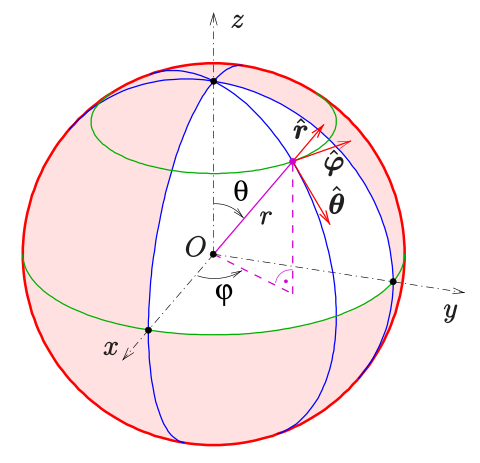
\includegraphics[width=0.25\linewidth]{image.png}
        \caption{Coordinate sferiche}
        \label{fig:coordinate-sferiche}
    \end{figure}
    \begin{itemize}
        \item Riferimento: $\Sigma=\{O,\bv{e}_1,\boldsymbol{e}_{2},\boldsymbol{e}_{3}\}$. Tutti i vettori colonna saranno intesi in questa base
        \item Coordinate:  $\bv{q}=(\rho,\phi,\theta) \quad \bv{x}=\cvv{x}{y}{z} \quad  \bv{x}(\bv{q})=\cvv{\rho\sin\theta\cos\phi}{\rho\sin\theta\sin\phi}{\rho\cos\theta}$ \\
dove $\phi$ è la longitudine (angolo con asse $x$) e $\theta$ la latitudine (angolo con asse $z$). Ricorda $\rho\sin\theta$ proietta il punto sul piano $xy$.
        \item Jacobiana: $\left(\frac{\partial \bv{x}}{\partial q_1},\frac{\partial \bv{x}}{\partial q_2},\frac{\partial \bv{x}}{\partial q_3}\right)=\begin{pmatrix}
            \sin\theta\cos\phi & -\rho\sin\theta\sin\phi & \rho\cos\theta\cos\phi \\
            \sin\theta\sin\phi & \rho\sin\theta\cos\phi & \rho\cos\theta\sin\phi \\
            \cos\theta & 0 & -\rho\sin\phi
        \end{pmatrix}$
        \item Base locale: colonne della Jacobiana e normalizzo. Quindi si ha:
        $$\begin{cases}
            \bv{u}_\rho=\bv{e}_\rho \\
            \bv{u}_\phi=\rho\sin\theta\bv{e}_\phi \\
            \bv{u}_\theta=\rho \bv{e}_\theta
        \end{cases}$$
   \end{itemize}
\end{example*}

\subsection{Cinematica del punto}
$t\in I\subset \re,\quad I\to\mathscr{E}:\; t\mapsto P(t)$
\paragraph{Coordinate cartesiane}

$\Sigma=\left\{ 0,\boldsymbol{e}_{1},\boldsymbol{e}_{2},\boldsymbol{e}_{3}\right\} $
\begin{lyxlist}{00.00.0000}
\item [{{Posizione}}] $\boldsymbol{r}\left(t\right)=P\left(t\right)-O=\cvv{{x}_1(t)}{{x}_2(t)}{{x}_3(t)}$
(sostegno $\gamma\colon\left[t_{0},t\right]\rightarrow\mathbb{R}^3$)
\item [{{Velocità}}] $\boldsymbol{v}\left(t\right)=\frac{d\boldsymbol{r}\left(t\right)}{dt}=\dot{\bv{x}}(t)=\cvv{\dot{x}_1(t)}{\dot{x}_2(t)}{\dot{x}_3(t)}$
\item [{{Accelerazione}}] $\boldsymbol{a}\left(t\right)=\frac{d\boldsymbol{v}\left(t\right)}{dt}=\ddot{x}_{1}\boldsymbol{e}_{1}+\ddot{x}_{2}\boldsymbol{e}_{2}+\ddot{x}_{3}\boldsymbol{e}_{3}$
\end{lyxlist}
Per derivare un vettore si può anche scrivere come combinazione lineare della base e derivare normalmente  (con linearità e derivata del prodotto)

\paragraph{Coordinate curvulinee} 
\begin{description}
    \item[\textnormal{\textsc{Posizione}}] $\bv{x}((\bv{q}(t))$
    \item[\mylist{Velocità (in base locale)}]  $\bv{v}=\frac{d}{dt}(\bv{x}(\bv{q}(t))) = J(\bv{x}(\bv{q}))\cdot\dot{\bv{q}}= \frac{d\bv{x}}{d\bv{q}}\frac{d\bv{q}}{dt}=\pdv{\bv{x}}{q_1}\dot{q_1}+\pdv{\bv{x}}{q_2}\dot{q_2}+\pdv{\bv{x}}{q_3}\dot{q_3}=\dot{q_1}\bv{u}_1+\dot{q_2}\bv{u}_2+\dot{q_3}\bv{u}_3 \rightarrow$ vettore velocità nella base locale
\end{description}

\paragraph{Coordinate polari}

$\Sigma=\left\{ 0,\boldsymbol{e}_{1},\boldsymbol{e}_{2}\right\} $,
$\begin{cases}
x(\rho,\theta)=\rho\cos\theta\\
y(\rho,\theta)=\rho\sin\theta
\end{cases}$, $P=P(t) \implies \rho(t), \theta(t)$
\begin{description}

\item [\mylist{Posizione}] $\boldsymbol{r}\left(t\right)=\rho\cdot\boldsymbol{e}_{\rho}$
con $\boldsymbol{e}_{\rho}=\cv{\cos\theta}{\sin\theta}$
\item [\mylist{Velocità}] $\boldsymbol{v}=\dot{q_1}\bv{u}_1+\dot{q_2}\bv{u}_2=\dot{\rho}\bv{e}_\rho+\dot{\theta}\rho\bv{e}_\theta$ (come da coordinate curvilinee) oppure $\bv{v}(t)=\frac{d}{dt}\rho\bv{e}_\rho=\dot{\rho}\bv{e}_\rho+\rho\dot{\theta}\bv{e}_\theta$
\begin{description}
    \item [\mylist{Radiale}] $\dot{\rho}$
    \item [\mylist{Trasversa}] $\rho\dot{\theta}$
\end{description}
\item [\mylist{Accelerazione}] $\boldsymbol{a}=\frac{d}{dt}\left(\dot{\rho}\boldsymbol{e}_{\rho}+\rho\dot{\theta}\boldsymbol{e}_{\theta}\right)=\underbrace{\left(\ddot{\rho}-\rho\dot{\theta}^{2}\right)}_{\text{Radiale}}\boldsymbol{e}_{\rho}+\underbrace{\left(\rho\ddot{\theta}+2\dot{\rho}\dot{\theta}\right)}_{\text{Trasversa}}\boldsymbol{e}_{\theta}$
\end{description}
\begin{rem*}
    $\begin{cases}
        \frac{d}{dt}\bv{e}_\rho=\frac{d}{dt}(\cos\theta(t)\bv{e}_1+\sin\theta(t)\bv{e}_2 )=\dot{\theta}\bv{e}_\theta \\
        \frac{d}{dt}\bv{e}_\theta=\frac{d}{dt}(-\sin\theta\bv{e}_1+\cos\theta\bv{e}_2)= -\dot{\theta}\bv{e}_\rho
        
    \end{cases} \qquad \frac{d}{d\theta}\bv{e}_\rho= \bv{e_\theta}$
\end{rem*}

\paragraph{Coordinate sferiche} 
\begin{description}
    \item[\mylist{Posizione}] $\bv{r}(t)=\rho\bv{e}_\rho$
    \item[\mylist{Velocità}] $\bv{v}=\dot{q_1}\bv{u}_1+\dot{q_2}\bv{u}_2+\dot{q_3}\bv{u}_3=\dot{\rho}\bv{e}_\rho+\underbrace{\dot{\phi}\rho\sin\theta}_{\text{Longitudinale}}\bv{e}_\phi+\underbrace{\rho\dot{\theta}}_{\text{Latitudinale}}\bv{e}_\theta $ 
\end{description}
\paragraph{Coordinate cilindriche}

$\Sigma=\left\{ 0,\boldsymbol{e}_{1},\boldsymbol{e}_{2},\boldsymbol{e}_{3}\right\} $,
$\begin{cases}
x=\rho\cos\theta\\
y=\rho\sin\theta\\
z=z
\end{cases}$
\begin{description}
\item [\mylist{Posizione}] $\boldsymbol{r}\left(t\right)=\rho\cdot\boldsymbol{u}_{\rho}+z\boldsymbol{u}_{z}$
con $\boldsymbol{u}_{\rho}=\boldsymbol{e}_{1}\cos\theta+\boldsymbol{e}_{2}\sin\theta$
\item [\mylist{Velocità}] $\boldsymbol{v}=\dot{\rho}\boldsymbol{u}_{\rho}+\rho\dot{\theta}\boldsymbol{u}_{\theta}+\dot{z}\boldsymbol{u}_{z}$
\item [\mylist{Accelerazione}] $\boldsymbol{a}=\left(\ddot{\rho}-\rho\dot{\theta}^{2}\right)\boldsymbol{u}_{\rho}+\left(\rho\ddot{\theta}+2\dot{\rho}\dot{\theta}\right)\boldsymbol{u}_{\theta}+\ddot{z}\boldsymbol{u}_{z}$
\end{description}

\subsection{Curve parametrizzate}
\begin{defn}[lunghezza di una curva]
\label{def:lunghezza-curva}$l=\int_{a}^{b}\sqrt{\bv{\alpha}'\left(t\right)\cdot\boldsymbol{\alpha}'\left(t\right)}dt=\int_{a}^{b}\left|\boldsymbol{\alpha}'\left(t\right)\right|dt$,
con $\boldsymbol{\alpha}$ curva parametrizzata regolare.
\end{defn}

\begin{defn}[parametro naturale]
\label{def:parametro-naturale}$s\left(t\right)=\pm\int_{0}^{t}\left|\dot{\boldsymbol{r}}\left(\tau\right)\right|d\tau$,
e dunque $\left|\frac{d\boldsymbol{r}}{ds}\left(s\right)\right|=1\;\forall s$.
\end{defn}
\begin{rem*}
    $|\bv{s}'(t)|=|\bv{x}'(t)|$
\end{rem*}
\begin{defn}[triedro di Frenet]
\label{def:triedro-Frenet}$\left(\boldsymbol{t},\boldsymbol{n},\boldsymbol{b}\right)$
con
\begin{align*}
\boldsymbol{t}\left(t\right) & =\frac{d\boldsymbol{r}\left(s\right)}{ds} & \boldsymbol{n}\left(t\right) & =\frac{1}{k\left(s\right)}\frac{d^{2}\boldsymbol{r}\left(s\right)}{ds^{2}} & \boldsymbol{b}\left(s\right) & =\boldsymbol{t}\left(s\right)\times\boldsymbol{n}\left(s\right)
\end{align*}
Dove $\bv{t}(t)$ è il versore tangente, $\bv{n}(t)$ è il versore normale e $\bv{b}(t)$ è il versore binormale alla curva.
\end{defn}

\begin{defn}[curvatura e raggio di curvatura]
\label{def:curvatura-raggio}Curvatura $k\left(s\right)=\left|\frac{d^{2}\boldsymbol{r}\left(s\right)}{ds^{2}}\right|$
e raggio di curvatura $\rho\left(s\right)=\frac{1}{k\left(s\right)}$
(cerchio e piano osculatore).
\end{defn}

\begin{rem*}
    Maggiore è la curvatura $k(s)$ maggiormente curva $\bv{\alpha}$, il raggio di curvatura chiaramente diventa più piccolo.
\end{rem*}

\begin{defn}[torsione]
\label{def:torsione}$\tau\left(s\right)$ tale che $\frac{d}{ds}\boldsymbol{b}\left(s\right)=\tau\left(s\right)\cdot\boldsymbol{n}\left(s\right)$.
\end{defn}

\begin{thm}[teorema di Frenet]
\label{thm:teorema-Frenet}Vale che:
\end{thm}

\begin{enumerate}
\item $\frac{d}{ds}\boldsymbol{b}\left(s\right)$ parallelo a $\boldsymbol{n}\left(s\right)$,
siccome
\begin{align*}
\frac{d\boldsymbol{b}}{ds}\cdot\boldsymbol{b} & =0\text{, ovvero \ensuremath{\frac{d\boldsymbol{b}}{ds}\perp\boldsymbol{b}}} & \frac{d\boldsymbol{b}}{ds}\cdot\boldsymbol{t} & =0\text{, ovvero \ensuremath{\frac{d\boldsymbol{b}}{ds}\perp\boldsymbol{t}}}
\end{align*}
\item $\frac{d}{ds}\boldsymbol{n}\left(s\right)=-\tau\left(s\right)\boldsymbol{b}-k\left(s\right)\boldsymbol{t}$
\end{enumerate}
\begin{proof}[Dimostrazione (ii)]
\[
\frac{d}{ds}\boldsymbol{n}\left(s\right)=\frac{d}{ds}\left(\boldsymbol{b}\times\boldsymbol{t}\right)=\frac{d\boldsymbol{b}}{ds}\times\boldsymbol{t}+\boldsymbol{b}\times\frac{d\boldsymbol{t}}{ds}=\tau\left(s\right)\cdot\boldsymbol{n}\left(s\right)\times\boldsymbol{t}+\boldsymbol{b}\times k\left(s\right)\cdot\boldsymbol{n}\left(s\right)=-\tau\left(s\right)\boldsymbol{b}-k\left(s\right)\boldsymbol{t}
\]
\end{proof}
\begin{thm}[formula di Frenet - Serret]
\label{thm:formula-Frenet-Serret}Data $\boldsymbol{r}\left(s\right)$
curva in $\mathbb{R}^{3}$ nel \nameref{def:parametro-naturale},
valgono
\begin{align*}
\frac{d\boldsymbol{t}}{ds}= & k\left(s\right)\boldsymbol{n} & \frac{d\boldsymbol{n}}{ds}= & -k\left(s\right)\boldsymbol{t}-\tau\left(s\right)\boldsymbol{b} & \frac{d\boldsymbol{b}}{ds}= & \tau\left(s\right)\boldsymbol{n}
\end{align*}
\end{thm}

\begin{rem*}
Velocità e accelerazione nel \nameref{def:triedro-Frenet} $\left(\boldsymbol{t},\boldsymbol{n},\boldsymbol{b}\right)$
\begin{align*}
\text{\textsc{Velocità}}\quad & \boldsymbol{v}\left(t\right)=\frac{d\boldsymbol{r}\left(t\right)}{dt}=\frac{d}{dt}\boldsymbol{r}\left(s\left(t\right)\right)=\frac{d\boldsymbol{r}}{ds}\frac{ds}{dt}=\frac{d\boldsymbol{r}}{ds}\dot{s}=\dot{s}\boldsymbol{t}\\
\text{\textsc{Accelerazione}}\quad & \boldsymbol{a}\left(t\right)=\frac{d\boldsymbol{r}\left(t\right)}{dt}=\frac{d}{dt}\left(\dot{s}\boldsymbol{t}\right)=\ddot{s}\boldsymbol{t}+\dot{s}\frac{d\boldsymbol{t}}{dt}=\ddot{s}\boldsymbol{t}+\dot{s}\frac{d\boldsymbol{t}}{ds}\frac{ds}{dt}=\overset{\text{acc tang}}{\overbrace{\ddot{s}\boldsymbol{t}}}+\overset{\text{acc norm}}{\overbrace{\dot{s}^{2}k\left(s\right)\cdot\boldsymbol{n}}}
\end{align*}
\end{rem*}
%
\begin{rem*}
Curvatura in un parametro generico $\lambda$
\[
k=\left|\boldsymbol{t}\times k\left(\lambda\right)\boldsymbol{n}\right|=\left|\frac{d\boldsymbol{r}}{d\lambda}\times\frac{d^{2}\boldsymbol{r}}{d\lambda^{2}}\right|=\left[\ldots\right]=\frac{\left|\boldsymbol{r}^{\prime}\times\boldsymbol{r}^{\prime\prime}\right|}{\left|\boldsymbol{r}^{\prime}\right|^{3}}
\]
\end{rem*}
\begin{example*}
Curvatura di un grafico $y=f\left(x\right)$
\[
k\left(x\right)=\frac{\left|f^{\prime\prime}\left(x\right)\right|}{\left(\sqrt{1+\left(f^{\prime}\left(x\right)\right)^{2}}\right)^{3}}
\]
\end{example*}
%
\begin{example*}
Triedro di Frenet per l'elica cilindrica
\end{example*}
%
\begin{example*}
Triedro di Frenet per la parabola
\end{example*}

\subsection{Moti centrali}
\begin{defn}[moto centrale]
\label{def:moto-centrale}Se l'accelerazione è parallela alla congiungente
il punto $P$ col un punto fisso $O$, ovvero $\left(P(t)-O\right)\times\boldsymbol{a}(P)=\boldsymbol{0} \; \forall t$ (ovvero ho un'accelerazione centripeta)
\end{defn}

\begin{prop}
Il moto centrale è piano, in quanto 
\[
\frac{d}{dt}\left[\left(P-O\right)\times\boldsymbol{v}\right]=\underbrace{\frac{d}{dt}(P(t)-O)\times\bv{v}}_{=\bv{v}\times\bv{v}=0}+\underbrace{\left(P(t)-O\right)\times\frac{d\boldsymbol{v}}{dt}}_{=0}=\boldsymbol{0}\quad\Longrightarrow\quad\left(P-O\right)\times\boldsymbol{v}=\boldsymbol{c}
\]
\end{prop}
\begin{defn}[velocità areolare]
\label{def:velocita-areolare}Presa l'area spazzata dal vettore $A=\frac{1}{2}\int_{0}^{\theta}\rho^{2}d\theta$,
la velocità areolare è 
\[
\dot{A}=\frac{1}{2}\overset{\coloneqq c}{\boxed{\rho^{2}\dot{\theta}}}
\]
\end{defn}

\begin{rem*}
In coordinare polari si ha
\begin{align*}
\boldsymbol{a} & =\left(\ddot{\rho}-\rho\dot{\theta}^{2}\right)\boldsymbol{u}_{\rho}+\boxed{\left(2\dot{\rho}\dot{\theta}+\rho\ddot{\theta}\right)}\boldsymbol{u}_{\theta} & a_{\theta}=2\dot{\rho}\dot{\theta}+\rho\ddot{\theta} & =\frac{1}{\rho}\frac{d}{dt}\left(\rho^{2}\dot{\theta}\right)=\frac{2}{\rho}\frac{d}{dt}\dot{A}
C\end{align*}

In un \nameref{def:moto-centrale} dunque, siccome $a_{\theta}=0$,
la \nameref{def:velocita-areolare} è costante. Inoltre
\[
\left|\boldsymbol{c}\right|=\left|\left(P-O\right)\times\boldsymbol{v}\right|=\left|\rho\boldsymbol{u}_{\rho}\times\left(\dot{\rho}\boldsymbol{u}_{\rho}+\rho\dot{\theta}\boldsymbol{u}_{\theta}\right)\right|=\left|\rho^{2}\dot{\theta}\boldsymbol{u}_{\rho}\times\boldsymbol{u}_{\theta}\right|=\left|\rho^{2}\dot{\theta}\right|
\]
\end{rem*}
\begin{thm}[formula di Binet] Per l'accelerazione radiale (diretta verso il centro) vale:
\label{thm:formula-Binet}
\[
a_{\rho}=-\frac{c^{2}}{\rho^{2}}\left[\frac{d^{2}}{d\theta^{2}}\left(\frac{1}{\rho}\right)+\frac{1}{\rho}\right]
\]
\end{thm}

\begin{proof}
Vale che 
\begin{itemize}
    \item $a_{\theta}=0$
    \item $a_{\rho}=\ddot{\rho}-\rho\dot{\theta}^{2}$
    \item  $\rho^{2}\dot{\theta}=c$ costante $\implies \begin{cases}
        \dot{\theta}=\frac{c}{\rho^{2}} \\
        \dot{\rho}=\frac{d\rho}{d\theta}\dot{\theta}=\frac{d\rho}{d\theta}\frac{c}{\rho^{2}}=-c\frac{d}{d\theta}(\frac{1}{\rho})
    \end{cases}$
\end{itemize} 
e perciò
\begin{align*}
a_{\rho} & =\ddot{\rho}-\rho\dot{\theta}^{2}=\frac{d}{dt}\overset{\dot{\rho}}{\left(\boxed{\frac{d\rho}{d\theta}\frac{c}{\rho^{2}}}\right)}-\rho\overset{\dot{\theta}}{\left(\boxed{\frac{c}{\rho^{2}}}\right)^{2}}=\frac{d}{d\theta}\left(\frac{c}{\rho^{2}}\frac{d\rho}{d\theta}\right)\overset{\dot{\theta}}{\boxed{\frac{c}{\rho^{2}}}}+\left(-\frac{c^{2}}{\rho^{2}}\cdot\frac{1}{\rho}\right)=\\
 & =\frac{c^{2}}{\rho^{2}}\frac{d}{d\theta}\left(\frac{1}{\rho^{2}}\frac{d\rho}{d\theta}\right)+\left(-\frac{c^{2}}{\rho^{2}}\cdot\frac{1}{\rho}\right)=-\frac{c^{2}}{\rho^{2}}\left[\frac{d^{2}}{d\theta^{2}}\left(\frac{1}{\rho}\right)+\frac{1}{\rho}\right]
\end{align*}
\end{proof}
\pagebreak{}

\section{Dinamica}
\subsection{Postulati della Dinamica}
\begin{defn}[punto isolato]
\label{def:punto-isolato}$P$ per cui ogni altro punto che possa
interagire con $P$ è all'infinito.
\end{defn}

\begin{defn}[riferimento inerziale]
\label{def:riferimento-inerziale}Riferimento in cui ogni \nameref{def:punto-isolato}
ha accelerazione nulla in ogni istante.
\end{defn}


\paragraph{Postulato I\label{par:Postulato-I}}

Esiste un \nameref{def:riferimento-inerziale}.

\paragraph{Postulato II\label{par:Postulato-II}}

In un \nameref{def:riferimento-inerziale}, per un sistema isolato
di due punti $P_{1}$ e $P_{2}$, i moduli delle accelerazioni $\boldsymbol{a}\left(P_{1}\right)$
e $\boldsymbol{a}\left(P_{2}\right)$ stanno in un rapporto $\lambda_{P_{1}P_{2}}$
indipendente sia dallo stato cinematico sia dall'istante. Preso un
ulteriore punto (detto campione) $P_{0}$ nelle medesime condizioni
e i rapporti $\lambda_{P_{1}P_{0}}$ e $\lambda_{P_{2}P_{0}}$, vale
che 
\[
\lambda_{P_{1}P_{2}}=\frac{\lambda_{P_{1}P_{0}}}{\lambda_{P_{2}P_{0}}}
\]

\begin{defn}[massa inerziale]
\label{def:massa-inerziale}Si dice massa inerziale di $P$ la costante
$\lambda_{PP_{0}}$ rispetto a un punto campione $P_{0}$ a cui si
associa massa unitaria.
\end{defn}


\paragraph{Postulato III\label{par:Postulato-III}}

In un \nameref{def:riferimento-inerziale}, le accelerazioni $\boldsymbol{a}\left(P_{1}\right)$
e $\boldsymbol{a}\left(P_{2}\right)$ hanno la direzione di $P_{1}-P_{2}$
e versi opposti.

\paragraph{Postulato IV\label{par:Postulato-IV}}

L'accelerazione prodotta su un punto materiale $\left(P,m\right)$
da un insieme di punti $\left\{ P_{1},\dots,P_{N}\right\} $ è la
somma delle accelerazioni se avesse interagito individualmente con
ognuno di essi. Quindi per un sistema materiale isolato formato da $N$ punti materiali, rispetto ad un osservatore inerziale si ha che $\bv{a}(P_i)=\sum_{j\ne i}\bv{a}_{j}$
\begin{defn}[forza]
\label{def:forza}$\boldsymbol{F}$ tale che $\boldsymbol{F}=m\boldsymbol{a}$.
\end{defn}


\paragraph{Principio di relatività galileiano}

Le leggi della meccanica newtoniana hanno la stessa forma in tutti
i rifermenti inerziali.

\subsection{Dinamica del punto materiale}

Punto $P$ di massa $m$, su cui agisce $\boldsymbol{F}=\boldsymbol{F}\left(\boldsymbol{r},\boldsymbol{v}_{P},t\right)$
in un sistema $\Sigma=\left\{ O,\boldsymbol{i},\boldsymbol{j},\boldsymbol{k}\right\} $,
con $\boldsymbol{r}=P-O$, $\boldsymbol{r}_Q=P-Q$, $\boldsymbol{v}_{P}=\dot{\boldsymbol{r}}$ 

e $\boldsymbol{a}_{P}=\ddot{\boldsymbol{r}}$
\begin{defn}[quantità di moto]
\label{def:quantita-di-moto}$\boldsymbol{p}=m\boldsymbol{v}_{P}=m\dot{\boldsymbol{r}}$
\end{defn}

\begin{defn}[energia cinetica]
\label{def:energia-cinetica}$T=\frac{1}{2}m\left|\boldsymbol{v}_{P}\right|^{2}=\frac{1}{2}m\boldsymbol{v}_{P}\cdot\boldsymbol{v}_{P}$
\end{defn}

\begin{defn}[momento angolare]
\label{def:momento-angolare}$\boldsymbol{L}_{Q}=\bv{r}_Q\times\bv{p}$ (rispetto al polo $Q$)
\end{defn}

\begin{defn}[momento di una forza]
\label{def:momento-forza}$\boldsymbol{M}_{Q}=\bv{r}_Q\times\boldsymbol{F}$  (rispetto al polo $Q$) 
\end{defn}

\begin{defn}[potenza di una forza]
\label{def:potenza-forza}$W=\boldsymbol{F}\cdot\boldsymbol{v}_{P}$
\end{defn}

\begin{defn}[lavoro di una forza]
\label{def:lavoro-forza}Se $\boldsymbol{F}=\boldsymbol{F}(\boldsymbol{x},t)$ allora il lavoro è integrale (\hl{rispetto al tempo}) della potenza: $$\mathcal{L}\left(t\right)=\int_{t_{0}}^{t}W\left(\tau\right)d\tau=\int_{t_{0}}^{t}\bv{F}(\boldsymbol{x}(t),t)\cdot\bv{v}(t)dt=\int_{t_0}^t\langle\bv{F}(\gamma(t)),\gamma'(t)\rangle dt=\int_{t_0}^t\langle\bv{F}(\gamma(t)),\bv{e}_{\text{tang.}}\rangle\abs{\gamma'(t)} dt$$

Se la forza è posizionale (indip. dal tempo ovvero $\boldsymbol{F}=\boldsymbol{F}(\boldsymbol{x})$), allora non mi interessa di quando arrivo in un certo punto dello spazio, perché la forza è ivi sempre uguale, quindi me ne frego della velocità con cui mi sposto sulla curva, prendere il parametro lunghezza d'arco (che è il più comodo) e avere  velocità 1. Quindi
il lavoro è esprimibile come integrale di linea (\hl{rispetto allo spazio}), quindi il lavoro lungo la curva $\gamma$ è il valore
\[
\mathcal{L}_\gamma=\int_{t_0}^t\boldsymbol{F}(\gamma(t))\cdot \bv{e}_{\text{tang.}}dt=\int_{\gamma}\boldsymbol{F}(\bv{x})d\bv{x}=\int_{\gamma}F_{x}dx+F_{y}dy+F_{z}dz=\int_{\gamma}\omega
\]
\end{defn}


\begin{example*}[Variazione del \nameref{def:momento-forza} al variare del polo]
\[
\boldsymbol{M}_{O'}=\left(P-O'\right)\times\boldsymbol{F}=\left[\left(P-O\right)+\left(O-O'\right)\right]\times\boldsymbol{F}=\boldsymbol{M}_{O}+\boldsymbol{F}\times\left(O'-O\right)
\]
\end{example*}

\begin{example*}[Calcolo di $T$ in un sistema di coordinate curvilinee]
    Il vettore velocità nella base locale è ${\bv{v}}=\dot{q_1}\bv{u}_1+\dot{q_2}\bv{u}_2+\dot{q_3}\bv{u}_3$ quindi 
    \begin{align*}
        T &= \frac{1}{2}m\dot{\bv{r}}^2 \\
        &=\frac{1}{2}m(\sum_{k=1}^{3}\dot{q}_k\bv{u}_k)(\sum_{n=1}^{3}\dot{q}_n\bv{u}_n) \\
        &=\frac{1}{2}m\sum_{n,k=1}^{3}(\bv{u}_k\cdot\bv{u}_n)\dot{q}_k\dot{q}_n\\
        &=\frac{1}{2}m\,^t\dot{\bv{q}}A\dot{\bv{q}}\\
    \end{align*}
    dove $A=(a_{ij})=(\bv{u}_k\cdot\bv{u}_n)$ e $\dot{\bv{q}}=\cvv{\dot{q}_1}{\dot{q}_2}{\dot{q}_3}$
\end{example*}

\begin{example*}[Binomio di Lagrange]
    Mostrare che vale:
    $$m\ddot{\bv{r}}\cdot\bv{u}_k=\frac{d}{dt}\left(\frac{\partial T}{\partial \dot{q_k}}\right)-\frac{\partial T}{\partial q_k}$$
   
\end{example*}
\begin{proof} 
    \begin{align*}
            \frac{\partial T}{\partial q_k} &=  \frac{\partial }{\partial q_k}(\frac{1}{2}m\dot{\bv{r}}\cdot\dot{\bv{r}}) \\
            &=m\dot{\bv{r}}\cdot\frac{\partial \dot{\bv{r}}}{\partial q_k} \quad \text{(usare regola di derivaz. prod.)} \\
            &= m\dot{\bv{r}}\cdot\frac{\partial}{\partial q_k}\left(\frac{d}{dt}\bv{r}\right) \\
            &= m\dot{\bv{r}}\cdot\frac{\partial}{dt}\left(\frac{\partial}{\partial q_k}\bv{r}\right) \quad \text{(Schwarz)}\\
            &=m\dot{\bv{r}}\cdot\frac{d}{dt}\bv{u}_k \quad \text{(def. di $\bv{u}_k=\frac{d\bv{r}}{dq_k}$)}\\
            &= \frac{d}{dt}(m\dot{\bv{r}}\cdot\bv{u}_k)-m\ddot{\bv{r}}\cdot\bv{u}_k
    \end{align*}
    Allora 
    $$m\ddot{\bv{r}}\cdot\bv{u}_k=\frac{d}{dt}(m\dot{\bv{r}}\cdot\bv{u}_k)- \frac{\partial T}{\partial q_k}$$
    Inoltre 
    \begin{align*}
        \frac{\partial T}{\partial \dot{q_k}}=\frac{\partial}{\partial \dot{q}_k}\left(\frac{1}{2}m\bv{\dot{r}}\cdot\bv{\dot{r}}\right)=m\bv{\dot{r}}\frac{\partial \dot{\bv{r}}}{\partial \dot{q}_k}\overset{\star}{=}m\bv{\dot{r}}\frac{\partial \bv{r}}{\partial q_k}=m\dot{\bv{r}}\cdot\bv{u}_k
    \end{align*}
    mettendo assieme viene la tesi. In $\star$ per la proprietà della meccanica analitica (vedi dim. di equazioni di Lagrange nella prima forma)
\end{proof}

\subsubsection{Equazioni di bilancio e di conservazione}
\begin{prop}[Variazione quantità di moto e momento angolare]
Presa $\boldsymbol{r}\left(t\right)$ soluzione di $\boldsymbol{F}=m\boldsymbol{a}_{P}$,
valgono ($\forall Q\in\mathbb{E}$)
\begin{enumerate}
        \item $\dot{\boldsymbol{p}}  =\boldsymbol{F}$
        \item $\dot{\boldsymbol{L}}_{Q}  =\boldsymbol{M}_{Q}-m\boldsymbol{v}_{Q}\times\boldsymbol{v}_{P}$ (il polo si muove di velocità $\bv{v}_Q=\bv{v}(Q)$)
    \end{enumerate}

\end{prop}

\begin{proof}
\begin{itemize}
    \item[ii)] Da $\boldsymbol{F}=m\boldsymbol{a}_{P}$ e $\frac{d}{dt}\left[\left(P-Q\right)\times\boldsymbol{p}\right]=\left[\frac{d}{dt}\left(P-Q\right)\right]\times\boldsymbol{p}+\left(P-Q\right)\times\dot{\boldsymbol{p}}$
    \[
\underset{\boldsymbol{M}_{Q}}{\underbrace{\left(P-Q\right)\times\boldsymbol{F}}}=\left(P-Q\right)\times\dot{\boldsymbol{p}}=\frac{d}{dt}\underset{\boldsymbol{L}_{Q}}{\left[\underbrace{\left(P-Q\right)\times\boldsymbol{p}}\right]}-\underset{\left(\cancel{\boldsymbol{v}_{P}}-\boldsymbol{v}_{Q}\right)\times m\boldsymbol{v}_{P}}{\underbrace{\left[\frac{d}{dt}\left(P-Q\right)\right]\times\boldsymbol{p}}}
\]
\end{itemize}
\end{proof}

\begin{rem*}
In particolare, per $\boldsymbol{v}_{Q}=\boldsymbol{0}$, $\dot{\boldsymbol{L}}_{Q}=\boldsymbol{M}_{Q}$
\end{rem*}

\begin{thm}[delle forze vive]
Vale $$\dot{T} =W$$ dove $W$ è la potenza di \textbf{tutte} le forze agenti
\end{thm}
\begin{proof}
    Da $\boldsymbol{F}=m\boldsymbol{a}_{P}=m\frac{d\boldsymbol{v}_{P}}{dt}$
\[
\dot{T}=\frac{d}{dt}\underset{T}{\left(\underbrace{\frac{1}{2}m\boldsymbol{v}_{P}\cdot\boldsymbol{v}_{P}}\right)}=m\frac{d\boldsymbol{v}_{P}}{dt}\cdot\boldsymbol{v}_{P}=\underset{W}{\underbrace{\boldsymbol{F}\cdot\boldsymbol{v}_{P}}}
\] 
\end{proof}

\begin{cor}[Variazione energia cinetica]
    Da ciò  ricaviamo
    $$T(t)=T_0+\int_{t_0}^t W(t)dt=T_0+\mathcal{L}(t)$$
    e quindi
    $$\Delta T=\mathcal{L}$$
    dove $\mathcal{L}$ è il lavoro svolto dalle forze dal punto iniziale al punto finale.
\end{cor}

\subsection{Forze conservative}

\begin{defn}[Campo scalare]
\end{defn}

\begin{defn}[Gradiente]
\end{defn}

\paragraph{Gradiente in coordinate curvilinee} Siano le coordinate curvilinee $\bv{q}$, $\bv{x}(\bv{q})$, i versori della base locale $\bv{k}_i=\frac{\bv{u}_i}{\norm{\bv{u}_i}}$, una funzione scalare $f(\bv{x}(\bv{q}))=\hat{f}(\bv{q})$. Allora
\begin{align*}
\frac{\partial \hat{f}}{\partial q_i}=\sum_{j=1}^3\frac{\partial f}{\partial x_j}\frac{\partial x_j}{q_i}=\grad f\cdot\bv{u}_i=\grad f\cdot \abs{\bv{u}_i}\bv{k}_i \\ 
\implies \grad f\cdot\bv{k}_i=\frac{1}{\norm{\bv{u}_i}}\frac{\partial \hat{f}}{\partial q_i}
\end{align*}
che sono le componenti del gradiente nella base dei versori locali

\begin{example*}[Gradiente in coordinate polari nel piano]
$\hat{\rho}=u_\rho$, $\hat{\theta}=\frac{u_\theta}{\rho}$
    $$\grad f=\frac{\partial \hat{f}}{\partial \rho}\hat{\rho}+\frac{\partial \hat{f}}{\partial \theta}\frac{1}{\rho}\hat{\theta}$$
\end{example*}

\begin{example*}[Gradiente in coordinate sferiche]  
\end{example*}

\begin{defn}[Campo vettoriale]
\end{defn}

\begin{defn}[Campo di tipo gradiente, potenziale, energia potenziale]
Se $\bv{F}$ è un campo gradiente allora
$$\bv{F}=\grad U=-\grad V$$
Dove 
\begin{itemize}
    \item $U$ è detto \textbf{potenziale}
    \item $V=-U$ è detta \textbf{energia potenziale}
\end{itemize}
Le abbiamo definite così in modo che un lavoro positivo diminuisce l'energia potenziale di un corpo, infatti
\begin{align*}
    W&=\int_\gamma\bv{F}\cdot d\bv{x}=\int_\gamma\grad U\cdot d\bv{x}=U(b)-U(a) \\
    W&=\int_\gamma\bv{F}\cdot d\bv{x}=\int_\gamma-\grad V\cdot d\bv{x}=V(a)-V(b)\quad \text{Così \hl{$W\ge 0\iff V(a)\ge V(b)$}}
\end{align*}
NB: \hl{Se la forza è indipendente dalla massa/carica allora potenziale ed energia potenziale coincidono a meno del segno}. Se invece la forza dipende dalla massa/carica (come forza peso e forza di Coulomb), allora per potenziale si intende l'energia potenziale per unità di massa/carica, ovvero $[\text{ potenziale}=\frac{\text{energia potenziale}}{\text{massa}}]$
\end{defn}


\begin{defn}[Forza posizionale/campo di forza]
\end{defn}


\begin{defn}[campo conservativo]
\label{def:campo-conservativo}Un campo di forze (ovvero $\boldsymbol{F}=\boldsymbol{F}\left(P\right)=\boldsymbol{F}\left(\boldsymbol{r}\right)$)
è detto conservativo se $\exists V=V\left(\boldsymbol{r}\right)$
detta energia potenziale per cui $\boldsymbol{F}=-\nabla V$. Vale
dunque che $\boldsymbol{F}\left(P\right)dP=-dV$, ovvero la \textbf{forma
del lavoro è esatta}.
\end{defn}

\begin{prop}[Caratterizzazione campi conservativi]
 Campo gradiente (conservativo) $\implies$ irrotazionale (usare Schwarz). Se siamo in un semplicemente connesso vale $\iff$ \\
Generalmente vale $\boldsymbol{F}\in C^{1}$. Inoltre se il dominio
di $\boldsymbol{F}$ è semplicemente connesso, allora $\boldsymbol{F}$
conservativo $\Longleftrightarrow$ $\nabla\times\boldsymbol{F}=0$

\begin{proof} Di ($\implies$): \\
Per il Teorema di Schwartz 
\begin{align*}
F_{x}=-\frac{\partial V}{\partial x},F_{y}=-\frac{\partial V}{\partial y} & \quad\Longrightarrow\quad\frac{\partial F_{x}}{\partial y}=\frac{\partial}{\partial y}\left(-\frac{\partial V}{\partial x}\right)=\frac{\partial}{\partial x}\left(-\frac{\partial V}{\partial y}\right)=\frac{\partial F_{y}}{\partial x} & \boxed{{\scriptstyle \rot\boldsymbol{F}=\nabla\times\boldsymbol{F}=\begin{vmatrix}\boldsymbol{i} & \boldsymbol{j} & \boldsymbol{k}\\
\frac{\partial}{\partial x} & \frac{\partial}{\partial y} & \frac{\partial}{\partial z}\\
F_{x} & F_{y} & F_{z}
\end{vmatrix}}}
\end{align*}
\end{proof}
\end{prop}

\begin{prop}[Caratterizzazione campi irrotazionali]\label{caratterizzazione-campi-irrotazionali}
$\rot \bv{F}=0\iff$ la jacobiana $J\bv{F}$ è simmetrica
\end{prop}
\begin{proof} Dimostriamo solo in tre dimensioni perché abbiamo definito il rotore solo qua, ma vale in generale. 
   \begin{align*}
    \rot \bv{F}=0\iff\begin{vmatrix}\boldsymbol{i} & \boldsymbol{j} & \boldsymbol{k}\\
\frac{\partial}{\partial x} & \frac{\partial}{\partial y} & \frac{\partial}{\partial z}\\
F_{x} & F_{y} & F_{z}
\end{vmatrix}=0 \iff \frac{\partial\bv{F}_i}{\partial x_j}=\frac{\partial\bv{F}_j}{\partial x_i} \quad\forall i\ne j=1,2,3\iff J\bv{F}=\left(\frac{\partial\bv{F}_i}{\partial x_j}\right)_{ij} \text{ simmetrica}
  \end{align*}
\end{proof}

\begin{prop}[leggi di conservazione]
\label{prop:leggi-conservazione}Valgono:
\end{prop}

\begin{enumerate}
\item Se la componente lungo una direzione $\boldsymbol{u}$ di $\boldsymbol{F}$
è nulla, allora si conserva la componente di $\boldsymbol{p}$ lungo
$\boldsymbol{u}$
\item Se la componente lungo una direzione $\boldsymbol{u}$ di $\boldsymbol{M}_{O}$
con $O$ polo fisso è nulla, allora si conserva la componente di $\boldsymbol{L}_{O}$
lungo $\boldsymbol{u}$
\end{enumerate}
\begin{proof}
\[
\boldsymbol{F}\cdot\boldsymbol{u}=0\quad\Longrightarrow\quad\dot{\boldsymbol{p}}\cdot\boldsymbol{u}=0\quad\Longrightarrow\quad\frac{d}{dt}\left(\boldsymbol{p}\cdot\boldsymbol{u}\right)=0\quad\Longrightarrow\quad\boldsymbol{p}\cdot\boldsymbol{u}=\text{cost}
\]
Analogo per (ii)
\end{proof}
\begin{thm}[teorema di conservazione dell'energia o integrale primo dell'energia]
\label{thm:conservazione-energia}Se $\boldsymbol{F}$ conservativo
di potenziale $V$, allora l'energia totale definita come $E=T+V$
è un integrale primo del moto. Ovvero lungo ogni soluzione ${\bv{x}}(t)$ dell'equazione differenziale di Newton
$$\ddot{\bv{x}}=\frac{1}{m}\bv{F}(\bv{x})$$
si conserva la \textbf{funzione energia} 
$$E(\bv{x},\dot{\bv{x}})\coloneqq T(\bv{x},\dot{\bv{x}})+V(\bv{x})$$
NB: siamo in un sistema autonomo, ovvero $V$ e quindi $\bv{F}$ dipendono solo dalla posizione e non dal tempo.
\end{thm}

\begin{proof}
\begin{align*}
\dot{T} & =W=\boldsymbol{F}\cdot\boldsymbol{v}=-\nabla V\cdot\dot{\bv{x}}=-\frac{dV}{d\bv{x}}\frac{d\bv{x}(t)}{dt}=-\dot{V} & \dot{T}+\dot{V} & =0 & T+V & =E
\end{align*}
\end{proof}

\begin{example*}[Campi conservativi] Tre esempi:
    \begin{enumerate}
        \item Forza peso: $\bv{F}(\bv{x})=$costante
        \item Forza elastica: $\bv{F}(x)=-kx$
        \item Campi di forze centrali: $\bv{F}(x)=f(\rho(t))\bv{e}_\rho$ \\
        Tenendo conto che $\grad V=-f(\rho){e}_\rho$ si ha: $$V(\rho)=-\int_{\rho_0}^{\rho}f(s)ds$$
    \end{enumerate}
\end{example*}

\begin{prop}[Caratterizzazione delle forze centrali conservative] $\bv{F}$ centrale (ovvero $\bv{F}=\abs{\bv{F}}\bv{r}$) è conservativa $\iff$ ha simmetria sferica, ovvero non dipende dagli angoli
    
\end{prop}

\subsubsection{Equazioni di Lagrange in campo conservativo}
Equazioni del moto di un punto materiale liberto soggetto all'azione di un campo conservativo usando le coordinate curvilinee. Ricordando $\bv{x}=\bv{x}(\bv{q})$, $V=V(\bv{x})$, $\hat{V}=V(\bv{q})$
$$\begin{cases}
    m\ddot{\bv{x}}\cdot\bv{u}_i=\frac{d}{dt}\left(\frac{\partial T}{\partial \dot{q_i}}\right)-\frac{\partial T}{\partial q_i} \quad\quad \text{(Binomio lagrangiano)} \\
    m\ddot{\bv{x}}\cdot\bv{u}_i= \bv{F}\cdot{\bv{u}_i}=-\grad V\cdot {\bv{u}_i}= -\frac{\partial \hat{V}}{\partial q_i} \quad\quad\text{(proietto l'equazione di Newton sulla base locale)}
\end{cases}$$
Uguagliando i due termini e portando tutto a sinistra si ha
\begin{align*}
    \frac{d}{dt}\left(\frac{\partial T}{\partial \dot{q_i}}\right)-\frac{\partial T}{\partial q_i}+\frac{\partial \hat{V}}{\partial q_i}=0 \\
    \implies  \frac{d}{dt}\left(\frac{\partial}{\partial \dot{q_i}}(T-\hat{V})\right)-\frac{\partial}{\partial q_i}(T-\hat{V})=0
\end{align*}
dove ho portato $\hat{V}$ dentro la seconda derivata parziale (NB i  segni) e poi ho sottratto $\hat{V}$ dentro la prima derivata parziale perché la sua derivata rispetto al tempo è nulla, essendone indipendente (quindi non altero l'eq.). Introducendo la \textbf{funzione lagrangiana} $\mathcal{L}=T-\hat{V}$ si ha
$$ \frac{d}{dt}\left(\frac{\partial  \mathcal{L}}{\partial \dot{q_i}}\right)-\frac{\partial \mathcal{L}}{\partial q_i}=0 \quad\quad i=1,2,3$$

\begin{example*}[Equazioni di Lagrange in campo centrale] Impostazione:
    \begin{itemize}
        \item Equazione differenziale: $m\ddot{\bv{x}}=f(\rho)\bv{e}_\rho$
        \item Coordinate: scelgo quelle sferiche perché mettono in risalto le simmetrie della forza centrale. \\$\bv{q}=\cvv{q_1}{q_2}{q_3}=\cvv{\rho}{\phi}{\theta}$
        \item Posizione e velocità:
        $$\begin{cases}
            \bv{r}=\rho\bv{e}_\rho \\
            \dot{\bv{r}}=\dot{\rho}\bv{e}_\rho+\dot{\phi}(\rho\sin\theta\bv{e}_\phi)+\dot{\theta}(\rho\bv{e}_\theta)
        \end{cases}$$
        \item $T=\frac{1}{2}m\dot{\bv{r}}\cdot\dot{\bv{r}}=\frac{1}{2}m\dot{\bv{q}}A\dot{\bv{q}}=\frac{1}{2}m(\dot{\bv{r}}^2+\dot{\phi}^2\rho^2\sin^2\theta+\dot{\theta}^2\rho^2)$
        \item $\mathcal{L}=T-\hat{V}=\frac{1}{2}m(\dot{\bv{r}}^2+\dot{\phi}^2\rho^2\sin^2\theta+\dot{\theta}^2\rho^2)-\left(-\int_{\rho_0}^\rho f(s)ds\right)$
    \end{itemize}
    Equazioni di Lagrange:
    \begin{itemize}
        \item[1)] $q_1=\rho$
        \begin{align*}
            \frac{\partial \mathcal{L}}{\partial \dot{\rho}} = m\dot{\bv{r}} & &  \frac{\partial \mathcal{L}}{\partial {\rho}} = \dot{\phi}^2m\rho\sin^2\theta+m\rho\dot{\theta}^2+f(\rho)
        \end{align*}
        quindi dall'equazione di Lagrange:
        $$m\ddot{\bv{r}}=\dot{\phi}^2m\rho\sin^2\theta+m\rho\dot{\theta}^2+f(\rho)$$
        \item[2)] $q_2=\phi$
        \begin{align*}
            \frac{\partial \mathcal{L}}{\partial \dot{\phi}} = m\rho^2\sin\theta\dot{\phi} & &  \frac{\partial \mathcal{L}}{\partial {\phi}} = 0
        \end{align*}
        quindi dall'equazione di Lagrange: 
        $$\frac{d}{dt}\left( \frac{\partial \mathcal{L}}{\partial \dot{\phi}}\right)=0\implies \frac{\partial \mathcal{L}}{\partial \dot{\phi}}\coloneqq p_\phi$$
        con $p_\phi= m\rho^2\sin\theta\dot{\phi}=$costante chiamato \textbf{momento cinetico} costante

        \item[3)] $q_3=\theta$
        \begin{align*}
            \frac{\partial \mathcal{L}}{\partial \dot{\theta}} = m\rho^2\dot{\theta} & &  \frac{\partial \mathcal{L}}{\partial {\theta}} = m\rho^2\sin\theta\cos\theta\dot{\phi}^2
        \end{align*}
        quindi dall'equazione di Lagrange:
        $$(m\rho^2\ddot{\theta}+m2\rho\dot{\rho}\dot{\theta})-m\rho^2\sin\theta\cos\theta\dot{\phi}^2=0$$
    \end{itemize}
\end{example*}

\begin{defn}[Momento cinetico generalizzato]
    coniugato alla coordinata $q_i$ è $p_i\coloneqq \frac{\partial \mathcal{L}}{\dot{q}_i}$
\end{defn}

\begin{prop}
    Se la lagrangiana $\mathcal{L}=T-\hat{V}$ non dipende esplicitamente da una delle coordinate $q_i$, cioè $ \frac{\partial \mathcal{L}}{\dot{q}_i}=0$, allora durante il moto si conserva il momento cinetico generalizzato coniugato a $q_i$. Allora $q_i$ si dice \textcolor{blue}{coordinata ciclica o ignorabile}.
\end{prop}

\subsection{Moti unidimensionali}

$m\ddot{x}=f\left(x,\dot{x},t\right)$, e in particolare il caso in
cui $f=f\left(x\right)$ (forza posizionale). Mi riduco a sistema del primo ordine: 
$$\begin{cases}
    \dot{x}=v\\
    \dot{v}=\frac{1}{m}f(x,y,t)
\end{cases}$$
che ha come soluzioni il vettore $\cv{x}{v}$ nello spazio delle fasi e condizioni iniziali $\cv{x_0}{v_0}$.
\begin{example*}[oscillatore armonico]
\label{exa:oscillatore-armonico}$f\left(x\right)=m\ddot{x}=-Kx$
\begin{align*}
m\ddot{x}+Kx & =0 & \ddot{x}+\overset{\omega^{2}}{\boxed{\frac{K}{m}}}x & =0 & x\left(t\right) & =A\cos\omega t+B\sin\omega t=C\sin(\omega t+\varphi)
\end{align*}
\end{example*}
%
\begin{example*}[oscillatore smorzato]
\label{exa:oscillatore-smorzato}$m\ddot{x}=f\left(x\right)=-Kx-b\dot{x}$
(con $b>0$)
\begin{align*}
E & =E\left(x,\dot{x}\right)=\frac{1}{2}m\dot{x}^{2}+\frac{1}{2}Kx^{2} & \frac{d}{dt}E(x(t),\dot{x}(t)) & =Kx\dot{x}+m\dot{x}\ddot{x}=\dot{x}\underbrace{\left(Kx+m\ddot{x}\right)}_{=-b\dot{x}}=-b\dot{x}^{2}\leq0  \text{ dissipata}
\end{align*}
\begin{align*}
\ddot{x}+\overset{2h}{\boxed{\frac{b}{m}}}\dot{x}+\overset{\omega^{2}}{\boxed{\frac{K}{m}}}x & =0 & \lambda^{2}+2h\lambda+\omega^{2} & =0 & \lambda_{1,2} & =-h\pm\sqrt{h^{2}-\omega^{2}}
\end{align*}
\end{example*}
\begin{itemize}
\item $\Delta=h^{2}-\omega^{2}>0$ oscillatore armonico fortemente smorzato
\[
x\left(t\right)=Ae^{\left(-h+\sqrt{\Delta}\right)t}+Be^{\left(-h-\sqrt{\Delta}\right)t}
\]
\item $\Delta=h^{2}-\omega^{2}=0$ simile a oscillatore armonico fortemente
smorzato
\item $\Delta=h^{2}-\omega^{2}<0$ oscillatore armonico debolmente smorzato
\[
x\left(t\right)=e^{-ht}\left(A\cos\omega t+B\sin\omega t\right)
\]
\end{itemize}
%
\begin{example*}[oscillatore forzato]
\label{exa:oscillatore-forzato}$f\left(x\right)=m\ddot{x}=-Kx-b\dot{x}+ma\left(t\right)$
(con $b>0$)
\begin{align*}
\ddot{x}+2h\dot{x}+\omega^{2}x & =a\left(t\right) & \text{soluzione generale }x\left(t\right) & =x_{\text{smorz}}\left(t\right)+x^{*}\left(t\right)\quad\text{con }\lim_{t\rightarrow+\infty}x_{\text{smorz}}\left(t\right)=0
\end{align*}
Per $a\left(t\right)=A_{0}\sin\left(\omega_{0}t\right)$ cerco una
soluzione del tipo $x^{*}\left(t\right)=C\sin\left(\omega_{0}t-\gamma\right)$
\begin{align*}
A_{0}\sin\left(\omega_{0}t\right) & =-C\omega_{0}^{2}\sin\left(\omega_{0}t-\gamma\right)+2hC\omega_{0}\cos\left(\omega_{0}t-\gamma\right)+C\omega^{2}\sin\left(\omega_{0}t-\gamma\right)=\\
 & =\left[-C\omega_{0}^{2}+C\omega^{2}\right]\sin\left(\omega_{0}t-\gamma\right)+2hC\omega_{0}\cos\left(\omega_{0}t-\gamma\right)\\
A_{0}\sin\left(\omega_{0}t\right) & =A_{0}\sin\left(\left(\omega_{0}t-\gamma\right)+\gamma\right)=A_{0}\left[\sin\left(\omega_{0}t-\gamma\right)\cos\left(\gamma\right)+\cos\left(\omega_{0}t-\gamma\right)\sin\left(\gamma\right)\right]
\end{align*}
Uguagliando i coefficienti
\begin{align*}
 & \begin{cases}
A_{0}\cos\left(\gamma\right)=C\omega^{2}-C\omega_{0}^{2}\\
A_{0}\sin\left(\gamma\right)=2hC\omega_{0}
\end{cases} & C & =\overset{\text{(ottengo calcolando \ensuremath{A_{0}^{2}})}}{\frac{\left|A_{0}\right|}{\sqrt{\left(\omega^{2}-\omega_{0}^{2}\right)^{2}+4h^{2}\omega_{0}^{2}}}} & \tan\gamma=\frac{2hC\omega_{0}}{C\left(\omega^{2}-\omega_{0}^{2}\right)}
\end{align*}
\end{example*}
\begin{rem*}[risonanza]
Il massimo di $C\left(\omega_{0}\right)$ si ha minimizzando la funzione
$f$ definita come
\begin{align*}
f\left(\omega_{0}^{2}\right) & =\left(\omega^{2}-\omega_{0}^{2}\right)^{2}+4h^{2}\omega_{0}^{2} & f^{\prime}\left(z\right) & =-2\left(\omega^{2}-z\right)+4h^{2}=0 & \widetilde{\omega_{0}} & =\sqrt{\omega^{2}-2h^{2}}
\end{align*}

Per $h\rightarrow0$ si ha dunque $\widetilde{\omega_{0}}\simeq\omega$,
caso limite che prende il nome di risonanza, per cui $\lim_{h\rightarrow0}C=+\infty$
\end{rem*}

\subsection{Simmetria e leggi di conservazione}
\begin{prop} A due simmetrie corrispondono due conservazioni:
\begin{enumerate}
    \item Se l'energia potenziale è invariante (simmetrica) per \textbf{traslazioni} lungo un asse $\implies$ si conserva la componente della \textbf{quantità di moto} lungo quell'asse
    \item  Se l'energia potenziale è invariante per \textbf{rotazioni} rispetto all'asse $u \implies$ si conserva la componente del \textbf{momento angolare} lungo la direzione $\bv{u}$
\end{enumerate}
\end{prop}
\begin{proof}
Abbiamo:
\begin{enumerate}
    \item $\bv{F}=-\grad V$, $\frac{\partial}{\partial x}V(x,y,z)=0$ allora
    $$m\bv{a}=\bv{F}\implies \underbrace{m\ddot{x}}_{=\dot{p}_x}=-\grad V\cdot\bv{e}_x=-\frac{\partial V}{\partial x}=0 \implies \bv{p}\cdot\bv{e}_x=m\dot{x} \text{ costante}$$
    \item Pongo $\bv{u}$ in direzione $Oz$ e $\hat{\bv{z}}$ versore di $Oz$ e uso coordinate cilindriche: $V(x,y,z)=\widehat{V}(\rho,\varphi,z)$. Per ipotesi: $\frac{\partial\widehat{V}}{\partial\varphi}=0$. Ho che
    \begin{itemize}
        \item $\frac{d}{dt}(\bv{L}_O\cdot\hat{\bv{z}})=\dot{\bv{L}}_O\cdot\bv{u}=\bv{M}_O\cdot\hat{\bv{z}}$
        \item  $\frac{\partial\widehat{V}}{\partial\varphi}=0$ allora
        $$0=\bv{M}_O\cdot\hat{\bv{z}}=((P-O)\times\bv{F})\cdot\hat{\bv{z}}=0$$
        faccio prod. vettoriale e vedo che è 0.
    \end{itemize}
\end{enumerate}
\end{proof}

\subsection{Dinamica dei sistemi di punti materiali}

\subsubsection{Sistemi discreti classici}

Sia $S=\{(P_i,m_i),\,i=1,\dots, n\}$ insieme di punti $P_{i}$ di masse $m_{i}$ per $i=1,\ldots,n$, su cui agiscono
$\boldsymbol{F}_{i}=\overset{\text{f. esterna}}{\boldsymbol{F}_{i}^{\text{(e)}}}+\overset{\text{f. interne}}{\sum_{\substack{j=1\\
j\neq i
}
}^{n}\boldsymbol{F}_{ji}}$ in un sistema $\Sigma=\left\{ O,\boldsymbol{i},\boldsymbol{j},\boldsymbol{k}\right\} $.
\begin{itemize}
    \item Forze esterne: dovute all'interazione di S con punti non appartenenti al sistema
    \item Forze interne: dovute all'interazione fra i punti del sistema
\end{itemize}

\begin{defn}[Grandezze del sistema] Ridefiniamo tutte le grandezze per $S$:
\begin{itemize}
    \item \textbf{Centro di massa}: $G\in\mathbb{E}$ tale che, presa $M=\sum_{i=1}^{n}m_{i}$
massa del sistema
\[
\boldsymbol{R}_{G}\coloneqq G-O=\frac{\sum_{i=1}^{n}m_{i}\boldsymbol{r}_{i}}{\sum_{i=1}^{n}m_{i}}=\frac{\sum_{i=1}^{n}m_{i}\boldsymbol{r}_{i}}{M}
\]
\item \textbf{Quantità di moto del sistema}: $\bv{P}=\sum_{i=1}^n\bv{p}_i$
\item \textbf{Momento angolare del sistema}:
\item \textbf{Momento risultante delle forze esterne}:
\end{itemize}

\end{defn}


Vale che per il principio di azione reazione \eqref{par:Postulato-III}
\begin{equation}
\sum_{i=1}^{n}\dot{\boldsymbol{p}}_{i}=\sum_{i=1}^{n}m_{i}\ddot{\boldsymbol{r}}_{i}=\sum_{i=1}^{n}\boldsymbol{F}_{i}=\sum_{i=1}^{n}\boldsymbol{F}_{i}^{\text{(e)}}+\cancel{\sum_{\substack{i,j=1\\
j\neq i
}
}^{n}\boldsymbol{F}_{ji}}=\sum_{i=1}^{n}\boldsymbol{F}_{i}^{\text{(e)}}=\boldsymbol{F}^{\text{(e)}}\label{eq:somma-forze-sistema}
\end{equation}
mentre per quanto riguarda il \nameref{def:momento-angolare}, dalla
\ref{eq:somma-forze-sistema} si ha che
\begin{align*}
\sum_{i=1}^{n}\boldsymbol{r}_{i}\times\dot{\boldsymbol{p}}_{i} & =\sum_{i=1}^{n}\boldsymbol{r}_{i}\times\boldsymbol{F}_{i}^{\text{(e)}}+\overset{\spadesuit}{\boxed{\cancel{\sum_{\substack{i,j=1\\
j\neq i
}
}^{n}\boldsymbol{r}_{i}\times\boldsymbol{F}_{ji}}}}=\sum_{i=1}^{n}\boldsymbol{r}_{i}\times\boldsymbol{F}_{i}^{\text{(e)}}=\boldsymbol{M}_{O}^{\text{(e)}}\\
\spadesuit\;\Rightarrow\quad\boldsymbol{r}_{i}\times\boldsymbol{F}_{ji}+\boldsymbol{r}_{j}\times\boldsymbol{F}_{ij} & =\left(\boldsymbol{r}_{i}-\boldsymbol{r}_{j}\right)\times\boldsymbol{F}_{ji}=\left(\left(P_{i}-O\right)-\left(P_{j}-O\right)\right)\times\boldsymbol{F}_{ji}=\left(P_{i}-P_{j}\right)\times\boldsymbol{F}_{ji}=\boldsymbol{0}
\end{align*}
in cui, sviluppando il LHS
\begin{align*}
\sum_{i=1}^{n}\boldsymbol{r}_{i}\times\dot{\boldsymbol{p}}_{i} & =\frac{d}{dt}\overset{\boldsymbol{L}_{O}}{\left[\overbrace{\sum_{i=1}^{n}\boldsymbol{r}_{i}\times\boldsymbol{p}_{i}}\right]}-\sum_{i=1}^{n}\boxed{\dot{\boldsymbol{r}}_{i}\times\boldsymbol{p}_{i}}=\dot{\boldsymbol{L}}_{O}+\sum_{i=1}^{n}\boldsymbol{v}_{O}\times\boldsymbol{p}_{i}=\boldsymbol{M}_{O}^{\text{(e)}}\\
\boxed{\dot{\boldsymbol{r}}_{i}\times\boldsymbol{p}_{i}} & =\frac{d}{dt}\left(P_{i}-O\right)\times\boldsymbol{p}_{i}=\left(\bcancel{\boldsymbol{v}_{i}}-\boldsymbol{v}_{O}\right)\times\boldsymbol{p}_{i}=-\boldsymbol{v}_{O}\times\boldsymbol{p}_{i}\qquad\text{(\ensuremath{=\boldsymbol{0}} per \ensuremath{O} fisso)}
\end{align*}



\begin{rem*}
La \ref{eq:somma-forze-sistema} diventa dunque $M\ddot{\boldsymbol{R}}_{G}=\boldsymbol{F}^{\text{(e)}}$.
Se $\boldsymbol{F}^{\text{(e)}}=\boldsymbol{0}$, allora si conserva
costante $\boldsymbol{P}\coloneqq\sum_{i=1}^{n}\boldsymbol{p}_{i}=M\boldsymbol{v}_{G}$
\end{rem*}

\begin{defn}[Energia cinetica, potenza] Le grandezze dinamiche di un sistema di punti sono:
\begin{itemize}
    \item \nameref{def:energia-cinetica}: $T  \coloneqq\frac{1}{2}\sum_{i=1}^{n}m_{i}\boldsymbol{v}_{i}\cdot\boldsymbol{v}_{i}$
    \item \nameref{def:potenza-forza}: $W   \coloneqq\sum_{i=1}^{n}\boldsymbol{F}_{i}\cdot\boldsymbol{v}_{i}=\sum_{i=1}^{n}\left(\boldsymbol{F}_{i}^{\text{(e)}}+\boldsymbol{F}_{i}^{\text{(i)}}\right)\cdot\boldsymbol{v}_{i}=W^{\text{(e)}}+W^{\text{(i)}}$
    \item Inoltre vale: 
    \begin{align}
  \dot{T}=W\label{eq:energia-cinetica-potenza-sistema}
\end{align}
\end{itemize} 
\end{defn}



\begin{prop}[Equazioni cardinali] Esse diventano:
$$\begin{cases}
    M\ddot{\boldsymbol{R}}_{G}=\boldsymbol{F}^{\text{(e)}} \\
    \dot{\bv{L}}_O+\bv{v}_O\times\bv{P}=\bv{M}_O^{(\text{e})}
\end{cases}$$
    
\end{prop}

\begin{defn}[sistema conservativo]
\label{def:sistema-conservativo}Il sistema di forze $\left\{ \left(P_{i},\boldsymbol{F}_{i}\right)\right\} _{i=1,\ldots,n}$
è conservativo se $\exists V$ detta energia potenziale tale che
\begin{align*}
\boldsymbol{F} & =-\nabla_{\boldsymbol{X}}V\left(\boldsymbol{X}\right) & \begin{array}{l}
\boldsymbol{F}=\bigoplus_{i=1,\ldots,n}\boldsymbol{F}_{i}\\
\boldsymbol{X}=\bigoplus_{i=1,\ldots,n}\boldsymbol{r}_{i}=\left(x_{1},y_{1},z_{1},\dots,x_{n},y_{n},z_{n}\right)
\end{array}
\end{align*}

Quindi per ogni punto c'è un campo conservativo esterno $V_{i}^{\text{(e)}}$
per cui $V^{\text{(e)}}=\sum_{i=1}^{n}V_{i}^{\text{(e)}}$, mentre
per l'energia potenziale interna $V^{\text{(i)}}=\sum_{1\leq i<j\leq n}V_{ij}^{\text{(i)}}$
con $V_{ij}^{\text{(i)}}=V_{ij}^{\text{(i)}}\left(\boldsymbol{r}_{ij}\right)$,
ad esempio
\begin{align*}
\text{\textsc{Energia Potenziale Elastica }} & V\left(r\right)=\frac{1}{2}kr^{2} & \text{\textsc{Energia Potenziale Gravitazionale }} & V\left(r\right)=-\frac{k}{r}
\end{align*}
\end{defn}

\begin{prop}
Nei sistemi rigidi, $W^{\left(i\right)}=0$
\end{prop}

\begin{proof}
\[
\boldsymbol{F}_{ji}\cdot\boldsymbol{v}_{i}+\boldsymbol{F}_{ij}\cdot\boldsymbol{v}_{j}=\boldsymbol{F}_{ji}\cdot\left(\boldsymbol{v}_{i}-\boldsymbol{v}_{j}\right)=\boldsymbol{F}_{ji}\cdot\frac{d}{dt}\left(\boldsymbol{r}_{i}-\boldsymbol{r}_{j}\right)=\boldsymbol{F}_{ji}\cdot c_{ij}\frac{d}{dt}\vers\left(\boldsymbol{r}_{i}-\boldsymbol{r}_{j}\right)=\boldsymbol{0}
\]
siccome $\boldsymbol{F}_{ji}$ e $\frac{d}{dt}\vers\left(\boldsymbol{r}_{i}-\boldsymbol{r}_{j}\right)$
rispettivamente parallelo e perpendicolare a $\boldsymbol{r}_{i}-\boldsymbol{r}_{j}$
\end{proof}
\begin{defn}[riferimento di König]
\label{def:riferimento-Konig}Con origine nel centro di massa
e in moto traslatorio rispetto al riferimento $\Sigma$.
\begin{align*}
    \Sigma&=\{O, \bv{e}_1,\bv{e}_2,\bv{e}_3\} \\
   \text{di König } \Sigma'&=\{G, \bv{e}_1,\bv{e}_2,\bv{e}_3\}
\end{align*}
\begin{align*}
\boldsymbol{r}_{i} & =P_{i}-O=\left(P_{i}-G\right)+\left(G-O\right)=\boldsymbol{r}'_{i}+\boldsymbol{R} & \boldsymbol{v}_{i} & =\boldsymbol{v}'_{i}+\boldsymbol{V}
\end{align*}

\begin{myboxed}
    \begin{thm}[Di Konig] Energia cinetica e momento angolare si decompongono nel sistema di riferimento di Konig nel seguente modo:
    $$\begin{cases}
    T=T_G+T'= \frac{1}{2}M\boldsymbol{v}_{G}^{2}+\frac{1}{2}\sum_{i=1}^{n}m_{i}\left(\boldsymbol{v}'_{i}\right)^{2}\\
    \bv{L}=L_G+L'=\boldsymbol{R}\times M\boldsymbol{V}+\sum_{i=1}^{n}\boldsymbol{r}'_{i}\times m_{i}\boldsymbol{v}'_{i}
\end{cases}$$
    \end{thm}
\end{myboxed}
\begin{proof} Abbiamo:
\begin{itemize}
    \item \textbf{Energia cinetica}:

\begin{align*}
T &=\frac{1}{2}\sum_{i=1}^{n}m_{i}\boldsymbol{v}_{i}\cdot\boldsymbol{v}_{i} \\
&=\frac{1}{2}\sum_{i=1}^{n}m_{i}\left(\boldsymbol{v}'_{i}+\boldsymbol{V}\right)^{2} \\
&=\frac{1}{2}\sum_{i=1}^{n}m_{i}\left(\boldsymbol{v}'_{i}\right)^{2}+\frac{1}{2}M\boldsymbol{V}^{2}+\overset{\star}{\boxed{\cancel{\sum_{i=1}^{n}m_{i}\boldsymbol{v}'_{i}\cdot\boldsymbol{V}}}} \\
&=T'\frac{1}{2}M\boldsymbol{v}_{G}^{2}\\
\end{align*}
$$\star=\sum_{i=1}^{n}m_{i}\boldsymbol{v}'_{i}\cdot\boldsymbol{V}=\frac{d}{dt}\left({\sum_{i=1}^{n}m_{i}\boldsymbol{r}'_{i}}\right)\cdot\boldsymbol{V}=\left(\textcolor{red}{\sum_{i=1}^nm_i}\right)\frac{d}{dt}\left(\cancel{\frac{\sum_{i=1}^{n}m_{i}\boldsymbol{r}'_{i}}{\textcolor{red}{\sum_{i=1}^{n}m_{i}}}}\right)\cdot\boldsymbol{V}=0$$
Il valore barrato è nullo in quanto è il vettore posizione di $G$ in $\Sigma'$, ovvero $G-G=\bv{0}$. \\
Quindi 
$$T=\frac{1}{2}M\boldsymbol{v}_{G}^{2}+T'$$
dove $T'=T'=\frac{1}{2}\sum_{i=1}^{n}m_{i}\left(\boldsymbol{v}'_{i}\right)^{2}$ è l'energia cinetica di $S$ rispetto al riferimento di Konig (ovvero del centro di massa)
\item \textbf{Momento angolare}
\begin{align*}
\boldsymbol{L}_{O}&=\sum_{i=1}^{n}\boldsymbol{r}_{i}\times m_{i}\boldsymbol{v}_{i} \\
&=\sum_{i=1}^{n}\left[\left(\boldsymbol{r}'_{i}+\boldsymbol{R}\right)\times m_{i}\left(\boldsymbol{v}'_{i}+\boldsymbol{V}\right)\right]\\
&=\sum_{i=1}^{n}\boldsymbol{r}'_{i}\times m_{i}\boldsymbol{v}'_{i}+\boldsymbol{R}\times M\boldsymbol{V}+\cancel{\sum_i\bv{r}_i'\times m_i\bv{V}}+\cancel{\sum_i\bv{R}\times m_i\bv{v}_i'}\\
&=\boldsymbol{L}'_{G}+\boldsymbol{R}\times M\boldsymbol{V}
\end{align*}
Dove i due termini sono nulli poiché ${\sum_i\bv{r}_i'\times m_i\bv{V}}+{\sum_i\bv{R}\times m_i\bv{v}_i'}=\bv{V}\times\underbrace{\sum_i m_i\bv{r}_i'}_{=0}+\bv{R}\times \underbrace{\sum_i m_i\bv{v}_i'}_{=0}$, per quanto visto per l'energia cinetica.
\end{itemize}
\end{proof}

\noindent\fbox{\begin{minipage}[t]{1\columnwidth - 2\fboxsep - 2\fboxrule}%
\begin{align*}
M\ddot{\boldsymbol{R}}_{G} & =\boldsymbol{F}^{\text{(e)}}=\sum_{i=1}^{n}\boldsymbol{F}_{i}^{\text{(e)}} & \underset{\text{(\ensuremath{\dot{\boldsymbol{L}}_{O}} per \ensuremath{O} fisso oppure \ensuremath{O\equiv G})}}{\underbrace{\dot{\boldsymbol{L}}_{O}+\boldsymbol{v}_{O}\times M\boldsymbol{v}_{G}}} & =\boldsymbol{M}_{O}^{\text{(e)}} & \dot{T} & =W=W^{\text{(i)}}+W^{\text{(e)}}
\end{align*}
%
\end{minipage}}
\end{defn}

\begin{rem*}
Se si considera ora $\boldsymbol{F}_{ji}=f_{ji}\left(r_{ji}\right)\vers\left(P_{j}-P_{i}\right)$,
queste forze interne sono conservative di energia potenziale $V_{ji}\left(r_{ji}\right)=-\int f_{ji}\left(r_{ji}\right)dr_{ji}$,
e dunque $W^{\text{(i)}}=-\frac{d}{dt}V^{\text{(i)}}$ da cui $\frac{d}{dt}\left(T+V^{\text{(i)}}\right)=W^{\text{(e)}}$
\end{rem*}
\begin{prop}[leggi di conservazione per i sistemi]
\label{prop:leggi-conservazione-sistemi}Valgono:
\end{prop}

\begin{enumerate}
\item Se $\boldsymbol{F}^{\text{(e)}}=\boldsymbol{0}$, allora $\boldsymbol{P}$
si conserva
\item Se $\boldsymbol{M}_{O}^{\text{(e)}}=\boldsymbol{0}$ e $O$ fisso
oppure $O\equiv G$, allora $\boldsymbol{M}_{O}^{\text{(e)}}$ si
conserva
\item Se la forza esterna è conservativa, allora l'energia totale del sistema
$E=T+V$ si conserva
\end{enumerate}

\subsection{Vettori applicati}
\begin{defn}[vettore applicato]
\label{def:vettore-applicato}$\left(P,\boldsymbol{v}\right)\in\mathbb{E}\times V$,
$P$ detto punto di applicazione
\end{defn}

\begin{defn}[retta di applicazione]
\label{def:retta-di-applicazione}$\mathscr{R}_{\boldsymbol{v}}=\left\{ P'\in\mathbb{E}\mid P'-P=\lambda\boldsymbol{v},\lambda\in\mathbb{R}\right\} $
\end{defn}

\begin{defn}[sistema di vettori applicati]
\label{def:sistema-vettori-applicati}$\Sigma=\left\{ \left(P_{i},\boldsymbol{f}_{i}\right)\mid P_{i}\in\mathbb{E},\boldsymbol{f}_{i}\in V,i=1,\dots,n\right\} $,
vengono inoltre definiti
\begin{align*}
\text{\textsc{Risultante }} & \boldsymbol{R}=\Sigma_{i=1}^{n}\boldsymbol{f}_{i} & \text{\textsc{Momento risultante rispetto a \ensuremath{O} }} & \boldsymbol{M}_{O}=\Sigma_{i=1}^{n}\left(P_{i}-O\right)\times\boldsymbol{f}_{i}
\end{align*}
\end{defn}

\begin{defn}[equivalenza di un \nameref{def:sistema-vettori-applicati}]
\label{def:equivalenza-sistema-vettori-applicati}Se hanno stessa
risultante e stesso momento rispetto a un polo $O$ arbitrario
\end{defn}

\begin{defn}[Invariante scalare]
\label{def:invariante-momento}Definiamo $I=\boldsymbol{M}_{O}\cdot\boldsymbol{R}$.
Questa quantità è invariante dalla scelta del polo $O$ in quanto
\begin{align*}
\boldsymbol{M}_{O'} & =\boldsymbol{M}_{O}+\boldsymbol{R}\times\left(O'-O\right) & \boldsymbol{M}_{O'}\cdot\boldsymbol{R} & =\boldsymbol{M}_{O}\cdot\boldsymbol{R}+\cancel{\boldsymbol{R}\times\left(O'-O\right)\cdot\boldsymbol{R}} & \boldsymbol{M}_{O'}\cdot\boldsymbol{R} & =\boldsymbol{M}_{O}\cdot\boldsymbol{R}
\end{align*}
\end{defn}

\begin{prop}[asse centrale]
\label{prop:asse-centrale}Se $\boldsymbol{R}\neq\boldsymbol{0}$,
esiste una retta luogo dei punti $O'$ per cui $\boldsymbol{M}_{O'}\parallel\boldsymbol{R}$
detta asse centrale del sistema
\end{prop}

\begin{proof}
\begin{align*}
\boldsymbol{M}_{O'} & =\boldsymbol{M}_{O}+\boldsymbol{R}\times\left(O'-O\right)=\boldsymbol{M}_{O}^{\left(\perp\boldsymbol{R}\right)}+\boldsymbol{M}_{O}^{\left(\parallel\boldsymbol{R}\right)}+\boldsymbol{R}\times\left(O'-O\right)
\end{align*}
imponendo ora la perpendicolarità e risolvendo l'equazione vettoriale
(per costruzione $\boldsymbol{M}_{O}^{\left(\perp\boldsymbol{R}\right)}\cdot\boldsymbol{R}=0$)
\begin{align*}
\boldsymbol{M}_{O}^{\left(\perp\boldsymbol{R}\right)}+\boldsymbol{R}\times\left(O'-O\right) & =\boldsymbol{0} & \left(O'-O\right)\times\boldsymbol{R} & =\boldsymbol{M}_{O}^{\left(\perp\boldsymbol{R}\right)} & \left(O'-O\right) & =\frac{\boldsymbol{R}\times\boldsymbol{M}_{O}^{\left(\perp\boldsymbol{R}\right)}}{\boldsymbol{R}^{2}}+\lambda\boldsymbol{R}
\end{align*}
\end{proof}
\begin{thm}[riduzione di un \nameref{def:sistema-vettori-applicati}]
\label{def:riduzione-sistema-vettori-applicati}Dato un \nameref{def:sistema-vettori-applicati} $\Sigma$,
esso è equivalente a un altro sistema:
\end{thm}

\begin{enumerate}
\item Per $I=0$,
\begin{enumerate}
\item se $\boldsymbol{R}\neq0$, formato da un unico \nameref{def:vettore-applicato};
\item se $\boldsymbol{R}=0$, formato da una coppia;
\end{enumerate}
\item Per $I\neq0$, formato da un \nameref{def:vettore-applicato} e da
una coppia.
\end{enumerate}
\begin{proof}
Considerando (i) $I=0$, nel caso (a) $\boldsymbol{R}\neq0$, preso
l'asse centrale del sistema $u$ e $O\in u$, allora $\Sigma\sim\Sigma'=\left\{ \left(O,\boldsymbol{R}\right)\right\} $.
Se invece nel caso (b) $\boldsymbol{R}=0$, $\Sigma\sim\Sigma'=\left\{ \text{coppia di momento \ensuremath{\boldsymbol{M}_{O}}}\right\} $.

La dimostrazione del (ii) direttamente da quest'ultima
\end{proof}

\subsubsection{Centro  - Sistema di vettori paralleli}

Sia $\Sigma=\left\{ \left(P_{i},\boldsymbol{f}_{i}\right)\mid\boldsymbol{f}_{i}=\alpha_{i}\boldsymbol{u}\right\} _{i=1,\dots,n}$,
varrà
\begin{align*}
\boldsymbol{R} & =\left(\Sigma_{i=1}^{n}\alpha_{i}\right)\boldsymbol{u} & \boldsymbol{M}_{O} & =\Sigma_{i=1}^{n}\left(P_{i}-O\right)\times\alpha_{i}\boldsymbol{u} & I & =\overset{\perp\boldsymbol{u}}{\overbrace{\boldsymbol{M}_{O}}}\cdot\overset{\parallel\boldsymbol{u}}{\overbrace{\boldsymbol{R}}}=0
\end{align*}
cerco dunque l'asse centrale
\begin{align*}
\left(O'-O\right) & =\frac{\bcancel{\left(\Sigma_{i=1}^{n}\alpha_{i}\right)}\overset{\clubsuit}{\overbrace{\boldsymbol{u}\times\Sigma_{i=1}^{n}\alpha_{i}\left(P_{i}-O\right)\times\boldsymbol{u}}}}{\left(\Sigma_{i=1}^{n}\alpha_{i}\right)^{\bcancel{2}}}+\lambda\left(\Sigma_{i=1}^{n}\alpha_{i}\right)\boldsymbol{u}=\boxed{\frac{\Sigma_{i=1}^{n}\alpha_{i}\left(P_{i}-O\right)}{\Sigma_{i=1}^{n}\alpha_{i}}}+\widetilde{\lambda}\boldsymbol{u}\\
\clubsuit\;\Rightarrow\quad & \left(\Sigma_{i=1}^{n}\alpha_{i}\left(P_{i}-O\right)\times\boldsymbol{u}\right)\times\boldsymbol{u}=\left(\Sigma_{i=1}^{n}\alpha_{i}\left(P_{i}-O\right)\cdot\boldsymbol{u}\right)\boldsymbol{u}-\Sigma_{i=1}^{n}\alpha_{i}\left(P_{i}-O\right)\quad\text{(prod vett doppio)}
\end{align*}

\begin{defn}[centro]
\label{def:centro}Punto $C$ tale che $C-O=\frac{\Sigma_{i=1}^{n}\alpha_{i}\left(P_{i}-O\right)}{\Sigma_{i=1}^{n}\alpha_{i}}$,
appartenente all'asse centrale indipendentemente da $\boldsymbol{u}$.
\end{defn}

\begin{rem*}
Per $\Sigma=\left\{ \left(P_{i},m_{i}\boldsymbol{g}_{i}\right)\right\} _{i=1,\dots,n}$,
questo è il baricentro $G=O+\frac{\Sigma_{i=1}^{n}m_{i}g\left(P_{i}-O\right)}{\Sigma_{i=1}^{n}m_{i}g}=O+\frac{\Sigma_{i=1}^{n}m_{i}\left(P_{i}-O\right)}{\Sigma_{i=1}^{n}m_{i}}$
\end{rem*}

\subsection{Dinamica del vincolo}
\begin{defn}[vincolo]
\label{def:vincolo}Condizione che limita (a priori) posizioni e/o
velocità dei punti di un sistema, condizione espressa tramite equazioni
o disequazioni tra le coordinate dei punti.
\[
f\left(\boldsymbol{r}_{1},\ldots,\boldsymbol{r}_{n},\dot{\boldsymbol{r}}_{1},\ldots,\dot{\boldsymbol{r}}_{n},t\right)\leq0\qquad\text{ovvero}\quad f\left(\boldsymbol{X},\boldsymbol{V},t\right)\leq0
\]
\end{defn}

\begin{center}
\begin{tabular}{|>{\raggedright}p{0.2\textwidth}|>{\raggedright}p{0.2\textwidth}||>{\raggedright}p{0.2\textwidth}>{\raggedright}p{0.2\textwidth}|}
\hline 
\noun{Esterni} & \noun{Interni} & \noun{Fissi o Scleronomi} & \noun{Mobili}\tabularnewline[\doublerulesep]
Forze esterne al sistema & Forze interne al sistema & Non dipendenti da $t$ & Contenenti esplicitamente $t$\tabularnewline
\hline 
\hline 
\noun{Bilaterali} & \noun{Unilaterali} & \noun{Olonomi} & \noun{Anolonomi}\tabularnewline[\doublerulesep]
Espressi tramite uguaglianza $=$ & Espressi tramite disuguaglianza $\leq$, $\geq$ & Esprimibili in funzione di $\boldsymbol{X}$ e $t$ & Contenenti anche relazioni differenziali\tabularnewline
\hline 
\end{tabular}
\par\end{center}
\begin{defn}[sistema olonomo]
\label{def:sistema-olonomo}Sistema soggetto a soli vincoli olonomi
e bilaterali, ovvero della forma $f_{h}\left(\boldsymbol{r}_{1},\ldots,\boldsymbol{r}_{n},t\right)=0$
con $h=1,\ldots,m$
\end{defn}

\begin{defn}[reazioni vincolari]
\label{def:reazioni-vincolari}Forze tramite cui agisce il vincolo. Quindi dividiamo le forze esterne ed interne in \textbf{attive} e \textbf{vincolari}.
\end{defn}

\begin{defn}[vincolo liscio o non dissipativo]
\label{def:vincolo-liscio}Vincolo olonomo la cui reazione vincolare
è in ogni istante e in ogni stato cinematico del sistema \textbf{perpendicolare} alla
configurazione istantanea del vincolo (perché non ho attriti). \\
\textbf{Reazioni vincolari} $\phi(t):$
\begin{align*}
\text{\textsc{Vincolo singolo }} & \boldsymbol{\phi}\left(t\right)=\lambda\left(t\right)\grad_{\bv{X}} f\left(\boldsymbol{X},t\right) & \text{\textsc{Vincolo doppio (\ensuremath{m=2}) }} & \boldsymbol{\phi}\left(t\right)=\lambda_{1}\left(t\right)\grad_{\bv{X}}f_{1}\left(\boldsymbol{X},t\right)+\lambda_{2}\left(t\right)\grad_{\bv{X}} f_{2}\left(\boldsymbol{X},t\right)
\end{align*}
Dove i $\lambda$ sono scalari e ricordare moltiplicatori di Lagrange ecc. di anal. 2, il gradiente di una $f:\re^n\to\re$ è perpendicolare alla varietà $f=0$
\end{defn}


\subsection{Dinamica del punto materiale vincolato}

Punto materiale $\left(P,m\right)$ soggetto a vincoli olonomi, bilaterali
e lisci, e a una forza $\boldsymbol{F}=\boldsymbol{F}\left(\boldsymbol{r},\boldsymbol{v},t\right)$
in un sistema $\Sigma=\left\{ O,\boldsymbol{i},\boldsymbol{j},\boldsymbol{k}\right\} $.
L'equazione fondamentale diventa
\[
m\boldsymbol{a}=\boldsymbol{F}+\boxed{\overset{\text{reazione vincolare}}{\boldsymbol{\phi}}}
\]

\begin{prop}
La reazione vincolare di un vincolo fisso e non dissipativo, non compie
lavoro
\end{prop}

\begin{proof}
$W^{\text{(vinc.)}}=W_{\phi}=\boldsymbol{\phi}\cdot\boldsymbol{v}=0$ (la velocità è sempre perpendicolare al vincolo, ovvero alla varietà)
\end{proof}
\begin{cor}
Per punto materiale soggetto a forze conservative e a vincoli fissi
non dissipativi si conserva
\[
E=T+V
\]
\end{cor}

\begin{proof}
$\dot{T}=W=\cancel{W^{\text{(vinc.)}}}+W^{\text{(attiva)}}=0-\dot{V}=0$
\end{proof}
\begin{xca*}
Punto materiale vincolato a una curva fissa e liscia ($\boldsymbol{\phi}\left(t\right)\cdot\boldsymbol{t}$
nullo perché vincolo liscio)
\begin{align*}
m\overset{\boldsymbol{a}}{\left(\overbrace{\ddot{s}\boldsymbol{t}+\dot{s}k\left(\boldsymbol{s}\right)\boldsymbol{n}}\right)} & =\boldsymbol{F}\left(s,\dot{s},t\right)+\boldsymbol{\phi}\left(t\right) & \overset{\text{equazioni intrinseche}}{\boxed{\begin{cases}
\boldsymbol{F}\left(s,\dot{s},t\right)\cdot\boldsymbol{t}+\cancel{\boldsymbol{\phi}\left(t\right)\cdot\boldsymbol{t}}=m\ddot{s} & {\scriptscriptstyle }\\
\boldsymbol{F}\left(s,\dot{s},t\right)\cdot\boldsymbol{n}+\boldsymbol{\phi}\left(t\right)\cdot\boldsymbol{n}=m\dot{s}k\left(s\right)\\
\boldsymbol{F}\left(s,\dot{s},t\right)\cdot\boldsymbol{b}+\boldsymbol{\phi}\left(t\right)\cdot\boldsymbol{b}=0
\end{cases}}}
\end{align*}
Le incognite sono $s\left(t\right)$, $\phi_{\boldsymbol{n}}$ e $\phi_{\boldsymbol{b}}$.
Dalla prima equazione con le condizioni $s\left(0\right)=s_{0}$ e
$\dot{s}\left(0\right)=\dot{s_{0}}$ ottengo $s$ (equazione differenziale
del moto, indipendente da $\boldsymbol{\phi}$)
\end{xca*}
%
\begin{xca*}
Punto materiale vincolato a una superficie 
\end{xca*}
\pagebreak{}

\section{Lagrange}

Sistema $S$ di $N$ punti materiali, di vettore rappresentativo $\boldsymbol{X}=\bigoplus_{i=1,\ldots,N}\boldsymbol{x}_{i}=(\bv{x}_1,\dots,\bv{x}_N)=$\hl{$\left(X_{1},\dots,X_{3N}\right)$ (è un vettore)},
con i vincoli $f_{j}\left(\boldsymbol{X},t\right)=0$ con $j=1,\ldots,m$
e $f_{j}\in C^{1}$ e rango della Jacobiana massimo
\[
\begin{pmatrix}\frac{\partial f_{1}}{\partial X_{1}} & \cdots & \frac{\partial f_{1}}{\partial X_{3N}}\\
\vdots & \ddots & \vdots\\
\frac{\partial f_{m}}{\partial X_{1}} & \cdots & \frac{\partial f_{m}}{\partial X_{3N}}
\end{pmatrix}
\]

Un singolo vincolo agisce in modo differente su ogni particella, infatti dipende da $\bv{X}$, quindi impone un percorso diverso per ogni particella. Più vincoli abbassano i gradi di libertà per ogni particella, in particolare\textbf{ ogni vincolo toglie un grado di libertà}.

\begin{defn}[Spazio delle configurazioni]
\label{def:varieta}$\mathcal{C}\left(t\right)=\left\{ \boldsymbol{X}=(\bv{x}_1,\dots,\bv{x}_N)\in\mathbb{R}^{3N}\mid f_{j}\left(\boldsymbol{X},t\right)=0\quad\forall j=1,\ldots,m\right\} $,
ha dimensione $n=3N-m$
\end{defn}

\paragraph{Proporietà dei vincoli} Richiediamo che il sistema di vincoli 
$$\begin{cases}
    f_1(\bv{X},t)=0 \\
    \vdots \\
    f_m(\bv{X},t)=0 \\
\end{cases} m<3N$$
abbia le seguenti proprietà:
\begin{enumerate}
    \item Il sistema ammette soluzione in $t\in[t_0,t_1]$ per "condizione di compatibilità" (esiste almeno una configurazione ammissibile)
    \item Regolarità: le $f_j$ sono di classe $C^1$ (o $C^2$??? boh)
    \item Indipendenza: la Jacobiana ha rango massimo, ovvero i vettori $\grad_{\bv{X}}f_1,\dots,\grad_{\bv{X}}f_m$ sono indipententi.
\end{enumerate}
$\implies$ queste tre proprietà garantiscono l'applicabilità del \textbf{teorema della funzione implicita} (di Dini): fissati $t_0\in I,\;\bv{X}_0\in\mathcal{C}(t_0)$ esiste un intorno $B(\bv{X}_0)$  e in intorno di $t_0$ dove le coordinate dei punti del sistema ($\bv{x}_i$) sono esprimibili mediante un insieme di coordinate indipendenti $q_1,\dots,q_n$ con $n=3N-m$, ovvero:

\begin{defn}[coordinate lagrangiane]
\label{def:coordinate-lagrangiane}Lo stato del sistema può essere
espresso attraverso $n=3N-m$ parametri $\boldsymbol{X}=\boldsymbol{X}\left(q_{1},\ldots,q_{n},t\right)$,
detti coordinate lagrangiane. $n$ si dice \textbf{grado di libertà}. \\
Le coordinate lagr. ci dicono \hl{dove ci troviamo sulla varietà}, poi questa può cambiare  nel tempo (se i vincoli dipendono dal tempo) ma  la posizione sulla varietà rimane fissa se le coord. lagr. stanno ferme. Quindi le coord. lagr. sono la \hl{posizione relativa alla varietà delle configurazioni}.
\end{defn}

\begin{rem*}
    Per il Dini esiste applicazione 
    $$\cvv{q_1}{\vdots}{q_n}\mapsto\cvv{\bv{x}_1(q_1\dots q_n,t)}{\vdots}{\bv{x}_N(q_1\dots q_n,t)}=\bv{X}(q_1\dots q_n,t)$$
\end{rem*}

\begin{rem*}
    $\mathcal{C}(t)$ è una varietà differenziabile. La \textbf{base locale} è data da 
    $$\bv{u}_j=\frac{\partial \bv{X}}{\partial q_j} \quad\quad j=1,\dots, n$$
\end{rem*}

\begin{defn}[Spazio normale]
    Lo spazio normale a $\mathcal{C}(t)$ in $\bv{X}$ al tempo $t$ è indicato con $\mathcal{N}_{\bv{X}}\mathcal{C}(t)$ ed è lo spazio $m$-dimensionale generato dai vettori $\grad_{\bv{X}}f_1,\dots,\grad_{\bv{X}}f_m$
\end{defn}

\begin{defn}[Spazio tangente]
     Lo spazio tangente a $\mathcal{C}(t)$ in $\bv{X}$ al tempo $t$ è indicato con $\mathcal{T}_{\bv{X}}\mathcal{C}(t)$ ed è lo spazio $n$-dimensionale generato dai vettori $\bv{u}_1=\frac{\partial \bv{X}}{\partial q_1},\dots,\bv{u}_n=\frac{\partial \bv{X}}{\partial q_n}$
\end{defn}



\paragraph{Rappresentazione lagrangiana del moto} 
\begin{align*}
\left(t_{0},t_{1}\right) & \longrightarrow\mathcal{C}\left(t\right) & t & \longmapsto\left(q_{1}\left(t\right),\ldots,q_{n}\left(t\right)\right)
\end{align*}
$q\coloneqq\left(q_{1},\ldots,q_{n}\right)$ è detto punto rappresentativo
di $S$ nella varietà $\mathcal{C}$.


\subsubsection{Velocità generalizzate e spazio delle fasi}
\begin{defn}[atto di moto]
\label{def:atto-di-moto}$\boldsymbol{V}=\dot{\boldsymbol{X}}=\bigoplus_{i=1,\ldots,N}\boldsymbol{v}_{i}$.
È detto \textbf{possibile} se in un dato istante e in una data configurazione
è compatibile con i vincoli imposti.
\end{defn}

\begin{defn}[Velocità virtuale e di trascinamento]  
 Derivando rispetto a $t$ ed esplicitando le \nameref{def:coordinate-lagrangiane},
si ottiene
\[
\dot{\boldsymbol{X}}=\frac{d}{dt}\boldsymbol{X}\left(\overset{\bv{q}}{\overbrace{q_{1},\ldots,q_{n}}},t\right)=\grad_{\bv{q}}\bv{X}\cdot\dot{\bv{q}}+\frac{\partial \bv{X}}{\partial t}=\overset{\boldsymbol{V}'}{\boxed{\sum_{j=1}^{n}\underbrace{\frac{\partial\boldsymbol{X}}{\partial q_{j}}}_{=\bv{u}_j}\dot{q}_{j}}}+\overset{\boldsymbol{V}^{*}}{\boxed{\frac{\partial\boldsymbol{X}}{\partial t}}}=\overset{\text{velocità virtuale}}{\boldsymbol{V}'}+\overset{\text{velocità di trascinamento}}{\boldsymbol{V}^{*}}
\]
La velocità virtuale è la \hl{velocità relativa alla varietà}. Quindi la velocità virtuale è 
$$\bv{V}'=\dot{q}_1\bv{u}_1+\dots\dot{q}_n\bv{u}_n$$
ovvero \hl{il vettore $\dot{\bv{q}}$, considerato nella base locale} (quindi le sue componenti scalano la base locale).
\end{defn}
\begin{rem*}
Se $\frac{\partial\boldsymbol{X}}{\partial t}=\boldsymbol{0}$ (vincolo
fisso, faccio variare solo il tempo ma non le coordinate $\bv{q}$) vale $\dot{\boldsymbol{X}}=\boldsymbol{V}'$ che appartiene
allo spazio tangente alla varietà $\mathcal{C}$ (essendo combinazione lineare della base locale).
\end{rem*}


\begin{rem*} Facendo derivata "totale" rispetto al tempo dei vincoli:
    \[
\frac{d}{dt}f_j=\nabla_{\boldsymbol{X}}f_{j}\left(\boldsymbol{X},t\right)\cdot\dot{\boldsymbol{X}}+\frac{\partial f_{j}}{\partial t}=0\qquad\Longrightarrow\qquad\nabla_{\boldsymbol{X}}f_{j}\left(\boldsymbol{X},t\right)\cdot\dot{\boldsymbol{X}}=-\frac{\partial f_{j}}{\partial t}
\]
Notiamo che:
\begin{itemize}
    \item $-\frac{\partial f_{j}}{\partial t}$ è la proiezione di $\dot{\bv{X}}$ sullo spazio normale $\mathcal{T}_{\bv{X}}\mathcal{C}(t)$
    \item Se i vincoli sono fissi ($-\frac{\partial f_{j}}{\partial t}=0$) allora $\nabla_{\boldsymbol{X}}f_{j}\left(\boldsymbol{X},t\right)\cdot\dot{\boldsymbol{X}}=0$, ovvero di nuovo la velocità $\dot{\bv{X}}$ è perpendicolare ai gradienti, ovvero appartiene allo spazio tangente.
\end{itemize}
\end{rem*}

\begin{defn}[spazio delle fasi]
\label{def:spazio-delle-fasi}Spazio dove varia $\left(\bv{q},\dot{\bv{q}}\right)$
\end{defn}


\subsection{Equazioni di Lagrange - dinamica dei sistemi olonomi non dissipativi}

Per un \nameref{def:sistema-olonomo} (vincoli non dipendono dalle velocità e hanno l'=) formato da $N$ punti, di grado
di liberà $n$ con \nameref{def:coordinate-lagrangiane} $q_{1},\dots,q_{n}$
$$S=\{(P_i,m_i)\quad i=1,\dots, N\}\quad\quad f_j(\bv{X},t)=0\quad i=1,\dots, m$$


\paragraph{Energia cinetica di un \nameref{def:sistema-olonomo}}
Considerando $\boldsymbol{r}_{i}=\boldsymbol{r}_{i}\left(q_{1},\dots,q_{n},t\right)$
e quindi $\boldsymbol{v}_{i}=\frac{d}{dt}\boldsymbol{r}_{i}=\sum_{j=1}^{n}\frac{\partial\boldsymbol{r}_{i}}{\partial q_{j}}\dot{q}_{j}+\frac{\partial\boldsymbol{r}_{i}}{\partial t}$
\begin{align*}
T & =\frac{1}{2}\sum_{i=1}^{N}m_{i}\boldsymbol{v}_{i}\cdot\boldsymbol{v}_{i} \qquad\text{l'energia cinetica totale è la somma delle energie cinetiche di ogni punto} \\
&=\frac{1}{2}\sum_{i=1}^{N}m_{i}\left(\sum_{j=1}^{n}\overset{=\bv{u}_j}{\boxed{\frac{\partial\boldsymbol{r}_{i}}{\partial q_{j}}}}\dot{q}_{j}+\frac{\partial\boldsymbol{r}_{i}}{\partial t}\right)\cdot\left(\sum_{k=1}^{n}\overset{=\bv{u}_k}{\boxed{\frac{\partial\boldsymbol{r}_{i}}{\partial q_{k}}}}\dot{q}_{k}+\frac{\partial\boldsymbol{r}_{i}}{\partial t}\right)= \qquad\text{vedo le $\bv{v}_i$ come $\frac{d}{dt}\bv{x}(\bv{q}(t))$ (ovvero nella base locale)}\\
& ={\frac{1}{2}\sum_{j,k=1}^{n}\underbrace{\left(\sum_{i=1}^{N}m_{i}\frac{\partial\boldsymbol{r}_{i}}{\partial q_{j}}\cdot\frac{\partial\boldsymbol{r}_{i}}{\partial q_{k}}\right)}_{\coloneqq a_{ij}}\dot{q}_{j}\dot{q}_{k}}+\sum_{j=1}^{n}\underbrace{\left(\sum_{i=1}^{N}m_{i}\frac{\partial\boldsymbol{r}_{i}}{\partial q_{j}}\cdot\frac{\partial\boldsymbol{r}_{i}}{\partial t}\right)}_{\coloneqq b_j}\dot{q}_{j}+\frac{1}{2}\underbrace{\sum_{i=1}^{N}m_{i}\left(\frac{\partial\boldsymbol{r}_{i}}{\partial t}\right)^{2}}_{\coloneqq c}=\\
 & =\overset{T_2}{\boxed{\frac{1}{2}\sum_{j,k=1}^{n}a_{jk}\dot{q}_{j}\dot{q}_{k}}}+\overset{T_1}{\boxed{\sum_{j=1}^{n}b_{j}\dot{q}_{j}}}+\overset{T_0}{\boxed{\frac{1}{2}c}} \\ &=\frac{1}{2}\dot{\bv{q}}A\dot{\bv{q}}+\bv{b}\cdot\dot{\bv{q}}+c \\
 &=T_2+T_1+T_0
\end{align*}
dove $A$ coincide con la \textbf{matrice hessiana} $\frac{\partial^2T_2}{\partial\dot{q_j}\partial\dot{q_k}}$ e 
\begin{itemize}
    \item $a_{jk}(q_1,\dots,q_n,t)=\sum_{i=1}^{N}m_{i}\frac{\partial\boldsymbol{r}_{i}}{\partial q_{j}}\cdot\frac{\partial\boldsymbol{r}_{i}}{\partial q_{k}}$
    \item $b_{j}(q_1,\dots,q_n,t)=\sum_{i=1}^{N}m_{i}\frac{\partial\boldsymbol{r}_{i}}{\partial q_{j}}\cdot\frac{\partial\boldsymbol{r}_{i}}{\partial t}$
    \item $c(q_1,\dots,q_n,t)=\sum_{i=1}^{N}m_{i}\left(\frac{\partial\boldsymbol{r}_{i}}{\partial t}\right)^{2}$
\end{itemize}
In particolare, per vincoli fissi $\frac{\partial\boldsymbol{r}_{i}}{\partial t}=0$
e dunque $T=T_{2}$ (poiché $T_{1}=T_{0}=0$)

\begin{rem*}
    NB: se siamo in vincoli fissi (ovvero $T=T_2=\frac{1}{2}\dot{\bv{q}}A\dot{\bv{q}}$) abbiamo che possiamo calcolare $\abs{\bv{v}}^2=\bv{v}\cdot \bv{v}$ come $\abs{\dot{\bv{q}}}=\dot{q}_1^2+\dots+\dot{q}_n^2\iff A$ è uguale all'identità $\iff$ stiamo esprimendo le velocità non come combinazione della base locale, ma come combinazione della base locale ortonormale (ovvero fatta di vettori perpendicolari e unitari). Ad esempio, in coordinate polari, se esprimiamo $\bv{v}=\dot{\rho}\bv{u}_\rho+\dot{\theta}\bv{u}_\theta$ allora non possiamo fare $\abs{\bv{v}}^2=\dot{\rho}^2+\dot{\theta}^2$ infatti
    \begin{align*}
 \bv{v}\cdot\bv{v}&=(\dot{\rho}\bv{u}_\rho+\dot{\theta}\bv{u}_\theta)\cdot(\dot{\rho}\bv{u}_\rho+\dot{\theta}\bv{u}_\theta) \\
&=\dot{\rho}^2\overbrace{(\bv{u}_\rho\cdot\bv{u}_\rho)}^{=\abs{\bv{u}_\rho}^2=1}+{2\dot{\rho}\dot{\theta}\overbrace{(\bv{u}_\rho\cdot\bv{u}_\theta)}^{=0 \;(\perp)}}+\dot{\theta}^2\overbrace{(\bv{u}_\theta\cdot\bv{u}_\theta)}^{=\abs{\bv{u}_\theta}^2=\textcolor{red}{\rho^2}} \\
 &= \dot{\rho}^2+\dot{\theta}^2\textcolor{red}{\rho^2}
    \end{align*}
    se invece la esprimiamo nella base ortonormale $(\bv{e}_\rho,\bv{e}_\theta)$ allora
    \begin{align*}
         \bv{v}\cdot\bv{v}&=(\dot{\rho}\bv{e}_\rho+\dot{\theta}\rho\bv{e}_\theta)\cdot(\dot{\rho}\bv{e}_\rho+\dot{\theta}\rho\bv{e}_\theta) \\
&=\dot{\rho}^2\overbrace{(\bv{e}_\rho\cdot\bv{e}_\rho)}^{=\abs{\bv{e}_\rho}^2=1}+{2\dot{\rho}\dot{\theta}\rho\overbrace{(\bv{e}_\rho\cdot\bv{e}_\theta)}^{=0 \;(\perp)}}+\dot{\theta}^2\rho^2\overbrace{(\bv{e}_\theta\cdot\bv{e}_\theta)}^{=\abs{\bv{e}_\theta}^2=1} \\
 &= \dot{\rho}^2+(\dot{\theta}\rho)^2
    \end{align*}
    cioè come somma del quadrato delle componenti.
\end{rem*}


\begin{defn}[sistema olonomo non dissipativo]
\label{def:sistema-olonomo-non-dissipativo}Un sistema olonomo è
detto a vincoli non dissipativi/ideali se la potenza virtuale delle reazioni
vincolari è nulla in ogni istante e in ogni stato del sistema
$$W'=W'_{\text{attiva}}+W'_{\text{vinc}}$$
se non dissipativo:
\[
W'_{\text{vinc}}=\sum_{i=1}^{N}\boldsymbol{\phi}_{i}\cdot\boldsymbol{v}'_{i}=0\qquad\text{ovvero}\quad W'_{\text{vinc}}=\boldsymbol{\phi}\cdot\boldsymbol{V}'=0\quad\text{con \ensuremath{\boldsymbol{\phi}=\bigoplus_{i=1}^{N}\boldsymbol{\phi}_{i}}}
\]
\end{defn}

\begin{rem*}
Un sistema è detto a vincoli non dissipativi $\Longleftrightarrow$
il vincolo risultante è non dissipativo. Inoltre esso è normale alla
varietà in ogni istante e in ogni stato del sistema.
\end{rem*}

\paragraph{Calcolo della potenza virtuale:} 
\begin{align*}
    \sum_{i=1}^Nm_i\ddot{\bv{r}}_i &= \sum_{i=1}^N\bv{F}_i+\sum_{i=1}^N\bv{\phi}_i \quad\quad  \text{eq. diff. di Newton} \\
     \overset{W'}{\boxed{\sum_{i=1}^Nm_i\ddot{\bv{r}}_i\textcolor{red}{\cdot\bv{v}'_i}}} &= \overset{W'_{\text{att.}}}{\boxed{\sum_{i=1}^N\bv{F}_i\textcolor{red}{\cdot\bv{v}'_i}}}+\overset{W'_{\text{vinc.}}=0}{\boxed{\sum_{i=1}^N\bv{\phi}_i\textcolor{red}{\cdot\bv{v}'_i}}}\quad\quad  \text{proietto su spazio tang. e vincolo ideale} \\
     &=\sum_{i=1}^N\bv{F}_i\cdot \left(\sum_{j=1}^n\frac{\partial \bv{r}_i}{\partial q_j}\dot{q}_j\right) \\
     &= \sum_{j=1}^n \underbrace{\left(\sum_{i=1}^N\bv{F}_i\cdot\frac{\partial \bv{r}_i}{\partial q_j}\right)}_{\coloneqq Q_j}\dot{q}_j \\
     &=\sum_{j=1}^n Q_j\dot{q}_j \\
\end{align*}

\begin{defn}[componente lagrangiana]
\label{def:componente-lagrangiana}

è la $j$-esima componente lagrangiana della sollecitazione attiva (forza attiva) $\bv{F}=\bigoplus\bv{F}_i$ del
sistema: 
$$Q_{j}=\sum_{i=1}^{N}\boldsymbol{F}_{i}\cdot\frac{\partial\boldsymbol{r}_{i}}{\partial q_{j}}=\bv{F}\cdot\frac{\partial\bv{X}}{\partial q_j}$$
Se $\bv{Q}=(Q_1,\dots,Q_n)$ allora $\bv{Q}$ è la \hl{forza attiva relativa alla varietà (nella base locale)} e $$W'_{\text{attiva}}=\bv{Q}\cdot \dot{\bv{q}}$$
ovvero la \hl{potenza relativa alla varietà}
\end{defn}

\begin{myboxed}
\begin{thm}[equazioni di Lagrange nella prima forma] È una riformulazione dell'eq. differenziale di Newton:
\label{thm:prima-forma-Lagrange}
\[
\frac{d}{dt}\left(\frac{\partial T}{\partial\dot{q}_{j}}\right)-\frac{\partial T}{\partial q_{j}}=Q_{j} \quad\quad j=1,\dots, n
\]
ovvero
$$\frac{d}{dt}\left(\grad_{\dot{\bv{q}}}T\right)-\grad_{\bv{q}}T=\bv{Q}$$
È \hl{eq diff. di Newton relativa alla varietà (nella base locale)}
\end{thm}
\end{myboxed}

\begin{proof}
Considerando per ogni punto $P_{i}$ l'equazione $m_{i}\boldsymbol{a}_{i}=\boldsymbol{F}_{i}+\boldsymbol{\phi}_{i}$
e moltiplicando ambo i membri per la velocità virtuale $\dot{\bv{r}}'_i=\sum_{j=1}^{n}\frac{\partial\boldsymbol{r}_{i}}{\partial q_{j}}\dot{q}_{j}$
si ottiene
\begin{align*}
\sum_{i=1}^{N}m_{i}\boldsymbol{a}_{i}\cdot\textcolor{red}{\dot{\bv{r}}'_i}&=\sum_{i=1}^{N}\boldsymbol{F}_{i}\cdot\textcolor{red}{\dot{\bv{r}}'_i}+\cancel{\sum_{i=1}^{N}\boldsymbol{\phi}_{i}\cdot\textcolor{red}{\dot{\bv{r}}'_i}} \qquad \text{ho proiett. su spazio tang.}\\
\sum_{i=1}^{N}\sum_{j=1}^{n}\overset{\spadesuit}{\boxed{m_{i}\boldsymbol{a}_{i}\cdot\frac{\partial\boldsymbol{r}_{i}}{\partial q_{j}}}}\dot{q}_{j}&=\overset{\sum_{j=1}^{n}Q_{j}\dot{q}_{j}}{\boxed{\sum_{i=1}^{N}\boldsymbol{F}_{i}\cdot\sum_{j=1}^{n}\frac{\partial\boldsymbol{r}_{i}}{\partial q_{j}}\dot{q}_{j}}} \\
\sum_{j=1}^{n}\dot{q}_{j}\sum_{i=1}^{N}m_{i}\left[\frac{d}{dt}\left(\dot{\bv{r}}_i\cdot\frac{\partial\dot{\bv{r}}_i}{\partial\dot{q}_{j}}\right)-\dot{\bv{r}}_i\cdot\frac{\partial\dot{\bv{r}}_i}{\partial q_{j}}\right]&=\sum_{j=1}^{n}Q_{j}\dot{q}_{j} \\
\sum_{j=1}^{n}\dot{q}_{j}\left[\frac{d}{dt}\underset{=\frac{\partial T}{\partial \dot{q}_j}}{\boxed{\left(\sum_{i=1}^{N}m_{i}\dot{\bv{r}}_i\cdot\frac{\partial\dot{\bv{r}}_i}{\partial\dot{q}_{j}}\right)}}-\underset{=\frac{\partial T}{\partial {q}_j}}{\boxed{\sum_{i=1}^{N}m_{i}\dot{\bv{r}}_i\cdot\frac{\partial\dot{\bv{r}}_i}{\partial q_{j}}}}-Q_{j}\right]&=0
\end{align*}

dove
\begin{align*}
\spadesuit\rightarrow\quad  m_{i}\frac{d\dot{\bv{r}}_i}{dt}\cdot\frac{\partial\boldsymbol{r}_{i}}{\partial q_{j}}&=m_{i}\left[\frac{d}{dt}\left(\dot{\bv{r}}_i\cdot\overset{\heartsuit}{\boxed{\frac{\partial\boldsymbol{r}_{i}}{\partial q_{j}}}}\right)-\dot{\bv{r}}_i\cdot\overset{\diamondsuit}{\boxed{\frac{d}{dt}\frac{\partial\boldsymbol{r}_{i}}{\partial q_{j}}}}\right] \qquad\text{derivata del prodotto al contrario} \\
&=m_{i}\left[\frac{d}{dt}\left(\dot{\bv{r}}_i\cdot\frac{\partial\dot{\bv{r}}_i}{\partial\dot{q}_{j}}\right)-\dot{\bv{r}}_i\cdot\frac{\partial\dot{\bv{r}}_i}{\partial q_{j}}\right] \\
&=\frac{d}{dt}\left(\frac{\partial T_i}{\partial \dot{q}_j}\right)-\frac{\partial T_i}{\partial {q}_j} \qquad\text{ dove $T_i$ è l'energia cinetica del punto $i$-esimo}
\end{align*}
$$\heartsuit\rightarrow\overset{\text{\hl{\textbf{Prop. mecc. anal.:}}}}{\boxed{\frac{\partial\dot{\bv{r}}_i}{\partial\dot{q}_{j}}=\frac{\partial}{\partial\dot{q}_{j}}\left(\sum_{j=1}^{n}\frac{\partial\boldsymbol{r}_{i}}{\partial q_{j}}\dot{q}_{j}+\frac{\partial\boldsymbol{r}_{i}}{\partial t}\right)=\frac{\partial\boldsymbol{r}_{i}}{\partial q_{j}}}}\qquad\diamondsuit\rightarrow\boxed{\frac{d}{dt}\frac{\partial\boldsymbol{r}_{i}}{\partial q_{j}}\overset{\text{Schwartz}}{=}\frac{\partial}{\partial q_{j}}\frac{d\boldsymbol{r}_{i}}{dt}=\frac{\partial}{\partial q_{j}}\dot{\bv{r}}_i}$$


Dall'ultima uguaglianza a zero, eliminando $\sum_{j=1}^{n}\dot{q}_{j}$ in virtù dell'indipendenza
dei $\dot{q}_{j}$ e usando la definizione \ref{eq:energia-cinetica-potenza-sistema}
per $T$, la tesi, infatti
\begin{align*}
    \frac{\partial T}{\partial\dot{q}_j}&=\frac{\partial }{\partial \dot{q}_j}\left[\sum_{i=1}^{N}\frac{1}{2}m_i\dot{\bv{r}}_i\cdot \dot{\bv{r}}_i\right] \\
    &= \sum_{i=1}^{N}\left[\frac{\partial }{\partial \dot{q}_j}\left(\frac{1}{2}m_i\dot{\bv{r}}_i\cdot \dot{\bv{r}}_i\right)\right] \\
    &= \sum_{i=1}^{N}\left[m_i\dot{\bv{r}}_i\cdot \frac{\partial \dot{\bv{r}}_i}{\partial \dot{q}_j}\right] \qquad \text{derivata prodotto}
\end{align*} 
e
\begin{align*}
    \frac{\partial T}{\partial q_j}&=\frac{\partial }{\partial q_j}\left[\sum_{i=1}^{N}\frac{1}{2}m_i\dot{\bv{r}}_i\cdot \dot{\bv{r}}_i\right] \\
    &= \sum_{i=1}^{N}\left[\frac{\partial }{\partial q_j}\left(\frac{1}{2}m_i\dot{\bv{r}}_i\cdot \dot{\bv{r}}_i\right)\right] \\
    &= \sum_{i=1}^{N}\left[m_i\dot{\bv{r}}_i\cdot \frac{\partial \dot{\bv{r}}_i}{\partial q_j}\right] \qquad \text{derivata prodotto}
\end{align*} 





\end{proof}
\begin{defn}[lagrangiana]
\label{def:lagrangiana}$\mathcal{L}\left(\bv{q},\dot{\bv{q}},t\right)=T-V=T\left(\bv{q},\dot{\bv{q}},t\right)-V\left(\bv{q},t\right)$
\end{defn}

\begin{myboxed}
\begin{thm}[equazioni di Lagrange nella seconda forma]
\label{thm:seconda-forma-Lagrange}Per $\boldsymbol{F}_{i}=-\nabla V_{i}$
conservative, $V\coloneqq \sum_{i=1}^NV_i$, si ha
$$Q_{j}=-\frac{\partial V}{\partial q_{j}}\quad j=1,\dots,n\qquad\longleftrightarrow\qquad \bv{Q}=-\grad_{\bv{q}}V$$
e le equazioni di Lagrange diventano
\[
\frac{d}{dt}\left(\frac{\partial\mathcal{L}}{\partial\dot{q}_{j}}\right)-\frac{\partial\mathcal{L}}{\partial q_{j}}=0 \quad j=1,\dots, n
\qquad\longleftrightarrow\qquad\frac{d}{dt}\left(\grad_{\dot{\bv{q}}}\mathcal{L}\right)-\grad_{\bv{q}}\mathcal{L}=\bv{0}\]

È \hl{eq diff. di Newton relativa alla varietà} quando la forza è conservativa.
\end{thm}
\end{myboxed}

\begin{proof}
Dato che $$Q_{j}=\sum_{i=1}^{N}\boldsymbol{F}_{i}\cdot\frac{\partial\boldsymbol{r}_{i}}{\partial q_{j}}=-\sum_{i=1}^{N}\grad_{\bv{r}_i} V_i\cdot\frac{\partial\boldsymbol{r}_{i}}{\partial q_{j}}=-\frac{\partial}{\partial q_{j}}\sum_{i=1}^{N}V_i=-\frac{\partial V}{\partial q_{j}}$$
dove negli utimi due passaggi penso intenda che $\frac{\partial V}{\partial q_j}=\grad_{\bv{r}_i}V_i\cdot\frac{\partial\boldsymbol{r}_{i}}{\partial q_{j}}$ con solita regola di prodotto della composta (ma non si dovrebbe usare derivata totale $\frac{d}{dq_j}$ ???). \\
Dalle \nameref{thm:prima-forma-Lagrange}
\[
\frac{d}{dt}\left(\frac{\partial T}{\partial\dot{q}_{j}}\right)-\frac{\partial T}{\partial q_{j}}=Q_{j}=-\frac{\partial V}{\partial q_{j}}\qquad\longrightarrow\qquad\frac{d}{dt}\left(\frac{\partial T}{\partial\dot{q}_{j}}-\boxed{\frac{\partial V}{\partial\dot{q}_{j}}}\right)-\left(\frac{\partial T}{\partial q_{j}}-\frac{\partial V}{\partial q_{j}}\right)=0
\]
da cui la tesi ($\frac{\partial V}{\partial\dot{q}}=0$ siccome prendiamo un potenziale che non dipende dal tempo $V=V\left(\boldsymbol{r}_{i}\right)=V\left(q_{1},\ldots,q_{n}\right)$).
\end{proof}

\subsection{Leggi di conservazione per sistemi lagrangiani (2ª forma)}
Se vale l'eq. di Lagrange nella seconda forma allora:
\begin{itemize}
    \item Se $\frac{\partial\mathcal{L}}{\partial q_{j}}=0\implies q_j$ si dice coordinata ciclica
    \item Se $\frac{d}{dt}\left(\frac{\partial\mathcal{L}}{\partial\dot{q}_{j}}\right)=0 \implies$  si conserva il momento cinetico $p_j=\frac{\partial\mathcal{L}}{\partial\dot{q}_{j}}$
    \item Se $\frac{\partial \mathcal{L}}{\partial t}=0\implies$ durante il moto si conserva la funzione Hamiltoniana. Infatti vale  $\frac{d\mathcal{H}}{dt}+\frac{\partial\mathcal{L}}{\partial t}=0$ (vedi dopo)
\end{itemize}
\begin{defn}[legge di conservazione o integrale primo di moto]
\label{def:legge-di-conservazione}$f\left(X_{i},\dot{X}_{i},t\right)=\text{cost}$
\end{defn}

\begin{defn}[coordinata ciclica]
\label{def:coordinata-ciclica}$q_{j}$ che non compare esplicitamente
in $\mathcal{L}$ (ovvero $\mathcal{L}$ indipendente da $q_{j}$,
$\frac{\partial\mathcal{L}}{\partial q_{j}}=0$)
\end{defn}

\begin{defn}[momento cinetico]
\label{def:momento-cinetico}$p_{j}\coloneqq\frac{\partial\mathcal{L}}{\partial\dot{q}_{j}}$. 
momento cinetico coniugato alla coordinata $q_{j}$. Il momento cinetico è $\bv{p}\coloneqq (p_1,\dots,p_n)=\grad_{\dot{\bv{q}}}\mathcal{L}$
\end{defn}

\begin{prop}[conservazione del momento cinetico]
\label{prop:conservazione-momento-cinetico}Per $q_{j}$ \nameref{def:coordinata-ciclica},
$p_{j}=\frac{\partial\mathcal{L}}{\partial\dot{q}_{j}}=\text{cost}$, ovvero
$$\frac{\partial\mathcal{L}}{\partial q_{j}}=0\implies p_{j} \text{ costante}$$
\end{prop}

\begin{proof}
Dalla \nameref{thm:seconda-forma-Lagrange}
\end{proof}
\begin{defn}[funzione Hamiltoniana]
\label{def:funzione-Hamiltoniana} La funzione
$$\mathcal{H}=\mathcal{H}\left(\bv{q},\dot{\bv{q}},t\right)\coloneqq\sum_{j=1}^{n}\frac{\partial\mathcal{L}}{\partial\dot{q}_{j}}\dot{q}_{j}-\mathcal{L} \quad\quad j=1,\dots,n$$
ovvero 
$$\mathcal{H}=\grad_{\dot{\bv{q}}}\mathcal{L}\cdot\dot{\bv{q}}-\mathcal{L}=\bv{p}\cdot\dot{\bv{q}}-\mathcal{L}$$
\end{defn}

\begin{myboxed}
\begin{prop}
Per sistemi lagrangiani della seconda forma vale sempre $$\frac{d\mathcal{H}}{dt}+\frac{\partial\mathcal{L}}{\partial t}=0$$
\end{prop}
\end{myboxed}

\begin{proof}
Calcoliamo $\frac{d\mathcal{H}}{dt}$:
\begin{align*}
    \frac{d\mathcal{H}}{dt}&=\frac{d}{dt}\left(\sum_{i=1}^n\frac{\partial \mathcal{L}}{\partial\dot{q}_i}\dot{q}_i-\mathcal{L}\right) \\
    &=\sum_{i=1}^n\frac{d}{dt}\left(\frac{\partial \mathcal{L}}{\partial\dot{q}_i}\right)\dot{q}_i+\cancel{\sum_{i=1}^n\frac{\partial \mathcal{L}}{\partial\dot{q}_i}  \frac{d\dot{q}_i}{dt}}-\left( \sum_{i=1}^n\left( \frac{\partial \mathcal{L}}{\partial q_i}\dot{q}_i+\cancel{\frac{\partial \mathcal{L}}{\partial\dot{q}_i}\ddot{q}_i}  \right) +\frac{\partial \mathcal{L}}{\partial t}  \right)
\end{align*}
Allora
\begin{align*}
     \frac{d\mathcal{H}}{dt}+ \frac{\partial\mathcal{L}}{\partial t}&=\sum_{i=1}^n\left( \overset{=0\text{ (eq. di lagrange)}}{\boxed{\frac{d}{dt}\left( \frac{\partial \mathcal{L}}{\partial\dot{q}_i}\right)-\frac{\partial \mathcal{L}}{\partial{q}_i}}}\right)\dot{q}_i  =0
\end{align*}

\end{proof}
\begin{cor}[integrale di Jacobi/Integrale generalizzato dell'energia]
\label{prop:integrale-di-Jacobi}Per $\mathcal{L}$ non dipendente
esplicitamente dal tempo $t$, si conseva la funzione hamiltoniana, ovvero $$\frac{\partial\mathcal{L}}{\partial t}=0\implies \mathcal{H}\text{ costante}$$
\end{cor}

\begin{myboxed}
\begin{prop}
\label{prop:equivalenza-Iacobi-conservazione-energia}Se \textup{$\frac{\partial\mathcal{L}}{\partial t}=0$
e i vincoli sono scleronomi (non dipendenti da $t$), l'\nameref{prop:integrale-di-Jacobi}
e il \nameref{thm:conservazione-energia} coincidono}, ovvero
\begin{align*}
\text{In generale: } &\mathcal{H}=T_2-T_0+V \\
    \text{allora per vincoli fissi: }&\mathcal{H}=T+V
\end{align*}
\end{prop}
\end{myboxed}

\begin{proof}
Ricordando
$$\begin{cases}
\mathcal{H}\left(\bv{q},\dot{\bv{q}},t\right)=\sum_{j=1}^{n}\frac{\partial\mathcal{L}}{\partial\dot{q}_{j}}\dot{q}_{j}-\mathcal{L} \\
\mathcal{L}=T-V=(T_2+T_1+T_0)-V(\bv{q},t)
\end{cases}$$
allora
\begin{align*}
   \mathcal{H}&= \sum_{j=1}^{n}\left(\frac{\partial\left(T_{2}+T_1+T_0\right)}{\partial\dot{q}_{j}}-\overbrace{\frac{\partial V}{\partial \dot{q}_j}}^{=0}\right)\dot{q}_{j}-\left(T_{2}+T_1+T_0-V\right) \\
   &= \sum_{j=1}^{n}\left(\frac{\partial T_{2}}{\partial\dot{q}_{j}}\dot{q}_{j} + \frac{\partial T_{1}}{\partial\dot{q}_{j}}\dot{q}_{j}+\frac{\partial T_{0}}{\partial\dot{q}_{j}}\dot{q}_{j}\right)-\left(T_{2}+T_1+T_0-V\right)
\end{align*}
Abbiamo
\begin{align*}
     \sum_{j=1}^{n}\frac{\partial T_{2}}{\partial\dot{q}_{j}}\dot{q}_{j}&= \sum_{j=1}^{n}\frac{\partial}{\partial\dot{q}_{j}}\left( \frac{1}{2}\sum_{j,k=1}^n a_{j,k}(\bv{q},t)\dot{q}_j\dot{q}_k \right)\dot{q}_{j}=\sum_{j=1}^{n}(\sum_{k=1}^na_{jk}\dot{q}_k)\dot{q}_j =2T_2\\
     \sum_{j=1}^{n}\frac{\partial T_{1}}{\partial\dot{q}_{j}}\dot{q}_{j}&=\sum_{j=1}^{n}   \frac{\partial}{\partial\dot{q}_{j}}\left(\sum_{j=1}^nb_j(\bv{q},t)\dot{q}_{j}\right)\dot{q}_{j}=\sum_{j=1}^n\left(b_j(\bv{q},t)\right)\dot{q}_{j}=T_1\\
     \sum_{j=1}^{n}\frac{\partial T_{0}}{\partial\dot{q}_{j}}\dot{q}_{j}&= 0
\end{align*}
Allora
$$\mathcal{H}=2T_2+T_1-(T_2+T_1+T_0-V)=T_2-T_0+V$$
\end{proof}

\begin{rem*}[Applicazione teorema di Eulero] Ricordiamo
\begin{itemize}
    \item  \textbf{Funzione  omogenea di grado $k$}: $f:C\subseteq \re^n\to\re$ con $C$ cono, è omogenea di grado $k\in\re$ se $\forall\alpha\in\re\colon \; f(\alpha x_1,\dots,\alpha x_n)=\alpha^kf(x_1,\dots,x_n)$. \\
    Ad esempio un polinomio con termini di solo grado $n$ è omogeneo con $k=n$
    \item \textbf{Teorema di Eulero}: $$f:C\subseteq \re^n\to\re \text{ omogenea di grado } k\iff \underbrace{\sum _{i=1}^{n}{\frac {\partial f(x)}{\partial x_{i}}} x_{i}}_{\grad_{\bv{x}} f(\bv{x})\cdot\bv{x}}=k f(x),\quad \forall x\in A$$
    \begin{proof}
        Applicando la sostituzione $\bv{x}'=\alpha\bv{x}$ si ha

\begin{align*}
    f(x_1',\dots,x_n')&=\alpha^kf(x_1,\dots,x_n) \qquad\forall\alpha\in\re\\
    \frac{d}{d\alpha}f(x_1',\dots,x_n')&=k\alpha^{k-1}f(x_1,\dots,x_n) \\
     \sum _{i=1}^{n}{\frac {\partial f(\bv{x}')}{\partial x_{i}'}} \overset{=x_i}{\boxed{\frac{\partial x_{i}'}{\partial \alpha}}}&=k\alpha^{k-1}f(x_1,\dots,x_n) \\
    \sum _{i=1}^{n}{\frac {\partial f(\bv{x})}{\partial x_{i}}} x_{i}&=kf(x_1,\dots,x_n)
    \qquad\text{prendendo in particolare $\alpha=1$, e quindi $x_i'=x$}
\end{align*}
    \end{proof}
\end{itemize}
 Ma allora abbiamo che se la lagrangiana è omogenea nelle $\dot{\bv{q}}$ di grado $k$ (ad esempio se $\mathcal{L}=T_2$ allora lo è di grado 2) abbiamo 
    $$\mathcal{H}\left(\bv{q},\dot{\bv{q}},t\right)\coloneqq\sum_{j=1}^{n}\frac{\partial\mathcal{L}}{\partial\dot{q}_{j}}\dot{q}_{j}-\mathcal{L}=\boxed{k\mathcal{L}-\mathcal{L}}$$
   
\end{rem*}

\subsection{Esistenza e Unicità soluzione}


\begin{prop}
$T_{2}$ è una forma quadratica definita positiva
\end{prop}

\begin{proof}
Suddividendo la velocità $\boldsymbol{v}_{i}=\boldsymbol{v}'_{i}+\boldsymbol{v}_{i}^{*}=\sum_{j=1}^{n}\frac{\partial\boldsymbol{r}_{i}}{\partial q_{j}}\dot{q}_{j}+\frac{\partial\boldsymbol{r}_{i}}{\partial t}$
si ottiene $T_{2}=\frac{1}{2}\sum_{i=1}^{N}m_{i}\left(\boldsymbol{v}'_{i}\right)^{2}>0$ se $\dot{\bv{q}}\ne \bv{0}$
\end{proof}
\begin{thm}[esistenza e unicità della soluzione delle equazioni di Lagrange]
\label{thm:esistenza-unicita-Lagrange}Date le condizioni iniziali
$\bv{q}\left(0\right)=\bv{q}_{0}$ e $\dot{\bv{q}}\left(0\right)=\bv{w}_{0}$, le \nameref{thm:prima-forma-Lagrange}
ammettono una e una sola soluzione
\end{thm}

\begin{proof}
Da $T=T_{2}+T_{1}+T_{0}$ si ricava $\frac{\partial T}{\partial\dot{q}_{j}}=\sum_{k=1}^{n}a_{jk}(\bv{q},t)\dot{q}_{k}+b_{j}(\bv{q},t)$,
da cui
\[
\frac{d}{dt}\left(\frac{\partial T}{\partial\dot{q}_{j}}\right)=\sum_{k=1}^{n}a_{jk}\ddot{q}_{k}+\mathcal{G}_{j}\left(\bv{q},\dot{\bv{q}},t\right)
\]
dove ho chiamato $\mathcal{G}_j$ il termine con le derivate prime. Ma allora ricordando che vale
$$\frac{d}{dt}\left(\frac{\partial T}{\partial\dot{q}_{j}}\right)=Q_{j}+\frac{\partial T}{\partial q_{j}}\quad\quad \text{(eq. Lagr. prima forma)}$$
ho che 
$$\sum_{k=1}^{n}a_{jk}\ddot{q}_{k}=\mathcal{X}_j\left(\bv{q},\dot{\bv{q}},t\right)$$
con $\mathcal{X}_j\left(\bv{q},\dot{\bv{q}},t\right)=Q_{j}+\frac{\partial T}{\partial q_{j}}-\mathcal{G}_{j}\left(\bv{q},\dot{\bv{q}},t\right)$, ovvero
$$A(\bv{q},t)\ddot{\bv{q}}=\bv{\mathcal{X}}\left(\bv{q},\dot{\bv{q}},t\right)$$
che è risolubile nelle $\ddot{q}_{k}$ con soluzione unica (date le condizioni iniziali) in quanto $A=\left(a_{jk}\right)$
definita positiva (a che serve??) e invertibile, quindi posso esplicitare per $\ddot{\bv{q}}$ e  ottengo
$$\ddot{\bv{q}}=\Tilde{\bv{\mathcal{X}}}\left(\bv{q},\dot{\bv{q}},t\right)$$
con $\Tilde{\bv{\mathcal{X}}}=A^{-1}(\bv{q},t)\bv{\mathcal{X}}\left(\bv{q},\dot{\bv{q}},t\right)$. È in forma normale quindi ho esistenza e unicità (evidentemente è lipschitz. ma anche no boh)
\end{proof}

\subsection{Leggi di conservazione per coordinate di traslazione e di rotazione}
\begin{defn}[coordinata di traslazione]
\label{def:coordinata-traslazione}$q_{j}$ tale che $\frac{\partial\boldsymbol{r}_{i}}{\partial q_{j}}=\boldsymbol{n}$
$\forall i=1,\dots,N$, con $\boldsymbol{n}$ versore. \\
Ad esempio $\rho$ nelle coordinate polari.
\end{defn}

\begin{prop}
Se $q_{j}$ \nameref{def:coordinata-traslazione}, il \nameref{def:momento-cinetico}
ad essa coniugato $p_{j}$ è la componente lungo $\boldsymbol{n}$
della \nameref{def:quantita-di-moto} del sistema. Se inoltre $q_{j}$
\nameref{def:coordinata-ciclica}, la \ref{prop:conservazione-momento-cinetico}
coincide con la conservazione della \nameref{def:quantita-di-moto}
lungo $\boldsymbol{n}$ (\ref{prop:leggi-conservazione}.i)
\end{prop}

\begin{proof}
\[
p_{j}=\frac{\partial\mathcal{L}}{\partial\dot{q}_{j}}=\frac{\partial(T-V)}{\partial\dot{q}_{j}}=\frac{\partial T}{\partial\dot{q}_{j}}=\frac{\partial }{\partial\dot{q}_{j}} \frac{1}{2}\sum_{i=1}^Nm_i\dot{\bv{r}}_i\cdot\dot{\bv{r}}_i=\sum_{i=1}^{N}m_{i}\dot{\boldsymbol{r}}_{i}\cdot\frac{\partial\dot{\boldsymbol{r}}_{i}}{\partial\dot{q}_{j}}=\sum_{i=1}^{N}m_{i}\dot{\boldsymbol{r}}_{i}\cdot\frac{\partial\boldsymbol{r}_{i}}{\partial q_{j}}=\left(\sum_{i=1}^{N}m_{i}\dot{\boldsymbol{r}}_{i}\right)\cdot\boldsymbol{n}=\boldsymbol{P}\cdot\boldsymbol{n}
\]
\end{proof}

\begin{defn}[coordinata di rotazione]
\label{def:coordinata-rotazione}$q_{j}$ tale che $\frac{\partial\boldsymbol{r}_{i}}{\partial q_{j}}=\boldsymbol{n}\times\boldsymbol{r}_{i}$
$\forall i=1,\dots,N$, con $\boldsymbol{n}$ versore detto asse di
rotazione. \\
Ad esempio $\theta$ nelle coordinate polari.
\end{defn}

\begin{prop}
Se $q_{j}$ \nameref{def:coordinata-traslazione}, il \nameref{def:momento-cinetico}
ad essa coniugato $p_{j}$ è la componente lungo $\boldsymbol{n}$
del \nameref{def:momento-angolare} del sistema. Se inoltre $q_{j}$
\nameref{def:coordinata-ciclica}, la \ref{prop:conservazione-momento-cinetico}
coincide con la conservazione del \nameref{def:momento-angolare}
lungo $\boldsymbol{n}$ (\ref{prop:leggi-conservazione}.ii)
\end{prop}

\begin{proof}
\[
p_{j}=\overset{\text{come prima}}{[\dots]}=\sum_{i=1}^{N}m_{i}\dot{\boldsymbol{r}}_{i}\cdot\frac{\partial{\boldsymbol{r}}_{i}}{\partial{q}_{j}}=\sum_{i=1}^{N}\left(m_{i}\dot{\boldsymbol{r}}_{i}\right)\cdot\left(\boldsymbol{n}\times\boldsymbol{r}_{i}\right)=\sum_{i=1}^{N}\left(\boldsymbol{n}\times\boldsymbol{r}_{i}\right)\cdot \left(m_{i}\dot{\boldsymbol{r}}_{i}\right)
\overset{\heartsuit}{=}\sum_{i=1}^{N}\boldsymbol{n}\cdot\left(\boldsymbol{r}_{i}\times m_{i}\dot{\boldsymbol{r}}_{i}\right)=\boldsymbol{n}\cdot\boldsymbol{L}_{O}
\]
dove in $\heartsuit$ abbiamo usato proprietà prodotto misto
\end{proof}

\subsection{Invarianza delle equazioni di Lagrange}
\begin{itemize}
    \item Dato un sistema lagrangiano, sia $\bv{q}=(q_1,\dots,q_n)$ una parametrizzazione di $\mathcal{C}(t)$ e $l(\bv{q},\dot{\bv{q}},t)$ la sua lagrangiana.
    \item Sia $\bv{Q}=(Q_1,\dots,Q_n)$ una nuova parametrizzazione ottenuta una trasformazione del tipo 
    $$\bv{q}=(\bv{Q},t)\qquad \det\left(\frac{\partial q_{k}}{\partial Q_{j}}\right)\neq0 $$
    Dal cambiamento risulta:
    $$\dot{q}_{k}  =\sum_{j=1}^{n}\frac{\partial q_{k}}{\partial Q_{j}}\dot{Q}_{j}+\frac{\partial q_{k}}{\partial t}=\dot{q}_{k}\left(Q,\dot{Q},t\right) $$
    \item Sia
    $$\mathcal{L}\left(Q,\dot{Q},t\right)=l\left(q\left(Q,t\right),\dot{q}\left(Q,\dot{Q},t\right),t\right)$$
\end{itemize}




\begin{thm}[invarianza in forma delle equazioni di Lagrange]
La lagrangiana $\mathcal{L}\left(Q,\dot{Q},t\right)$ soddisfa le eq. di Lagrange $\iff l(\bv{q},\dot{\bv{q}},t)$ le soddisfa, ovvero:
$$\frac{d}{dt}\left(\frac{\partial\mathcal{L}}{\partial\dot{Q}_{j}}\right)-\frac{\partial\mathcal{L}}{\partial Q_{j}}=0\iff \frac{d}{dt}\left(\frac{\partial l}{\partial\dot{q}_{j}}\right)-\frac{\partial l}{\partial q_{j}}\qquad j=1,\dots,n$$
\end{thm}

\begin{proof} Uguale per entrambi i versi.
Per calcolo diretto, assumendo $\mathcal{L}\left(Q,\dot{Q},t\right)=l\left(q\left(Q,t\right),\dot{q}\left(Q,\dot{Q},t\right),t\right)$
\begin{itemize}
    \item $$\frac{\partial\mathcal{L}}{\partial\dot{Q}_{j}}  =\sum_{k=1}^{n}\frac{\partial l}{\partial\dot{q}_{k}}\overset{\spadesuit}{\boxed{\frac{\partial\dot{q}_{k}}{\partial\dot{Q}_{j}}}} \qquad \spadesuit\rightarrow\quad\boxed{\frac{\partial\dot{q}_{k}}{\partial\dot{Q}_{j}}}=\frac{\partial q_{k}}{\partial Q_{j}}$$
    \item $$\frac{\partial\mathcal{L}}{\partial Q_{j}}  =\sum_{k=1}^{n}\left(\frac{\partial l}{\partial q_{k}}\frac{\partial q_{k}}{\partial Q_{j}}+\frac{\partial l}{\partial\dot{q}_{k}}\overset{\clubsuit}{\boxed{\frac{\partial\dot{q}_{k}}{\partial Q_{j}}}}\right) \qquad \clubsuit\rightarrow\quad\boxed{\frac{\partial\dot{q}_{k}}{\partial Q_{j}}}=\frac{\partial}{\partial Q_{j}}\left(\frac{dq_{k}}{dt}\right)=\frac{d}{dt}\left(\frac{\partial q_{k}}{\partial Q_{j}}\right)$$
    Quindi
    $$\frac{\partial\mathcal{L}}{\partial Q_{j}}=\sum_{k=1}^{n}\left(\frac{\partial l}{\partial q_{k}}\frac{\partial q_{k}}{\partial Q_{j}}+\boxed{\frac{\partial l}{\partial\dot{q}_{k}}\frac{d}{dt}\left(\frac{\partial q_{k}}{\partial Q_{j}}\right)}\right)$$
    \item $$\frac{d}{dt}\left(\frac{\partial\mathcal{L}}{\partial\dot{Q}_{j}}\right) =\frac{d}{dt}\left(\sum_{k=1}^{n}\frac{\partial l}{\partial\dot{q}_{k}}\frac{\partial q_{k}}{\partial Q_{j}}\right)=\sum_{k=1}^{n}\frac{d}{dt}\left(\frac{\partial l}{\partial\dot{q}_{k}}\right)\frac{\partial q_{k}}{\partial Q_{j}}+\boxed{\sum_{k=1}^{n}\frac{\partial l}{\partial\dot{q}_{k}}\frac{d}{dt}\left(\frac{\partial q_{k}}{\partial Q_{j}}\right)}$$
\end{itemize}
Mettendo tutto assieme abbiamo la lagrangiana:
\begin{align*}
\frac{d}{dt}\left(\frac{\partial\mathcal{L}}{\partial\dot{Q}_{j}}\right)-\frac{\partial\mathcal{L}}{\partial Q_{j}} & =\sum_{k=1}^{n}\frac{d}{dt}\left(\frac{\partial l}{\partial\dot{q}_{k}}\right)\frac{\partial q_{k}}{\partial Q_{j}}-\sum_{k=1}^{n}\left(\frac{\partial l}{\partial q_{k}}\frac{\partial q_{k}}{\partial Q_{j}}\right)=\sum_{k=1}^{n}\overset{\text{vecchie equazioni di Lagrange \ensuremath{=0}}}{\left[\frac{d}{dt}\left(\frac{\partial l}{\partial\dot{q}_{k}}\right)-\frac{\partial l}{\partial q_{k}}\right]}\frac{\partial q_{k}}{\partial Q_{j}}
\end{align*}
\end{proof}

\begin{myboxed}
\begin{thm}
Presa $\widetilde{\mathcal{L}}=\widetilde{\mathcal{L}}\left(q,\dot{q},t\right)=c\mathcal{L}\left(q,\dot{q},t\right)+\frac{dF\left(q,t\right)}{dt}$
con $c\neq0$ e $F=F\left(q,t\right)$, la equazioni di Lagrange hanno
la stessa forma per $\mathcal{L}$ e $\widetilde{\mathcal{L}}$, ovvero conducono alle medesime equazioni del moto (vale anche il viceversa).
\end{thm}
\end{myboxed}

\begin{proof}
Preso $\mathcal{L}^{*}=\frac{dF}{dt}=\sum_{k=1}^{n}\boxed{\frac{\partial F}{\partial q_{k}}}\dot{q}_{k}+\frac{\partial F}{\partial t}$,
la tesi segue da $\frac{d}{dt}\left(\frac{\partial\mathcal{L}^{*}}{\partial\dot{q}_{j}}\right)-\frac{\partial\mathcal{L}^{*}}{\partial q_{j}}=0$
\[
\frac{d}{dt}\left(\frac{\partial\mathcal{L}^{*}}{\partial\dot{q}_{j}}\right)=\frac{d}{dt}\left(\frac{\partial F}{\partial q_{j}}\right)=\frac{\partial}{\partial q_{j}}\left(\frac{dF}{dt}\right)=\frac{\partial}{\partial q_{j}}\mathcal{L}^{*}
\]
\end{proof}




\subsection{Teorema della variazione dell'energia totale}

$Q_{i}=Q_{i}^{\text{(pot)}}+\widetilde{Q_{i}}=-\frac{\partial V}{\partial q_{i}}+\widetilde{Q_{i}}$
suddivisione in parte derivante da forze conservative e non, ovvero
$$\bv{Q}=\bv{Q}^{\text{(pot)}}+\widetilde{\bv{Q}}=-\grad_{\bv{q}}V+\widetilde{\bv{Q}}$$
\begin{thm}[bilancio energetico]
\[
\frac{dE}{dt}=\underset{\text{(1)}}{\boxed{\sum_{i=1}^{n}\widetilde{Q_{i}}\dot{q}_{i}}}+\underset{\text{(2)}}{\boxed{\frac{d}{dt}\left(T_{1}+2T_{0}\right)-\frac{\partial T}{\partial t}}}+\underset{\text{(3)}}{\boxed{\frac{\partial V}{\partial t}}}
\]
\end{thm}

\begin{proof}
Scomponendo $\frac{dE}{dt}=\frac{d}{dt}T(\bv{q},\dot{\bv{q}},t)+\frac{d}{dt}V\left(\bv{q},t\right)$
\begin{align*}
\frac{d}{dt}T(\bv{q},\dot{\bv{q}},t) & =\sum_{k=1}^{n}\frac{\partial T}{\partial q_{k}}\dot{q}_{k}+\sum_{k=1}^{n}\overset{\diamondsuit}{\boxed{\frac{\partial T}{\partial\dot{q}_{k}}\ddot{q}_{k}}}+\frac{\partial T}{\partial t} \\
&=\frac{d}{dt}\sum_{k=1}^{n}\frac{\partial T}{\partial\dot{q}_{k}}\dot{q}_{k}+\sum_{k=1}^{n}\overset{\text{eq di Lagrange \ensuremath{=-Q_{k}}}}{\left[\frac{\partial T}{\partial q_{k}}-\frac{d}{dt}\frac{\partial T}{\partial\dot{q}_{k}}\right]}\dot{q}_{k}+\frac{\partial T}{\partial t}\\
 &=\frac{d}{dt}\sum_{k=1}^{n}\frac{\partial\left[T_{2}+T_{1}+T_{0}\right]}{\partial\dot{q}_{k}}\dot{q}_{k}+\sum_{k=1}^{n}\left[\frac{\partial V}{\partial q_{i}}-\widetilde{Q_{i}}\right]\dot{q}_{k}+\frac{\partial T}{\partial t}\\
 &=\frac{d}{dt}\overset{\heartsuit}{\boxed{\left[2T_{2}+T_{1}\right]}}+\overset{\clubsuit}{\boxed{\sum_{k=1}^{n}\frac{\partial V}{\partial q_{i}}\dot{q}_{k}}}-\sum_{k=1}^{n}\widetilde{Q_{i}}\dot{q}_{k}+\frac{\partial T}{\partial t} \\
 &=2 \frac{dT}{dt}-\frac{d}{dt}\left[T_{1}+2T_{0}\right]+\boxed{\frac{dV}{dt}}-\frac{\partial V}{\partial t}-\sum_{k=1}^{n}\widetilde{Q_{i}}\dot{q}_{k}+\frac{\partial T}{\partial t}  \\
 &= \frac{d}{dt}\left[T_{1}+2T_{0}\right]-\boxed{\frac{dV}{dt}}+\frac{\partial V}{\partial t}+\sum_{k=1}^{n}\widetilde{Q_{i}}\dot{q}_{k}-\frac{\partial T}{\partial t} \quad\quad\text{ho portato il $2 \frac{dT}{dt}$ a sx e cambiato i segni}
\end{align*}

\begin{align*}
\diamondsuit & =\frac{d}{dt}\left(\frac{\partial T}{\partial\dot{q}_{k}}\dot{q}_{k}\right)-\left(\frac{d}{dt}\frac{\partial T}{\partial\dot{q}_{k}}\right)\dot{q}_{k} & \heartsuit & =2T_2+\textcolor{red}{2}T_1+\textcolor{red}{2T_0-T_1-2T_0}=2T-T_1-2T_0 & \clubsuit & =\frac{dV}{dt}-\frac{\partial V}{\partial t}
\end{align*}
Allora
$$\frac{dE}{dt}=\frac{dT}{dt}+\frac{dV}{dt}=\frac{d}{dt}\left[T_{1}+2T_{0}\right]-\boxed{\cancel{\frac{dV}{dt}}}+\frac{\partial V}{\partial t}+\sum_{k=1}^{n}\widetilde{Q_{i}}\dot{q}_{k}-\frac{\partial T}{\partial t}+\cancel{\frac{dV}{dt}}=\text{tesi}$$

\end{proof}
\begin{center}
\begin{tabular}{ccc}
\toprule 
Sistema conservativo & Sistema scleronomo & $V=V\left(q\right)$ indipendente da $t$\tabularnewline
\midrule 
$\widetilde{Q_{i}}=0\quad\text{(1)}=0$ & $T=T_{2},\frac{\partial T}{\partial t}=0\quad\text{(2)}=0$ & $\frac{\partial V}{\partial t}=0\quad\text{(3)}=0$\tabularnewline
\bottomrule
\end{tabular}
\par\end{center}
\begin{defn}[forze giroscopiche e dissipative]
Forze non potenziali per cui $\sum_{i=1}^{n}\widetilde{Q_{i}}\dot{q}=0$
(giroscopiche) o $\sum_{i=1}^{n}\widetilde{Q_{i}}\dot{q}\leq0$ (dissipative)
\end{defn}

\begin{defn}[potenziali generalizzati]
$V=V\left(\bv{q},\dot{\bv{q}},t\right)$ dipendono anche dalle velocità.
\end{defn}


\subsection{Teorema di Emmy Noether}
\begin{defn}[trasformazione ammissibile]
\label{def:trasformazione-ammissibile}Trasformazione invertibile $\widetilde{q}=\widetilde{q}\left(q\right)$
che lascia invariata in forma la \nameref{def:lagrangiana}, ovvero
$\widetilde{\mathcal{L}}(\widetilde{q},\dot{\widetilde{q}})=\mathcal{L}(\widetilde{q},\dot{\widetilde{q}})$
\end{defn}

\begin{myboxed}
\begin{thm}[teorema di Emmy Noether]
\label{thm:teorema-Emmy-Noether}Data $\mathcal{L}\left(q,\dot{q}\right)$
\nameref{def:lagrangiana} e $\widetilde{q}=\widetilde{q}\left(q,\alpha\right)$
trasformazione per $\alpha\in\Omega$ aperto di $\mathbb{R}$, tali
per cui
\begin{enumerate}
\item $J_{q}\widetilde{q}\left(q,\alpha\right)$ non singolare $\forall\alpha \implies$ posso invertire e ho $q=q(\widetilde{q},\alpha)$ e $\dot{q}=\dot{q}(\widetilde{q},\dot{\widetilde{q}},\alpha)$
\item $\widetilde{q}\left(q,\alpha_{0}\right)=q$ per qualche $\alpha_{0}\in\mathbb{R}$
\item $\widetilde{\mathcal{L}}\left(\widetilde{q},\dot{\widetilde{q}},\alpha\right)=\mathcal{L}\left(\widetilde{q},\dot{\widetilde{q}}\right)=\mathcal{L}\left(q(\widetilde{q},\alpha),\dot{q}(\widetilde{q},\dot{\widetilde{q}},\alpha)\right)$,
ovvero la trasformazione è ammissibile $\forall\alpha$
\end{enumerate}
allora è un integrale primo di moto
\[
I\left(\bv{q},\dot{\bv{q}}\right)=\left[\grad_{\dot{\bv{q}}}\mathcal{L}\left(\bv{q},\dot{\bv{q}}\right)\cdot\frac{\partial\widetilde{\bv{q}}}{\partial\alpha}\right]_{\alpha=\alpha_{0}}=\left[\sum_{k=1}^{n}\frac{\partial\mathcal{L}}{\partial\dot{q}_{k}}\left(\bv{q},\dot{\bv{q}}\right)\cdot\frac{\partial\widetilde{q_{k}}}{\partial\alpha}\left(\bv{q},\alpha\right)\right]_{\alpha=\alpha_{0}}
\]
\end{thm}
\end{myboxed}

\begin{proof}
Per la (iii) vale $\frac{d}{d\alpha}{\mathcal{L}}=0$ ($\mathcal{L}$ è indipendente esplicitamente da $\alpha$) da cui
\begin{align*}
0=\frac{d}{d\alpha}\mathcal{L}\left(q(\widetilde{q},\alpha),\dot{q}(\widetilde{q},\dot{\widetilde{q}},\alpha)\right)&=\overset{\spadesuit}{\boxed{\nabla_{q}\mathcal{L}}}\cdot\frac{\partial q}{\partial\alpha}+\nabla_{\dot{q}}\mathcal{L}\cdot\frac{\partial\dot{q}}{\partial\alpha} \quad\quad \spadesuit  =\frac{d}{dt}\left(\nabla_{\dot{q}}\mathcal{L}\right)\;\text{(eq Lagrange)}\\
&=\left(\frac{d}{dt}\nabla_{\dot{q}}\mathcal{L}\right)\cdot\frac{\partial q}{\partial\alpha}+\nabla_{\dot{q}}\mathcal{L}\cdot\overset{\clubsuit}{\boxed{\frac{\partial}{\partial\alpha}\left(\frac{d}{dt}q\right)}} \quad\quad \clubsuit  \overset{\text{Schwartz}}{=}\frac{d}{dt}\left(\frac{\partial}{\partial\alpha}q\right)\\
&=\frac{d}{dt}{\left({\nabla_{\dot{q}}\mathcal{L}\cdot\frac{\partial q}{\partial\alpha}}\right)} \quad\text{def. di derivata del prodotto al contrario}
\end{align*}
Allora
\begin{align*}
\nabla_{\dot{q}}\mathcal{L}\cdot\frac{\partial q}{\partial\alpha} & =\text{cost} 
\end{align*}
Ma dato che
\begin{align*}
    \bv{q}(t)&=\bv{q}\left(\widetilde{q}\left(q,\alpha\right),\alpha\right) \\
    \implies\textcolor{red}{\frac{d}{d\alpha}} \bv{q}(t)&= \textcolor{red}{\frac{d}{d\alpha}} \bv{q}\left(\widetilde{q}\left(q,\alpha\right),\alpha\right) \\
    0&=\frac{\partial q}{\partial\widetilde{q}}\frac{\partial\widetilde{q}}{\partial\alpha}+\frac{\partial q}{\partial\alpha}  \implies \left.\frac{\partial q}{\partial\alpha}\right|_{\alpha=\alpha_{0}}=\overset{\text{è identità}}{\boxed{\left.-\cancel{\frac{\partial q}{\partial\widetilde{q}}}\right|_{\alpha=\alpha_{0}}}}\left.\frac{\partial\widetilde{q}}{\partial\alpha}\right|_{\alpha=\alpha_{0}}
\end{align*}
Quindi vale:
$$\nabla_{\dot{q}}\mathcal{L}\cdot\boxed{\left.\frac{\partial q}{\partial\alpha}\right|_{\alpha=\alpha_{0}}}=-\nabla_{\dot{q}}\mathcal{L}\cdot\left.\frac{\partial\widetilde{q}}{\partial\alpha}\right|_{\alpha=\alpha_{0}}  =\text{cost}$$
\end{proof}
\begin{rem*}[rotazioni]
Se le rotazioni lungo un asse sono una famiglia di trasformazioni
ammissibile, allora l'integrale di Emmy Noether equivale alla conservazione
del momento angolare lungo l'asse di rotazione
\end{rem*}
%
\begin{rem*}[\nameref{def:coordinata-ciclica}]
Nel caso di coordinate cicliche, le traslazioni di quella coordinata
sono trasformazioni ammissibile, e l'integrale di Emmy Noether equivale
alla \nameref{prop:conservazione-momento-cinetico}.\\
Sia $q_i$ ciclica $\iff \frac{\partial\mathcal{L}}{\partial q_i}=0$.
Scelgo come trasformazione
$$\Tilde{q}_k=q_k\;\forall k\ne i,\quad \Tilde{q}_i=q_i+\alpha$$
Quindi si ha $\frac{\partial\Tilde{q}_k}{\partial\alpha}=0$ per $k\ne i$ e $=1$ per $k=i$ e per teorema di Noether:
$$I(q,\dot{q})=\left.\sum_{k=1}^{n}\frac{\partial\mathcal{L}}{\partial\dot{q}_{k}}\cdot\frac{\partial\widetilde{q_{k}}}{\partial\alpha}\right|_{\alpha=0}=\frac{\partial\mathcal{L}}{\partial\dot{q}_{i}}=p_i=\text{ costante}$$
come già avevamo verificato
\end{rem*}

\subsection{Forma lagrangiana del Principio di Hamilton}

Sia S un sistema meccanico a vincoli olonomi, bilateri e non dissipativi, soggetto asollecitazione attiva conservativa. Sia $\mathcal{L}(q_1\dots q_n,\dot{q}_1\dots\dot{q}_n,t):\re^{2n+1}\to\re\in C^{2}$ \nameref{def:lagrangiana} del sistema di grado di libertà $n$, consideriamo i moti nell'intervallo $\left[t_{0},t_{1}\right]$
per cui $q\left(t_{0}\right)=q_{0}$ e $q\left(t_{1}\right)=q_{1}$,


\begin{defn}[Classe dei moti variati sincroni]
    È l'insieme
    $$\Omega \coloneqq\left\{ \bv{q}(t)\colon\mathbb{R}\rightarrow\mathbb{R}^{n}\mid  \bv{q}\in C^{2}\left(\left[t_{0},t_{1}\right]\right),\begin{array}{l}
 \bv{q}\left(t_{0}\right)=\bv{q}_{0}\\
 \bv{q}\left(t_{1}\right)=\bv{q}_{1}
\end{array}\right\} $$
\end{defn}

\begin{defn}[Insieme delle perturbazioni]
    È l'insieme
\begin{align*}
 \mathcal{Z}\coloneqq\left\{ \bv{\eta}(t)\colon\mathbb{R}\rightarrow\mathbb{R}^{n}\mid\bv{\eta}\in C^{2}\left(\left[t_{0},t_{1}\right]\right),\begin{array}{l}
\bv{\eta}\left(t_{0}\right)=\bv{0}\\
\bv{\eta}\left(t_{1}\right)=\bv{0}
\end{array}\right\} 
\end{align*}
Consideriamo, fissati $\bv{\eta}(t)\in\mathcal{Z}$, $\bv{q}^*(t)\in\Omega$, l'insieme:
$$\Omega_{\bv{\eta}}\coloneqq\left\{ \bv{q}(t)\in\Omega\mid q_{k}(t)=q_{k}^{*}(t)+\alpha_{k}\eta_{k}(t),\alpha\in\mathbb{R}^{n}\right\} $$
\end{defn}

\begin{defn}[Moto naturale]
 Si chiama moto naturale del sistema ogni soluzione delle eq. di Lagrange  
\end{defn}

\begin{defn}[Azione hamiltoniana]
\label{def:azione-hamiltoniana}Il funzionale $$\mathcal{A}\left(\bv{q}(t)\right)=\int_{t_{0}}^{t_{1}}\mathcal{L}\left(\bv{q}\left(t\right),\dot{\bv{q}}\left(t\right),t\right)dt$$
Sia  
$$\mathcal{A}_{\alpha}(\bv{q}(t))=\mathcal{A}\vert_{\Omega_{\eta}}$$
che è funzione di $\bv{\alpha}$ per ogni fissato $\bv{\eta}(t)$
\end{defn}

\begin{defn}[azione stazionaria]
\label{def:azione-stazionaria}$\mathcal{A}\left(q\right)$ è stazionaria
su $\Omega$ per $q=q^{*}$ se la sua restrizione  $\mathcal{A}_{\alpha}=\mathcal{A}\vert_{\Omega_{\eta}}$ ad $\Omega_{\bv{\eta}}$
è stazionaria in $\bv{\alpha}=\bv{0}$ $\forall\bv{\eta}(t)\in\mathcal{Z}$, ovvero
\[
\grad_{\bv{\alpha}}\mathcal{A}_{\alpha}\vert_{\bv{\alpha}=\bv{0}}=0\quad\forall\bv{\eta}(t)\in\mathcal{Z}
\]
\end{defn}


\paragraph{Principio di Hamilton}

Il moto naturale di un \nameref{def:sistema-olonomo-non-dissipativo}
è l'unico che rende stazionaria l'\nameref{def:azione-hamiltoniana}
nella classe dei moti variati sincroni con le stesse condizioni in
$t_{0}$ e $t_{1}$. Il principio deriva immediatamente dal

\begin{myboxed}
\begin{thm}[condizione necessaria e sufficiente per la stazionarietà dell'azione]
Le componenti $q_{k}^{*}$ di $\bv{q}^{*}$ sono soluzioni del sistema
\[
\mathcal{A}(\bv{q})\text{ stazionaria in }\bv{q}=\bv{q}^*\iff\frac{d}{dt}\left(\frac{\partial\mathcal{L}}{\partial\dot{q}_{k}}\right)-\frac{\partial\mathcal{L}}{\partial q_{k}}=0
\]
\end{thm}
\end{myboxed}

\begin{proof}In generale vale: siccome $\left.\mathcal{A}\left(q\right)\right|_{q\in\Omega_{\eta}}=\int_{t_{0}}^{t_{1}}\mathcal{L}(\overbrace{q_{k}^{*}+\alpha_{k}\eta_{k}}^{q_k},\overbrace{\dot{q}_{k}^{*}+\alpha_{k}\dot{\eta}_{k}}^{\dot{q}_k},t)dt$
e ricordando che $\eta_{k}\left(t_{0}\right)=\eta_{k}\left(t_{1}\right)=0$ si ha:
\begin{align*}
\left.\frac{\partial\mathcal{A}_{\alpha}}{\partial\alpha_{k}}\right|_{\alpha=0} 
&=\int_{t_{0}}^{t_{1}}\left[\frac{\partial\mathcal{L}}{\partial q_{k}}\frac{\partial q_k}{\partial \alpha_k}+\frac{\partial\mathcal{L}}{\partial\dot{q}_{k}}\frac{\partial \dot{q}_k}{\partial \alpha_k}\right]_{q^{*}}dt \\
&=\int_{t_{0}}^{t_{1}}\left[\frac{\partial\mathcal{L}}{\partial q_{k}}\eta_{k}+\frac{\partial\mathcal{L}}{\partial\dot{q}_{k}}\dot{\eta}_{k}\right]_{q^{*}}dt \\
&=\int_{t_{0}}^{t_{1}}\left[\frac{\partial\mathcal{L}}{\partial q_{k}}\eta_{k}\right]_{q^{*}}dt+\cancel{\left.\frac{\partial\mathcal{L}}{\partial\dot{q}_{k}}\eta_{k}\right|_{t_{0}}^{t_{1}}}-\int_{t_{0}}^{t_{1}}\left[\frac{d}{dt}\left(\frac{\partial\mathcal{L}}{\partial\dot{q}_{k}}\right)\eta_{k}\right]_{q^{*}}dt \qquad\text{ho int. per parti}\\
 &=\int_{t_{0}}^{t_{1}}\left[\frac{\partial\mathcal{L}}{\partial q_{k}}-\frac{d}{dt}\left(\frac{\partial\mathcal{L}}{\partial\dot{q}_{k}}\right)\right]_{q^{*}}\eta_{k}dt
\end{align*}
dove ho barrato quel termine poiché $\bv{\eta}(t_0)=\bv{\eta}(t_0)=\bv{0}$. Quindi vale
$$\boxed{\left.\frac{\partial\mathcal{A}_{\alpha}}{\partial\alpha_{k}}\right|_{\bv{\alpha}=0}=\int_{t_{0}}^{t_{1}}\left[\frac{\partial\mathcal{L}}{\partial q_{k}}-\frac{d}{dt}\left(\frac{\partial\mathcal{L}}{\partial\dot{q}_{k}}\right)\right]_{\bv{q}=\bv{q}^{*}}\eta_{k}dt }$$ 
\begin{lyxlist}{00.00.0000}
\item [{$\Longleftarrow$}] Se valgono le eq. di lagrange la tesi è ovvia per quanto appena visto.
\item [{$\Longrightarrow$}] Supponendo $\left.\frac{\partial\mathcal{A}_{\alpha}}{\partial\alpha_{k}}\right|_{\alpha=0}=\int_{t_{0}}^{t_{1}}\phi_{k}\cdot\eta_{k}dt=0$
con $\phi_{k}\coloneqq\left[\frac{\partial\mathcal{L}}{\partial q_{k}}-\frac{d}{dt}\left(\frac{\partial\mathcal{L}}{\partial\dot{q}_{k}}\right)\right]_{q^{*}}$
\textbf{continua} e $\eta_{k}$ arbitraria. Se per assurdo $\exists\overline{t}\in\left(t_{0},t_{1}\right)$
per cui $\phi_{k}\left(\overline{t}\right)\neq0$, esisterebbe un
intorno di $\overline{t}$ per cui $\phi_{k}\left(\overline{t}\right)\neq0$,
ma allora posso prendere $\eta_{k}$ a supporto costante nell'intorno
e di segno costante per cui $\int_{t_{0}}^{t_{1}}\phi_{k}\cdot\eta_{k}dt\neq0$,
$\text{\lightning}$
\end{lyxlist}
\end{proof}

\subsection{Sistemi conservativi di grado $n=1$}

$S$ \nameref{def:sistema-olonomo}, a vincoli non dissipativi e scleronomi (fissi),
soggetto a sollecitazione attiva conservativa, con grado di libertà
$n=1$
\begin{align*}
\boldsymbol{r}_{i} & =\boldsymbol{r}_{i}\left(q\right) & V & =V\left(q\right) & T & =T_{2}=\frac{1}{2}a\left(q\right)\dot{q}^{2}\quad\text{con }a\left(q\right)=\sum_{i=1}^{n}m_{i}\left(\frac{d\bv{r}_{i}}{dq}\right)^{2} & E & =T+V
\end{align*}
quindi
\begin{align*}
\dot{q}^{2} & =\frac{2\left(E-V\left(q\right)\right)}{a\left(q\right)}\coloneqq\phi\left(q\right) & \dot{q} & =\sqrt{\phi\left(q\right)} & \int_{t_{0}=0}^{t}dt & =\int_{q_{0}}^{q}\frac{1}{\sqrt{\phi\left(q\right)}}dq & t & =F\left(q\right) & q & =F^{-1}\left(t\right)
\end{align*}


\subsubsection{Studio qualitativo}

Vale 
\begin{itemize}
    \item $T\geq0$ ($T=0\Leftrightarrow\dot{q}=0$), essendo $T$ forma quadratica definita positiva
    \item $V\leq E$ ($V=E\Leftrightarrow\dot{q}=0$)
\end{itemize}

\begin{defn}[punti barriera]
$q\in\re$ tale che $V(q)=E\iff \dot{q}=0$
\end{defn}

\begin{prop}
Preso $q_{0}$ punto di partenza tra due punti barriera $q_{1}$ e
$q_{2}$ arriva in $q_{2}$ in un tempo finito $\Longleftrightarrow$
$V^{\prime}\left(q_{2}\right)\neq0$
\end{prop}

\begin{proof}
Arriva nel tempo $t=\int_{q_{0}}^{q}\sqrt{\frac{a\left(q\right)}{2\left(E-V\left(q\right)\right)}}dq$,
sviluppo con Taylor, converge $\Leftrightarrow$ la prima derivata
che non si annulla è $V^{\prime}$.
\end{proof}
\begin{rem*}
In $q_{2}$ si ha $\ddot{q}=-\frac{V^{\prime}\left(q_{2}\right)}{a\left(q\right)}$
\end{rem*}
\begin{defn}[punto di inversione]
zero semplice $\overline{q}$ di $\phi\left(q\right)$
\end{defn}

\begin{thm}
Il moto del sistema tra due punti di inversione $q_{1}$ e $q_{2}$
è periodico di periodo $\tau=\int_{q_{1}}^{q_{2}}\frac{dq}{\sqrt{\phi\left(q\right)}}$
\end{thm}

\begin{defn}[limite asintotico]
zero multiplo $\overline{q}$ di $\phi\left(q\right)$
\end{defn}

\pagebreak{}

\section{Meccanica Celeste}

\subsection{Problema dei due corpi}

\subsubsection{Impostazione Newtoniana}
Due corpi che interagiscono tra loro con forza di mutua attrazione (o repulsione) agente lungo la congiungente $\overline{P_1P_2}$ e dipendente solo dal modulo $P_1-P_2$.

\begin{itemize}
    \item $S=\{ \left(P_{1},m_{1}\right),\left(P_{2},m_{2}\right)\}$
    \item $\Sigma=\left\{ O,\boldsymbol{i},\boldsymbol{j},\boldsymbol{k}\right\}$
    \item $\bv{r}_1=P_1-O,\;\bv{r}_2=P_2-O,\;\boldsymbol{r}=\boldsymbol{r}_{2}-\boldsymbol{r}_{1}=P_2-P_1$
    \item $\bv{F}\coloneqq\bv{F}_{12}=-\bv{F}_{21}=k\left(P_{1}-P_{2}\right)$
    \item Posizione del centro di massa $G$: $G-O=\boldsymbol{R}=\frac{m_{1}\boldsymbol{r}_{1}+m_{2}\boldsymbol{r}_{2}}{m_{1}+m_{2}}$
\end{itemize}
Applichiamo Newton in $\Sigma$:
\begin{align*}
\begin{cases}
m_{1}\ddot{\boldsymbol{r}}_{1}=-\boldsymbol{F}\\
m_{2}\ddot{\boldsymbol{r}}_{2}=\boldsymbol{F}
\end{cases}
\end{align*}
\begin{enumerate}
    \item (conservazione quantità di moto del sistema) Sommando membro a membro
\begin{align*}
    m_{1}\ddot{\boldsymbol{r}}_{1}+
m_{2}\ddot{\boldsymbol{r}}_{2}&=0 \\
\textcolor{red}{(m_1+m_2)}\frac{d^2}{dt^2}\frac{m_{1}\boldsymbol{r}_{1}+m_{2}\boldsymbol{r}_{2}}{\textcolor{red}{(m_1+m_2)}} &=0\\
 \ddot{\boldsymbol{R}} &=\boldsymbol{0} \\
 \implies \overset{\text{quantità di moto}}{\dot{\boldsymbol{R}}}  &=\text{cost}
\end{align*}
\item Invece moltiplicando la prima eq. per $m_2$ e la seconda per $m_1$ abbiamo:
\begin{align*}
\begin{cases}
\textcolor{red}{m_2}m_{1}\ddot{\boldsymbol{r}}_{1}=-\textcolor{red}{m_2}\boldsymbol{F}\\
\textcolor{red}{m_1}m_{2}\ddot{\boldsymbol{r}}_{2}=\textcolor{red}{m_1}\boldsymbol{F}
\end{cases}
\end{align*}
e sottraendo membro a membro:
\begin{align*}
    m_1m_2(\overbrace{\ddot{\boldsymbol{r}}_{2}-\ddot{\boldsymbol{r}}_{1}}^{\ddot{\bv{r}}})&=\bv{F}(m_1+m_2) \\
    \overset{\coloneqq \mu}{\boxed{\frac{m_1m_2}{m_1+m_2}}}\ddot{\bv{r}} &=\bv{F} \\
    \mu \ddot{\bv{r}} &=\bv{F}
\end{align*}
 Dove $\mu=\frac{m_{1}m_{2}}{m_{1}+m_{2}}$ è chiamata \textbf{massa ridotta}
 \end{enumerate}
Inoltre
$\boldsymbol{F}=f\left(r\right)\frac{\boldsymbol{r}}{r}$ è centrale
e conservativa $V=-\int f\left(r\right)dr$.

\subsubsection{Impostazione Lagrangiana}

$n=6$, sistema olonomo senza vincolo, $F$ conservativa (uso seconda forma), scelta migliore delle coordinate per evidenziare le conservazioni è  $\boldsymbol{R}$ e $\boldsymbol{r}$, ovvero
\begin{itemize}
    \item $(q_1,q_2,q_3)=(x_G,y_G,z_G)=\bv{R}$
    \item $(q_4,q_5,q_6)=\bv{r}=P_2-P_1$
\end{itemize}
Calcoliamo la \textbf{lagrangiana}: $\mathcal{L}=T-V$
\paragraph{Potenziale} essendo $\bv{F}=f(\abs{\bv{r}})\bv{e}_{\bv{r}}\implies \bv{F}$
centrale $ \implies\bv{F}$ conservativa con potenziale $V(\abs{\bv{r}})$
\paragraph{Energia cinetica}
\begin{align*}
T & =\frac{1}{2}M\dot{\boldsymbol{R}}^{2}+\overset{\text{\ensuremath{T} nel \nameref{def:riferimento-Konig}}}{\boxed{\frac{1}{2}m_{1}\dot{\boldsymbol{r}'}_{1}^{2}+\frac{1}{2}m_{1}\dot{\boldsymbol{r}'}_{2}^{2}}}=\frac{1}{2}M\dot{\boldsymbol{R}}^{2}+\frac{1}{2}\mu\dot{\boldsymbol{r}}^{2} \\
\end{align*}
dove
$$\begin{cases}
    \boldsymbol{r}'_{1}=P_1-G=\left(P_{1}-O\right)-\left(G-O\right)=\boldsymbol{r}_{1}-\bv{R}=\boldsymbol{r}_{1}-\frac{m_{1}\boldsymbol{r}_{1}+m_{2}\boldsymbol{r}_{2}}{m_{1}+m_{2}}=\frac{(m_{1}+m_{2})\bv{r}_1-m_{1}\boldsymbol{r}_{1}-m_{2}\bv{r}_2}{m_{1}+m_{2}}=\frac{m_2(\bv{r}_1-\bv{r}_2)}{m_{1}+m_{2}}=-\frac{m_{2}}{m_{1}+m_{2}}\boldsymbol{r} \\
    \boldsymbol{r}'_{2}=\frac{m_{1}}{m_{1}+m_{2}}\boldsymbol{r} 
\end{cases}$$


\paragraph{Lagrangiana} 
\begin{align*}
\mathcal{L}(\bv{R},\bv{r}) =T-V&=\frac{1}{2}M\dot{\boldsymbol{R}}^{2}+\frac{1}{2}\mu\dot{\boldsymbol{r}}^{2}-V\left(r\right) \\
&=\frac{1}{2}M(\dot{x}_G^2+\dot{y}_G^2+\dot{z}_G^2)+\frac{1}{2}\mu\dot{\boldsymbol{r}}^{2}-V\left(r\right)
\end{align*}
\paragraph{Integrali primi}
Vediamo che $\mathcal{L}$ non dipende dalla posizione del centro di massa $\bv{R}$, ma solo dalla sua velocità, quindi $\frac{\partial\mathcal{L}}{\partial x_G}=\frac{\partial\mathcal{L}}{\partial y_G}=\frac{\partial\mathcal{L}}{\partial z_G}=0$, dunque le coordinate $\boldsymbol{R}=\left(x_{G},y_{G},z_{G}\right)$ sono
 cicliche (infatti sono di traslazione). Sono dunque integrali primi
 \begin{itemize}
     \item $\begin{cases}
         p_{x_{G}}  =\frac{\partial\mathcal{L}}{\partial\dot{x_{G}}}=M\dot{x_{G}}=c_{1} \\
         p_{y_{G}}  =c_{2} \\
         p_{z_{G}} =c_{3}
     \end{cases}\implies \text{si conserva $\bv{p}_G=M\dot{\bv{x}}_G=\bv{c}$ cost. (momento angolare del centro di massa)}$
     \item $\frac{\partial\mathcal{L}}{\partial t}  =0\implies \mathcal{H}=T+V=E=$ cost. (conservazione energia meccanica)
 \end{itemize}
\paragraph{Riduzione dei gradi di libertà} Vediamo che
$$\dot{\bv{x}}_G=\frac{\bv{c}}{M}\quad\text{(cost.)}$$
quindi integrando è noto il moto del centro di massa. Allora studiamo direttamente il moto dei punti rispetto al centro di massa (ovvero $\bv{r}_1,\bv{r}_2$). Suddividiamo
$$\mathcal{L}(\bv{R},\bv{r}) =\underbrace{\frac{1}{2}M\dot{\boldsymbol{R}}^{2}}_{\coloneqq \overline{\mathcal{L}}(\bv{R})}+\underbrace{\frac{1}{2}\mu\dot{\boldsymbol{r}}^{2}-V\left(r\right)}_{\coloneqq \widetilde{\mathcal{L}}(\bv{r})}$$

Considerando solo $\widetilde{\mathcal{L}}=\frac{1}{2}\mu\dot{\boldsymbol{r}}^{2}-V\left(r\right)$,
con dunque $n=3$, vediamo che è la \hl{lagrangiana di un punto di massa $\mu$ e posizione
$\boldsymbol{r}$ soggetto a un campo di forza centrale}. \\
Essendo la forza centrale: $\boldsymbol{L}_{G}=\text{cost}$,
il moto è piano $\Pi\coloneqq\left\{ P\mid\boldsymbol{L}_{G}\cdot\left(P-G\right)=0\right\} $
e posso ancora scendere $n=2$. Scrivo allora in coordinate polari
\begin{align*}
\widetilde{\mathcal{L}}(r,\theta) & =\frac{1}{2}\mu\left(\dot{r}^{2}+r^{2}\dot{\theta}^{2}\right)-V\left(r\right)
\end{align*}
\paragraph{Integrali primi} Sono allora integrali primi (di cui il primo è la seconda legge di
Keplero)
\begin{itemize}
    \item (Conservazione momento angolare) - Prima legge di Keplero
    \begin{align*}
       \frac{\partial \widetilde{\mathcal{L}}}{\partial\theta}=0\implies p_{\theta} & =\frac{\partial\widetilde{\mathcal{L}}}{\partial\dot{\theta}}=\mu \overset{2\dot{A}(t)}{\boxed{r^{2}(t)\dot{\theta}(t)}}=\frac{\boldsymbol{L}_{G}}{\vers\left(\boldsymbol{L}_{G}\right)}=l\;\text{cost} & \mu\ddot{r}-\mu r\dot{\theta}^{2}=-V^{\prime}\left(\boldsymbol{r}\right)  
    \end{align*}
     Allora la velocità areolare $\dot{A}(t)=2\frac{l}{\mu}=$ cost., ovvero "il raggio vettore spazza aree uguali in uguali intervalli di tempo" \\
     Notiamo che $l$ è il momento angolare in quanto $\bv{r}\times\mu\dot{\bv{r}}=\mu(r\bv{e}_r\times\dot{r}\bv{e}_r+r^2\dot{\theta}\bv{e}_\theta)=\mu r^2\dot{\theta}$
    \item (Conservazione energia meccanica)
    \begin{align*}
        \frac{\partial\widetilde{\mathcal{L}}}{\partial t} & =0\;\Rightarrow\;\frac{1}{2}\mu\left(\dot{r}^{2}+r^{2}\dot{\theta}^{2}\right)+V\left(r\right)=E \text{ cost.}
    \end{align*}
\end{itemize}

\paragraph{Imposto il problema} nelle due incognite con le due leggi di conservazione trovate:
\begin{align*}
    \begin{cases}
        \mu r^2(t)\dot{\theta}(t)=l \\
        \frac{1}{2}\mu(\dot{r}^{2}+r^{2}\dot{\theta}^{2})+V\left(r\right)=E
    \end{cases}
\end{align*}
dalla prima eq. esplicito la $\dot{\theta}=\frac{l}{\mu r^2}$ e la inserisco nella seconda trovando, 

\begin{align*}
\underbrace{\frac{1}{2}\mu \dot{r}^2}_{T_r}+\underbrace{\frac{1}{2}\frac{l^2}{\mu r^2}+V(r)}_{V_e(r)}&=E \\
T_r(r)+V_e(r)=E
\end{align*}
riducendomi ad una sola incognita, dove 
\begin{itemize}
    \item $T_r(r)=\frac{1}{2}\mu \dot{r}^2$ è l'\textbf{energia cinetica radiale} 
    \item $V_e(r)=\underbrace{\frac{1}{2}\frac{l^2}{\mu r^2}}_{\text{termine correttivo}}+V(r)$ è il \textbf{potenziale efficace}
\end{itemize}

\begin{defn}[Potenziale efficace] Il potenziale efficace relativo a un potenziale centrale e un corpo di massa $m$ che ne risente è la quantità
$$V_e(r)=\underbrace{\frac{1}{2}\frac{l^2}{m r^2}}_{\text{termine correttivo}}+V(r)$$
dove 
\begin{itemize}
    \item $l=\abs{\bv{L}_P}$ il momento angolare del corpo rispetto al centro del potenziale
    \item Nel caso di \textbf{due corpi che si attraggono} con forza sempre diretta come $P_1-P_2$ al posto di $m$ bisogna usare la massa ridotta $\mu$, e $l$ rappresenta  $\abs{\bv{L}_{\bv{G}}}$ il momento angolare del centro di massa rispetto al centro
\end{itemize}

Quando si studiano problemi con forza centrale conservativa e un corpo è più comodo studiare, al posto del potenziale, il potenziale efficace, poiché mette in risalto più questioni (vedi "caso kepleriano"). \\Ovvero \hl{il termine correttivo è parte dell'energia cinetica (quella rotazionale) che però dipende solo da $r$} e non da $\dot{r}$, quindi la mettiamo nel potenziale (separandola dall' energia cinetica che dipende da $\dot{r}$), che dipende anch'esso solo da $r$.
    
\end{defn}

\begin{defn}[potenziali kepleriani]
$V_{e}\left(r\right)=-\frac{k}{r}+\frac{l^{2}}{2\mu r^{2}}$
\end{defn}

\begin{example*}[Caso degenere] Se $l=0$ si ha $V_e=V$ e il moto è effettivamente unidimensionale infatti 
$$l=0\implies \dot{\theta}=\frac{l}{\mu r^2}=0\implies\theta(t)=\text{costante}$$
    Per ogni potenziale centrale bisogna studiare separatamente questo caso
\end{example*}

\begin{example*}[Caso kepleriano]
\begin{align*}
    V(r)=-\frac{k}{r}  \implies  F=-V'=-\frac{k}{r^2} \\
    V_{e}\left(r\right)=-\frac{k}{r}+\frac{l^{2}}{2\mu r^{2}}
\end{align*}
Studio di $V_e$:
\begin{itemize}
    \item Limiti: $\begin{cases}
        \lim_{r\to 0^+}V_e=+\infty \\
        \lim_{r\to +\infty}V_e=0 \\
    \end{cases}$
    \item Derivata: $V_e'=\frac{\mu rk-l^2}{\mu r^3}$
    \item Punto di minimo: $\begin{cases}
        V_e'=0\iff r=\overline{r}=\frac{l^2}{\mu k} \\
        V_e(\overline{r})=\frac{-\mu k^2}{2l^2}<0
    \end{cases}$ \\
    Il termine correttivo (se $l\ne 0$) garantisce che c'è sempre $r_{min}$, ovvero \hl{i pianeti non cadono uno sull'altro}
\end{itemize}
Quindi si ha:
\begin{itemize}
    \item \hl{$E\ge0\implies$ orbite non confinate}
    \item \hl{$V(\overline{r})<E<0\implies r_{min}\le r(t)\le r_{max}$ ovvero orbita limitata/confinata}
    \item \hl{$E=V(\overline{r})\implies r(t)=\overline{r}\;\forall t$ con $\dot{\theta}=\frac{l}{\mu\overline{r}^2}=$costante $\implies$ orbita è una circonferenza e il moto è uniforme}
\end{itemize}
    
\end{example*}

\begin{example*}[Potenziale armonico]
    
\end{example*}

\subsection{Equazione differenziale dell'orbita}
\paragraph{Formule di lagrange} Prendiamo la lagrangiana del sistema già trovata:
\begin{align*}
\widetilde{\mathcal{L}}(r,\theta) & =\frac{1}{2}\mu\left(\dot{r}^{2}+r^{2}\dot{\theta}^{2}\right)-V\left(r\right)
\end{align*}
da cui ricaviamo le due equazioni di Lagrange
\begin{itemize}
    \item Rispetto a $\theta$  
    $$ \frac{\partial \widetilde{\mathcal{L}}}{\partial\theta}=0 \qquad\qquad \frac{\partial\widetilde{\mathcal{L}}}{\partial\dot{\theta}}=\mu {{r^{2}(t)\dot{\theta}(t)}}$$
    Da cui ricaviamo: $$\frac{d}{dt}\left[\mu {{r^{2}(t)\dot{\theta}(t)}}\right]=0\implies \boxed{\mu {{r^{2}(t)\dot{\theta}(t)}}=l \quad \text{cost.}}$$
    \item Rispetto a $r$:
     $$ \frac{\partial \widetilde{\mathcal{L}}}{\partial  r}=\mu r \dot{\theta}^2-V'(r) \qquad\qquad \frac{\partial\widetilde{\mathcal{L}}}{\partial\dot{r}}=\mu\dot{r}$$
     Da cui ricaviamo
    $$\mu\ddot{r}-\mu r\dot{\theta}^{2}=\underbrace{-V^{\prime}\left(\boldsymbol{r}\right)}_{\coloneqq f(r)}\implies\boxed{\mu\underbrace{(\ddot{r}- r\dot{\theta}^{2})}_{=a_r}=f(r)}$$
\end{itemize} 
\paragraph{Usando binet per accelerazione radiale} Inoltre abbiamo:

\begin{align*}
\dot{r} &=\frac{dr}{d\theta}\frac{d\theta}{dt}=\frac{dr}{d\theta}\frac{l}{\mu r^{2}}=-\frac{l}{\mu}\frac{d}{d\theta}\left(\frac{1}{r}\right) \\
\ddot{r} &=\frac{d\dot{r}}{d\theta}\frac{d\theta}{dt}=-\frac{l}{\mu}\frac{d^{2}}{d\theta^{2}}\left(\frac{1}{r}\right)\frac{l}{\mu r^{2}}=-\frac{l^{2}}{\mu^{2}r^{2}}\frac{d^{2}}{d\theta^{2}}\left(\frac{1}{r}\right)
\end{align*}
Ricordiamo la formula di Binet:
\[
a_{r}=-\frac{c^{2}}{r^{2}}\left[\frac{d^{2}}{d\theta^{2}}\left(\frac{1}{r}\right)+\frac{1}{r}\right]
\]
Dove $c=r^2\dot{\theta}=\frac{l}{\mu}$ in questo caso
\begin{align*}
f\left(r\right) & =\mu\left[-\frac{l^{2}}{\mu^{2}r^{2}}\frac{d^{2}}{d\theta^{2}}\left(\frac{1}{r}\right)-\bcancel{r}\frac{l^{2}}{\mu^{2}r^{\bcancel{4}3}}\right]=\overset{\text{\nameref{thm:formula-Binet}}}{-\frac{l^{2}}{\mu r^{2}}\left[\frac{d^{2}}{d\theta^{2}}\left(\frac{1}{r}\right)+\frac{1}{r}\right]} \quad\implies\quad\frac{d^{2}}{d\theta^{2}}\left(\frac{1}{r}\right)+\frac{1}{r}  =-\frac{\mu r^{2}}{l^{2}}f\left(r\right)
\end{align*}

\paragraph{Caso kepleriano} Per $V$ kepleriano, $f\left(r\right)=-\frac{k}{r^{2}}$, preso $w=\frac{1}{r}$
vale $$w^{\prime\prime}+w=\frac{\mu k}{l^{2}}$$ ovvero $w=A\cos\left(\theta+\theta_{0}\right)+\frac{\mu k}{l^{2}}$,
ponendo gli assi tali che $\theta_{0}=0$ si ottiene 
$$w=\frac{1}{r}=A\cos\left(\theta\right)+\frac{\mu k}{l^{2}}=\frac{l^2A\cos\left(\theta\right)+\mu k}{l^2}=\frac{\overset{\coloneqq\varepsilon}{\boxed{\frac{l^2A}{\mu k}}}\cos\left(\theta\right)+1}{1}\frac{\mu k}{l^2}$$
Allora:
\begin{align*}
r & =\overset{\coloneqq p}{\boxed{\frac{l^{2}}{\mu k}}}\frac{1}{1+\varepsilon\cos\theta}=\boxed{\frac{p}{1+\varepsilon\cos\theta}}\qquad\text{con} \begin{cases}
    p=\frac{l^{2}}{\mu k} \\
    \varepsilon=\frac{Al^{2}}{\mu k}
\end{cases} & \begin{array}{l}
\text{\textbf{Perielio: }}r_{\min}=\frac{p}{1+\varepsilon}\\
\text{\textbf{Afelio: }}r_{\max}=\frac{p}{1-\varepsilon}
\end{array}
\end{align*}
che è l'equazione di una conica in coordinate polari rispetto a un fuoco.

\begin{defn}[eccentricità]
$\varepsilon=\frac{Al^{2}}{\mu k}$ con: $\varepsilon=0$ circonferenza,
$0<\varepsilon<1$ ellisse, $\varepsilon=1$ parabola, $\varepsilon>1$
iperbole
\end{defn}

\paragraph{In coordinate cartesiane} $\begin{cases}
    x=r\cos\theta \\
    y=r\sin\theta
\end{cases}$
\begin{align*}
r=\frac{p}{1+\varepsilon\cos\theta}&\implies r+ r\varepsilon\cos\theta=p \\
&\implies r=p-(r\varepsilon\cos\theta)\\
&\implies  r^{2}=p^{2}+\varepsilon^{2}\left(r\cos\theta\right)^{2}-2p\varepsilon\left(r\cos\theta\right) \\
&\implies x^{2}+y^{2}=p^{2}+\varepsilon^{2}x^{2}-2p\varepsilon x  \\
&\implies (1-\varepsilon^2)x^2+2p\varepsilon  x+y^2 =p^2 \\
&\implies x^2+\frac{2p\varepsilon}{(1-\varepsilon^2)}x+\frac{y^2}{(1-\varepsilon^2)}=\frac{p^2}{(1-\varepsilon^2)} \\
&\implies [\dots] \text{ completo il quadrato e faccio conti}
\end{align*}
\begin{align*}
a & =\frac{p}{1+\varepsilon^{2}} & b & =\frac{p}{\sqrt{1+\varepsilon^{2}}} & \underset{\text{centro}}{D} & =\left(-\frac{p\varepsilon}{1-\varepsilon^{2}},0\right) & c & =\sqrt{a^{2}-b^{2}}=\frac{p\varepsilon}{1-\varepsilon^{2}}
\end{align*}
è dunque verificata la  \textcolor{red}{prima legge di Keplero}


\begin{prop}[Energia totale per $V_{e}$ kepleriano] Vale: $$E=\frac{\mu k^{2}}{2l^{2}}\left(\varepsilon^{2}-1\right)$$
\end{prop}
\begin{proof}
    
\end{proof}
$r_{min}$ c'è sempre (mentre $r_{max}$ no), e $V_e(r_{min})=E$ (altrimenti nel grafico del potenziale efficace il corpo potrebbe andare ancora più a sinistra e non sarebbe $r_{min}$)

\begin{align*}
E=\left.V_{e}\left(r\right)\right|_{r=r_{\min}}&=-\frac{k}{r_{\min}}+\frac{l^{2}}{2\mu r_{\min}^{2}} \\
&=\frac{1}{2r_{min}}\left(\frac{l^2}{\mu r_{min}}-2k\right) \\
&= [\dots] \qquad\text{ ricordare $r_{min}=\frac{p}{1+\varepsilon}$ e $p=\frac{l^{2}}{\mu k}$} \\
&=\frac{\mu k^{2}}{2l^{2}}\left(\varepsilon^{2}-1\right) 
\end{align*}

\begin{defn}[vettore di Laplace Runge Lenz]
\label{def:vettore-Laplace-Runge-Lenz}$\boldsymbol{A}=\boldsymbol{p}\times\boldsymbol{L}-mk\frac{\boldsymbol{r}}{r}$
\end{defn}

\begin{rem*}
Il \nameref{def:vettore-Laplace-Runge-Lenz} si conserva per il problema
di Keplero ($\dot{\boldsymbol{A}}=0$) , siccome
\begin{align*}
\frac{d}{dt}\left(\boldsymbol{p}\times\boldsymbol{L}\right) & =\dot{\boldsymbol{p}}\times\boldsymbol{L}+\cancel{\boldsymbol{p}\times\dot{\boldsymbol{L}}}=f\left(r\right)\frac{\boldsymbol{r}}{r}\times\left[\boldsymbol{r}\times m\dot{\boldsymbol{r}}\right]=-f\left(r\right)\left[\left(\boldsymbol{r}\times m\dot{\boldsymbol{r}}\right)\times\frac{\boldsymbol{r}}{r}\right]=-mf\left(r\right)\left[\left(\boldsymbol{r}\cdot\frac{\boldsymbol{r}}{r}\right)\dot{\boldsymbol{r}}-\left(\dot{\boldsymbol{r}}\cdot\frac{\boldsymbol{r}}{r}\right)\boldsymbol{r}\right]\\
 & =-mf\left(r\right)\left[r\dot{\boldsymbol{r}}-\left(\dot{r}\cdot r\right)\frac{\boldsymbol{r}}{r}\right]=-mf\left(r\right)r^{2}\left[\frac{\dot{\boldsymbol{r}}}{r}-\dot{r}\frac{\boldsymbol{r}}{r^{2}}\right]=-mf\left(r\right)r^{2}\frac{d}{dt}\left(\frac{\boldsymbol{r}}{r}\right)
\end{align*}
e per $f\left(r\right)=-\frac{k}{r^{2}}$ vale $\frac{d}{dt}\left[\boldsymbol{p}\times\boldsymbol{L}-mk\frac{\boldsymbol{r}}{r}\right]=0$
\end{rem*}
\begin{thm}[terza legge di Keplero]
$\frac{a^{3}}{T^{2}}=\widetilde{k}$
\end{thm}

\begin{proof}
$\dot{A}=\frac{1}{2}r^{2}\dot{\theta}=\frac{1}{2}\frac{l}{\mu}$,
l'area totale spazzata in un periodo è dunque $\frac{1}{2}\frac{l}{\mu}T=\pi ab$,
da cui
\begin{align*}
T^{2} & =\frac{4\mu^{2}}{l^{2}}\pi^{2}a^{2}b^{2} & b^{2} & =\frac{l^{2}}{\mu k}a & T^{2} & =4\pi^{2}\frac{\mu}{k}a^{3}
\end{align*}
\end{proof}
\begin{rem*}
Per $k=Gm_{P}m_{S}$ vale che $\frac{1}{\mu}=\frac{1}{m_{P}}+\frac{1}{m_{S}}$,
e se $m_{S}\gg m_{P}$ vale $\frac{a^{3}}{T^{2}}=\frac{m_{S}G}{4\pi^{2}}$
indipendente dalla massa del pianeta
\end{rem*}

\subsection{Orbite in un campo centrale}

Integrali primi sono $mr^{2}\dot{\theta}=l$ e $\frac{1}{2}m\left(\dot{r}^{2}+r^{2}\dot{\theta}^{2}\right)+V\left(r\right)=E$

Se $l=0$ orbite radiali in quanto $\dot{\theta}=0$, e dunque $V_{e}\left(r\right)=V\left(r\right)$
(se $V\left(r\right)=-\frac{k}{r}$ velocità di fuga $v_{f}=\sqrt{\frac{2k}{mr_{0}}}$).
Se invece $l\neq0$ consideriamo orbite limitate $r_{\min}\leq r\leq r_{\max}$
\begin{rem*}
In generale l'orbita non è chiusa, siccome 
\[
\Delta\theta=\int_{0}^{T}\dot{\theta}\left(t\right)dt=\int_{0}^{T}\frac{l}{mr^{2}}dt=\int_{r_{\min}}^{r_{\max}}\frac{l}{mr^{2}}\frac{2\cdot dr}{\sqrt{\frac{2}{m}\left(E-V_{e}\left(r\right)\right)}}
\]
Si chiude $\iff$ $\Delta\theta$ è frazione razionale di $2\pi$
\end{rem*}
\begin{thm}[teorema di Bertrand]
Tutte le orbite limitate sono chiuse solo in campi di forze centrali
kepleriani $V\left(r\right)=-\frac{k}{r}$ e armonici $V\left(r\right)=\frac{1}{2}kr^{2}$
\end{thm}

\begin{proof}[Dimostrazione caso armonico]
Sostituendo $V_{e}\left(r\right)=\frac{1}{2}kr^{2}+\frac{l^{2}}{2mr^{2}}$
con $\frac{l}{m}=2\dot{A}$ e $\frac{k}{m}=\omega^{2}$ 
\begin{align*}
\frac{\Delta\theta}{2} & =\int_{r_{\text{m}}}^{r_{\text{M}}}\frac{\frac{2\dot{A}}{r^{2}}\cdot dr}{\sqrt{\frac{2}{m}\left(E-\frac{1}{2}m\omega^{2}r^{2}-\frac{\left(2\dot{A}\right)^{2}}{2r^{2}}m\right)}}=\int_{r_{\text{m}}}^{r_{\text{M}}}\frac{\frac{2\dot{A}}{r^{2}}\cdot dr}{\sqrt{\frac{2E}{m}-\omega^{2}r^{2}-\frac{\left(2\dot{A}\right)^{2}}{r^{2}}}}=\int_{z_{\text{M}}=\frac{2\dot{A}}{r_{\text{M}}}}^{z_{\text{m}}=\frac{2\dot{A}}{r_{\text{m}}}}\frac{dz}{\sqrt{\frac{2E}{m}-\omega^{2}\frac{\left(2\dot{A}\right)^{2}}{z^{2}}-z^{2}}}\\
 & =\int_{z_{\text{M}}}^{z_{\text{m}}}\frac{z\cdot dz}{\sqrt{\frac{2E}{m}z^{2}-\omega^{2}\left(2\dot{A}\right)^{2}-z^{4}}}=\int_{u_{\text{M}}=2\left(\frac{\dot{A}}{r_{\text{M}}}\right)^{2}}^{u_{\text{m}}=2\left(\frac{\dot{A}}{r_{\text{m}}}\right)^{2}}\frac{du}{\sqrt{\frac{4E}{m}u-\omega^{2}\left(2\dot{A}\right)^{2}-4u^{2}}}=\pi
\end{align*}
avendo sostituito $z=\frac{2\dot{A}}{r}$ ($dz=-\frac{2\dot{A}}{r^{2}}\cdot dr$)
e $u=\frac{z^{2}}{2}$ ($du=z\cdot dz$) e ricordando che
\[
\int_{\alpha}^{\beta}\frac{1}{\sqrt{\left(u-\alpha\right)\left(\beta-u\right)}}du=\pi\qquad\text{(dimostrabile sostituendo \ensuremath{\sqrt{\left(u-\alpha\right)\left(\beta-u\right)}=t\left(u-\alpha\right)}) }
\]
\end{proof}
\begin{rem*}
Per orbite circolari $r\left(t\right)=\overline{r}$ valgono $\left.\frac{\partial V_{e}\left(r\right)}{\partial r}\right|_{r=\overline{r}}=0$
e $\left.V_{e}\left(r\right)\right|_{r=\overline{r}}=E$ , la prima
dall'equazione di Lagrange nelle $r$, la seconda dall'integrale dell'energia
\[
0=\left.m\ddot{r}\right|_{r=\overline{r}}=mr\dot{\theta}^{2}-V^{\prime}\left(\boldsymbol{r}\right)=-\frac{\partial}{\partial r}V_{e}\left(r\right)
\]
\end{rem*}
\pagebreak{}

\section{Meccanica dei Sistemi Rigidi}
\begin{defn}[sistema rigido]
\label{def:sistema-rigido}$S=\left\{ (P_{i},m_i),\; i=1,\dots ,N\right\}$, $N\ge2$ insieme di punti soggetti a vincolo di rigidità: $\forall i,j=1\dots N,i\ne j:\quad \left|P_{i}-P_{j}\right|=d_{ij}>0$ costante
\end{defn}

\begin{rem*}
Ogni \nameref{def:sistema-rigido} con almeno tre punti non allineati
ha 6 gradi di libertà: 3 di traslazione e 3 di rotazione. Si può vedere in due modi
\begin{itemize}
    \item Posizionando il primo punto ha 3 gradi di libertà, per posizionare il secondo punto ha 2 gradi di libertà (si può muovere solo sulla superficie della sfera di centro il primo punto e raggio la distanza tra i due), il terzo punto ha un solo grado di libertà (si può muovere solo sulla circonferenza di intersezione delle due sfere di centro i due punti precedenti e raggio la distanza del terzo punto dai primi due), quindi $3+2+1=6$
    \item $n=3N-[3+3(N-3)]=6$. Ovvero 3N sono le incognite totali a cui tolgo tutte le relazioni, ovvero i primi tre punti (3N) e le relazioni che hanno tutti gli altri punti con questi tre (3(N-3)), tre relazioni  ciascuno (che ha con ciascuno dei primi tre punti) per tutti i punti tranne i primi tre.
\end{itemize}
\end{rem*}
\begin{defn}[terna solidale]
\label{def:terna-solidale}$\Sigma'=\left\{ O,\boldsymbol{e}'_{1},\boldsymbol{e}'_{2},\boldsymbol{e}'_{3}\right\} $ solidale al corpo rigido
\end{defn}

\begin{rem*}
    Nota la posizione di 3 punti non allineati, possiamo introdurre un sistema di riferimento $\Sigma'$: $O'=P_1,O'x'= P_1P_2,O'y'= P_1P_3,O'z'$ perpendicolare ai primi due.
\end{rem*}
\begin{rem*}
    Il problema si  riduce a descrivere il moto di $\Sigma'$ rispetto a $\Sigma$: $(q_1,q_2,q_3)$ individuano $O'$ e  $(q_4,q_5,q_6)$ individuano  l'orientamento istantaneo.
\end{rem*}

\begin{prop}
    Lo spazio delle configurazioni per un sistema rigido con un punto fisso (quindi sono ammesse solo rotazione e $n=3$) si identifica con il gruppo $SO(3)$
\end{prop}

\begin{defn}[Linea dei nodi]
    Retta di intersezione tra i piani $Ox_1x_2$ e $Ox_1'x_2'$. $\boldsymbol{n}=\left\langle \boldsymbol{e}'_{1},\boldsymbol{e}'_{2}\right\rangle \cap\left\langle \boldsymbol{e}_{1},\boldsymbol{e}_{2}\right\rangle $
\end{defn}

\begin{defn}[angoli di Eulero]
\label{def:angoli-Eulero}$\Sigma=\left\{ O,\boldsymbol{e}_{1},\boldsymbol{e}_{2},\boldsymbol{e}_{3}\right\} $,
$\Sigma'=\left\{ O,\boldsymbol{e}'_{1},\boldsymbol{e}'_{2},\boldsymbol{e}'_{3}\right\} $,
$A\colon\Sigma\rightarrow\Sigma'$ rotazione che manda $\Sigma$ in
$\Sigma'$ è scrivibile come $A=A_{\boldsymbol{e}'_{3}}\left(\varphi\right)A_{\boldsymbol{n}}\left(\theta\right)A_{\boldsymbol{e}_{3}}\left(\varphi\right)$,
con\\
Angolo di:\\
\begin{tabular}{ll}
\noun{Precessione} & angolo $\varphi$ che la linea dei nodi forma con asse $Ox_1$ \tabularnewline
\noun{Nutazione} & angolo $\theta$ tra $Ox_3'$ e $Ox_3$
$\boldsymbol{e}_{3}$ con $\boldsymbol{e}'_{3}$\tabularnewline
\noun{Rotazione Propria} & angolo $\psi$ tra asse solidale $Ox_1'$ e linea dei  nodi
\tabularnewline
\end{tabular}
\end{defn}

\begin{figure}[h]
    \centering
    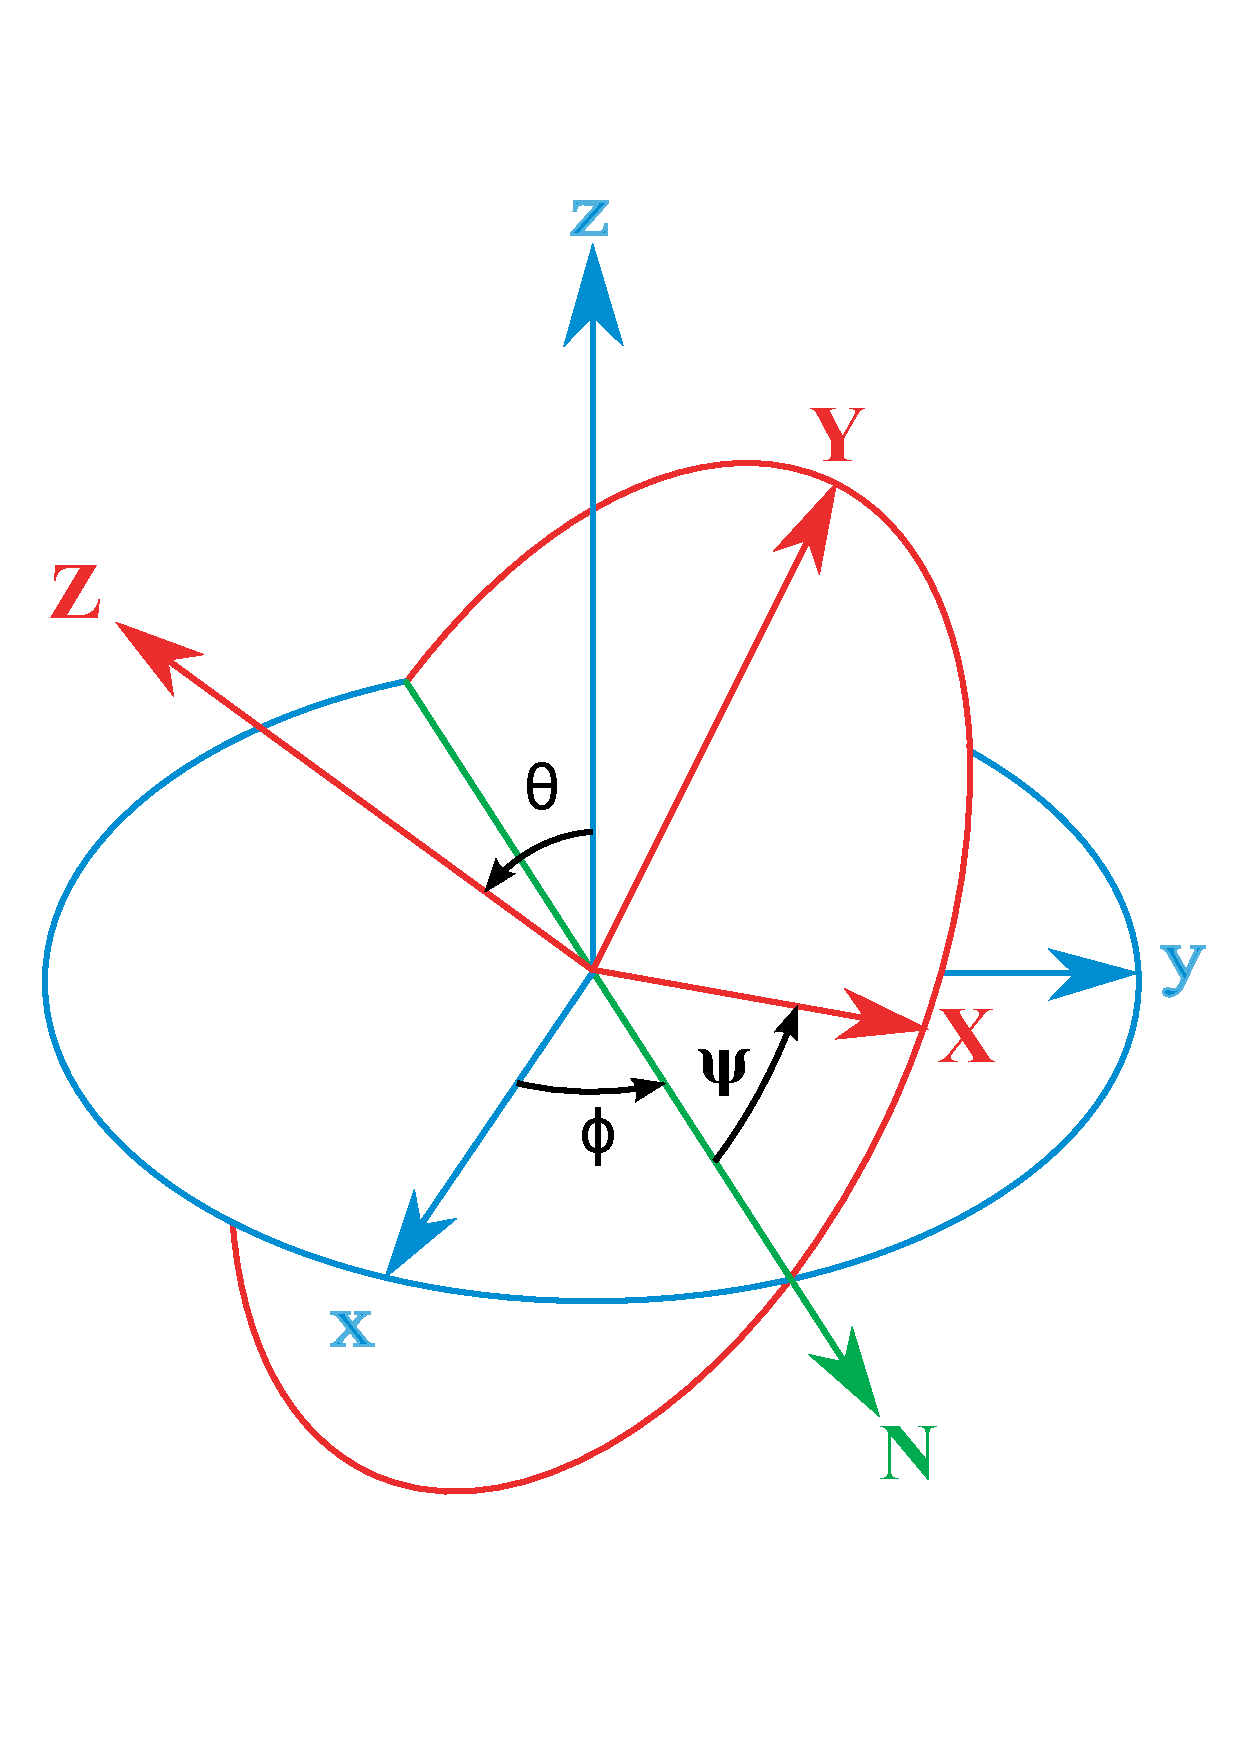
\includegraphics[width=0.25\linewidth]{Eulerangles2.pdf}
    
    \label{fig:enter-label}
\end{figure}

\begin{defn}[Atto di moto]
    L'atto di moto di un sistema rigido a un istante $t$ è il campo delle velocità istantanee, ovvero è $P(t)\mapsto \bv{v}(P(t))$
\end{defn}

\begin{myboxed}
\begin{thm}[teorema di Poisson]
\label{thm:teorema-Poisson}Per ogni \nameref{def:atto-di-moto}
rigido $\exists!\omega=\omega\left(t\right)$ tale che $\forall\boldsymbol{e}$
versore \underline{solidale a $\Sigma'$ con $O'\equiv O$}, vale $$\frac{d[\boldsymbol{e}]_{\Sigma}}{dt}=\boldsymbol{\omega}\times[\boldsymbol{e}]_{\Sigma'}$$
Quindi in generale vale che  $\forall\boldsymbol{W}$
\underline{vettore qualunque di modulo costante solidale con $\Sigma'$}, vale $$\frac{d[\boldsymbol{W}]_{\Sigma}}{dt}=\boldsymbol{\omega}\times[\boldsymbol{W}]_{\Sigma'}$$
\end{thm}
\end{myboxed}

\begin{proof}
Presa $\Sigma'=\left\{ O,\boldsymbol{e}'_{1},\boldsymbol{e}'_{2},\boldsymbol{e}'_{3}\right\} $
terna \underline{ortonormale} solidale con $S$, dimostrando esistenza e unicità
\begin{itemize}
\item[\noun{$!$}] \noun{} Se esistesse anche $\boldsymbol{\omega}'$, allora $0=\frac{d\boldsymbol{e}}{dt}-\frac{d\boldsymbol{e}}{dt}=\left(\boldsymbol{\omega}-\boldsymbol{\omega}'\right)\times\boldsymbol{e} \iff
\boldsymbol{\omega}=\boldsymbol{\omega}'$ in quanto il prod. vettoriale non può annullarsi per parallelismo, dato che deve valere $\forall\bv{e}$
\item[\noun{$\exists$}] \noun{} Vale che $\left(\frac{d}{dt}\boldsymbol{e}'_{i}\right)\cdot\boldsymbol{e}'_{i}=0$,
quindi possiamo supporre che esistono tre vettori $\bv{\omega}_1,\bv{\omega}_2,\bv{\omega}_3$ tali che $$\frac{d}{dt}\boldsymbol{e}'_{i}=\boldsymbol{\omega}_{i}\times\boldsymbol{e}'_{i} \qquad i=1,2,3$$
Ricordiamo l'equazione vettoriale: $x\times a=b \implies
x=\frac{\left(a\times b\right)}{a^{2}}+\lambda a, \quad\lambda\in\re
$, quindi $\bv{x}\cdot \bv{a}=\lambda\abs{\bv{a}}^2$ è arbitraria (infatti conta l'area del parallelogramma compreso, che può essere storto quanto voglio a parità di area). Quindi le componenti $\boldsymbol{\omega}_{i}\cdot\boldsymbol{e}'_{i}$
sono arbitrarie. Impongo allora $$\begin{cases}
\overset{\text{posso sceglierla}}{\boxed{\boldsymbol{\omega}_{1}\cdot\boldsymbol{e}'_{1}}}\coloneqq\boldsymbol{\omega}_{2}\cdot\boldsymbol{e}'_{1} \qquad\text{stesse comp. su $\boldsymbol{e}'_{1}$}\\  
\overset{\text{posso sceglierla}}{\boxed{\boldsymbol{\omega}_{2}\cdot\boldsymbol{e}'_{2}}}\coloneqq
\boldsymbol{\omega}_{1}\cdot\boldsymbol{e}'_{2}\qquad\text{stesse comp. su $\boldsymbol{e}'_{2}$}
\end{cases}$$ 
e da $\boldsymbol{e}'_{1}\cdot\boldsymbol{e}'_{2}=0$ ottengo
\begin{align*}
0 &=\frac{d}{dt}\left(\boldsymbol{e}'_{1}\cdot\boldsymbol{e}'_{2}\right)=\left(\frac{d}{dt}\boldsymbol{e}'_{1}\right)\cdot\boldsymbol{e}'_{2}+\boldsymbol{e}'_{1}\cdot\left(\frac{d}{dt}\boldsymbol{e}'_{2}\right)  \\
&=\left(\boldsymbol{\omega}_{1}\times\boldsymbol{e}'_{1}\right)\cdot\boldsymbol{e}'_{2}+\boldsymbol{e}'_{1}\cdot\left(\boldsymbol{\omega}_{2}\times\boldsymbol{e}'_{2}\right)\\
&\overset{\star}{=}\boldsymbol{\omega}_{1}\cdot\underbrace{\left(\boldsymbol{e}'_{1}\times\boldsymbol{e}'_{2}\right)}_{=\bv{e}_3'}-\underbrace{\left(\boldsymbol{e}'_{1}\times\boldsymbol{e}'_{2}\right)}_{=\bv{e}_3'}\cdot\boldsymbol{\omega}_{2} \qquad\text{prod. misto}\\
\implies\boldsymbol{\omega}_{1}\cdot\boldsymbol{e}'_{3}=\boldsymbol{e}'_{3}\cdot\boldsymbol{\omega}_{2}&\implies\boxed{\boldsymbol{\omega}_{1}=\boldsymbol{\omega}_{2}=\boldsymbol{\omega}}
\end{align*}

dove in $\star$ prodotto  misto è  invariante per permutazione circolare dei fattori e prodotto vettoriale è antisimmetrio. \\
Per l'arbitrarietà della componente imponendo $\boldsymbol{\omega}_{3}\cdot\boldsymbol{e}'_{3}\coloneqq\boldsymbol{\omega}\cdot\boldsymbol{e}'_{3}$,
analogamente  da $\boldsymbol{e}'_{2}\cdot\boldsymbol{e}'_{3}=0$ si ricava che $\boldsymbol{\omega}\cdot\boldsymbol{e}'_{1}=\boldsymbol{e}'_{1}\cdot\boldsymbol{\omega}_{3}$
e $\boldsymbol{\omega}\cdot\boldsymbol{e}'_{2}=\boldsymbol{e}'_{2}\cdot\boldsymbol{\omega}_{3}$,
da cui $\boxed{\boldsymbol{\omega}_{3}=\boldsymbol{\omega}}$ \\
Per vedere che vale $$\frac{d[\boldsymbol{W}]_{\Sigma'}}{dt}=\boldsymbol{\omega}\times[\boldsymbol{W}]_{\Sigma'}$$
basta notare che
\begin{itemize}
    \item $\frac{d[\boldsymbol{W}]_{\Sigma'}}{dt}=\abs{\bv{W}}\frac{d[\boldsymbol{e}]_{\Sigma'}}{dt}$ (linearità derivata)
    \item $\boldsymbol{\omega}\times[\boldsymbol{W}]_{\Sigma'}=\abs{\bv{W}}(\boldsymbol{\omega}\times[\boldsymbol{e}]_{\Sigma'})$ (bilinearità prodotto vettoriale)
\end{itemize}
\end{itemize}
\end{proof}

\begin{lem*}[Spazio tangente delle matrici ortogonali]
    Si ha che lo spazio tangente a quello delle matrici ortogonali $3\times3$, ovvero $SO(3)$, in corrispondenza della matrice identità è lo spazio delle matrici $3\times3$ antisimmetriche, denominato con $so(3)$. 
    $$\mathcal{T}_ISO(3)=so(3)$$
\end{lem*}
\begin{proof}
    \url{https://math.stackexchange.com/questions/2778210/tangent-space-of-orthogonal-matrix}
\end{proof}

\begin{rem*}
    Il teorema di Poisson è conseguenza del teorema appena citato, in quanto 
    \begin{itemize}
        \item $\frac{d\boldsymbol{e}}{dt}=\dot{A}(0)\bv{e}$ con $A(0)=I$ e $A\in SO(3)$ quindi $\dot{A}(0)\in\mathcal{T}_ISO(3)$
        \item $\bv{\omega}\times\bv{e}=\Omega \bv{e}$ con $\Omega\in  so(3)$ poiché le matrici antisimm. $3\times 3$ rappresentano prodotto vettoriale
    \end{itemize}
\end{rem*}

\begin{myboxed}
\begin{cor}[formula fondamentale della cinematica rigida]
Il campo di velocità di un moto rigido è $$\boldsymbol{v}\left(P\right)=\boldsymbol{v}\left(O'\right)+\boldsymbol{\omega}\times\left(P-O'\right)$$
con $O'$ punto prescelto \textbf{solidale} e $\boldsymbol{\omega}$ detta velocità di
rotazione
\end{cor}
\end{myboxed}
\begin{proof}
    Applicare teo. Poisson a $\bv{W}\coloneqq(P-O')$ solidale col corpo e di modulo costante: 
   $$\frac{d}{dt}(P-O')=\boldsymbol{\omega}\times\left(P-O'\right)$$
   e notiamo che $\frac{d}{dt}(P-O')=\frac{d}{dt}[(P-O)-(O'-O)]=\boldsymbol{v}\left(P\right)-\boldsymbol{v}\left(O'\right)$
    
\end{proof}

\begin{defn}[atto di moto traslatorio e moto traslatorio]
Per $\boldsymbol{\omega}\left(t\right)=\boldsymbol{0}$ all'istante
$t$, l'atto di moto è detto traslatorio. Se è traslatorio $\forall t$,
il moto è traslatorio/traslazione.
\end{defn}

\begin{defn}[atto di moto rotatorio e moto rotatorio]
Se $\exists O$ tale che $\boldsymbol{v}_{O}=\boldsymbol{0}$ all'istante
$t$, l'atto di moto è detto rotatorio. Se è rotatorio di centro $O$ $\forall t$,
il moto è una rotatorio/rotazione.
\end{defn}

\begin{prop}[asse istantaneo di moto]
\label{prop:asse-istantaneo-moto}Se $\boldsymbol{\omega}\left(t\right)\neq0$,
esiste una retta parallela a $\boldsymbol{\omega}$ detta asse istantaneo
del moto i cui punti hanno velocità parallela a $\boldsymbol{\omega}$
o nulla. (pensare a \hl{moto di una vite}). \\
Riformulazione: il luogo dei punti che hanno velocità parallela o nulla a $\bv{\omega}$ è almeno una retta.
\end{prop}

\begin{proof}
Analogamente alla costruzione dell'\nameref{prop:asse-centrale} $\left(P-O\right)=\frac{\boldsymbol{\omega}\times\boldsymbol{v}_{O}}{\boldsymbol{\omega}^{2}}+\lambda\boldsymbol{\omega}$.\\
Cerchiamo il luogo dei punti in cui $\bv{v}_P\times\bv{\omega}=\bv{0}$. \\
Da formula fondamentale della cinematica rigida:
\begin{align*}
   \boldsymbol{\omega}\times\left(P-O\right)=\boldsymbol{v}\left(P\right)-\boldsymbol{v}\left(O\right)\\
   \implies  \left(P-O\right)\times\boldsymbol{\omega}=\boldsymbol{v}\left(O\right)-\boldsymbol{v}\left(P\right)
\end{align*}
e ricordando l'equazione vettoriale: $x\times a=b \implies
x=\frac{\left(a\times b\right)}{a^{2}}+\lambda a, \quad\lambda\in\re
$, abbiamo 
$$\left(P-O\right)=\frac{\boldsymbol{\omega}\times(\boldsymbol{v}_{O}-\bv{v}_P)}{\boldsymbol{\omega}^{2}}+\lambda\boldsymbol{\omega} \quad \lambda\in\re$$
quindi se cerchiamo i punti tali che $\bv{v}_P\times\bv{\omega}=\bv{0}$ abbiamo
$$\left(P-O\right)=\frac{\boldsymbol{\omega}\times\boldsymbol{v}_{O}}{\boldsymbol{\omega}^{2}}+\lambda\boldsymbol{\omega}  \quad \lambda\in\re$$
quindi se $\bv{v}_O=0$ oppure parallela a $\bv{\omega}\implies(P-O)=\lambda\bv{\omega}, \;\lambda\in\re$ retta che soddisfa le richieste.
\end{proof}


\begin{rem*}
    Non confondere asse istantaneo di moto con asse di rotazione: ad esempio, in una ruota che rotola l'asse di rotazione è il centro della ruota, mentre l'asse istantaneo di moto è nel punto di contatto col terreno, infatti è come se istantaneamente la ruota si stesse muovendo di pura rotazione attorno a questo punto. Vediamo infatti che il punto di contatto ha velocità nulla rispetto  a tale asse. Se la ruota si muovesse anche in direzione uscente dal foglio allora l'asse istantaneo di moto rimane il punto di contatto, che però ha una componente della velocità parallela all'asse.
\end{rem*}

\begin{defn}[invariante rigido]
\label{def:invariante-rigido}$J=\boldsymbol{v}_{P}\cdot\boldsymbol{\omega}$,
agisce similmente a $I$ definito in \ref{def:invariante-momento}. È invariante , infatti 
$$\bv{v}_P=\bv{v}_O+\bv{\omega}\times(P-O)\implies \bv{v}_P\cdot\bv{\omega}=\bv{v}_O\cdot\bv{\omega} \quad\forall P$$
dove $O$ è un punto prescelto solidale.
\end{defn}

Preso l'\nameref{def:invariante-rigido} $J$ posso avere
\begin{center}
\begin{tabular}{ccc}
\multicolumn{2}{c}{$J=0$} & $J\neq0$\tabularnewline
Moto traslatorio & Moto rotatorio & Moto elicoidale\tabularnewline
{\footnotesize{}$\boldsymbol{\omega}\left(t\right)=\boldsymbol{0}$} & {\footnotesize{}$\boldsymbol{\omega}\left(t\right)\neq\boldsymbol{0}$} & \tabularnewline
\end{tabular}
\par\end{center}





Per $\boldsymbol{\omega}\left(t\right)\neq\boldsymbol{0}$ esiste
l'\nameref{prop:asse-istantaneo-moto} che per il moto rotatorio ($J=0$)
è formato dai punti di velocità nulla.




\begin{thm}[teorema di Mozzi]
A un dato istante $t$, l'atto di moto di un sistema rigido è traslatorio, rotatorio oppure elicoidale. 
\end{thm}


\subsection{Moti rigidi piani}
\begin{defn}[moto rigido piano]
Le velocità di tutti i punti sono parallele a $\pi$, piano fisso
rispetto al riferimento $\Sigma$.
\end{defn}
\begin{rem*}
    praticamente sono tutti i moti (rotatorio e traslatorio) \textbf{tranne quello elicoidale}, ovvero non ammetto che ci sia componente di traslazione nella direzione di $\bv{\omega}$
\end{rem*}

\begin{prop} Il moto piano ha le seguenti proprietà:
\begin{enumerate}
    \item $\boldsymbol{\omega}$ è perpendicolare a $\pi$ o è nullo, ovvero
$\boldsymbol{\omega}\left(t\right)=\omega\left(t\right)\boldsymbol{e}$
con $\boldsymbol{e}$ versore $\perp\pi$ 
\item L'atto di moto è in ogni istante traslatorio o rotatorio. Infatti,
se $\boldsymbol{\omega}\left(t\right)\neq\boldsymbol{0}$, preso $P^{*}$
appartenente all'\nameref{prop:asse-istantaneo-moto} vale $\boldsymbol{v}\left(P^{*}\right)=\boldsymbol{0}$,
essendo impossibile $\boldsymbol{v}\left(P^{*}\right)\parallel\boldsymbol{\omega}$.
\item Posso studiare il sistema prendendo $p$ piano rappresentativo parallelo
a $\pi$ e solidale a $S$
\end{enumerate}
    
\end{prop}


\begin{defn}[centro di istantanea rotazione]
$C$ intersezione tra l'\nameref{prop:asse-istantaneo-moto} e il
piano $p$. 
\end{defn}

\begin{rem*}
    Il centro istantaneo di rotazione è l'unico punto che, istante per istante, ha velocità nulla
\end{rem*}

\begin{prop}[Criterio di Chasles per l'individuazione del centro ist. di rotazione]
    
\end{prop}





\subsection{Vincoli di contatto}
\begin{defn}[vincolo di contatto]
\label{def:vincolo-contatto}$\mathcal{C}_{1},\mathcal{C}_{2}$ sistemi
rigidi a contatto in un punto $P$, il vincolo di contatto è espresso
da $\left(\boldsymbol{v}_{1}-\boldsymbol{v}_{2}\right)\cdot\boldsymbol{n}=0$
con $\boldsymbol{v}_{i}$ velocità del punto di $\mathcal{C}_{i}$
coincidente con $P$ e $\boldsymbol{n}$ normale alla tangente in
$P$.
\end{defn}

\begin{defn}[rotolamento senza strisciamento]
Caso di \nameref{def:vincolo-contatto} con $\boldsymbol{v}_{1}=\boldsymbol{v}_{2}$.
\end{defn}

\subsection{Velocità angolare in funzione degli angoli di Eulero}
\begin{prop}
    Vale $\bv{\omega}(t)=\dot{\varphi}\bv{e}_3+\dot{\theta}\bv{n}+\dot{\psi}\bv{e}_3'$
\end{prop}

\begin{lem*}
    $[\dot{\bv{u}}]_\Sigma=[\dot{\bv{u}}]_{\Sigma'}+\bv{\omega}\times\bv{u}$
\end{lem*}

\begin{prop}
    $\bv{\omega}(t)=\omega_1\bv{e}_1'+\omega_2\bv{e}_2'+\omega_3\bv{e}_3'$ con
    \begin{itemize}
        \item $\omega_1=[\dots]$
        \item $\omega_2=[\dots]$
        \item $\omega_3=[\dots]$
    \end{itemize}
\end{prop}

\begin{xca*}[velocità angolare mediante gli \nameref{def:angoli-Eulero}]
Preso $O\equiv O'$ vale che $\boldsymbol{\omega}=\dot{\varphi}\boldsymbol{k}+\dot{\theta}\boldsymbol{n}+\dot{\psi}\boldsymbol{k}'$,
siccome

\begin{align*}
\left(\dot{\boldsymbol{i}'}\right)_{\Sigma} & =\left(\dot{\boldsymbol{i}'}\right)_{\Sigma_{1}}+\omega_{\Sigma,\Sigma_{1}}\times\boldsymbol{i} & \left(\dot{\boldsymbol{i}'}\right)_{\Sigma_{1}} & =\left(\dot{\boldsymbol{i}'}\right)_{\Sigma_{2}}+\omega_{\Sigma_{1},\Sigma_{2}}\times\boldsymbol{i} & \left(\dot{\boldsymbol{i}'}\right)_{\Sigma_{2}} & =\cancel{\left(\dot{\boldsymbol{i}'}\right)_{\Sigma'}}+\omega_{\Sigma_{2},\Sigma'}\times\boldsymbol{i}
\end{align*}
\[
\left(\dot{\boldsymbol{i}'}\right)_{\Sigma}=\left(\omega_{\Sigma,\Sigma_{1}}+\omega_{\Sigma_{1},\Sigma_{2}}+\omega_{\Sigma_{2},\Sigma'}\right)\times\boldsymbol{i}=\left(\dot{\varphi}\boldsymbol{k}+\dot{\theta}\boldsymbol{n}+\dot{\psi}\boldsymbol{k}'\right)\times\boldsymbol{i}\overset{\text{\nameref{thm:teorema-Poisson}}}{=}\boldsymbol{\omega}\times\boldsymbol{i'}
\]

L'espressione invece nella terna solidale $\left(\boldsymbol{i}',\boldsymbol{j}',\boldsymbol{k}'\right)$
viene essere
\[
\boldsymbol{\omega}=+\dot{\psi}\boldsymbol{k}'+\dot{\theta}\left(\boldsymbol{i}'\cos\psi-\boldsymbol{j}'\sin\psi\right)+\dot{\varphi}\left(\boldsymbol{k}'\cos\theta+\left(\boldsymbol{i}'\cos\left(\frac{\pi}{2}-\psi\right)+\boldsymbol{j}'\cos\psi\right)\sin\theta\right)
\]
\end{xca*}
%
\begin{xca*}[equazioni di Lagrange in un riferimento in moto rotatorio uniforme]
{[}...{]}
\end{xca*}



\pagebreak{}

\section{Moti Relativi}
\subsection{Cinematica relativa}

$\Sigma=\left\{ O,\boldsymbol{i},\boldsymbol{j},\boldsymbol{k}\right\} $
riferimento inerziale (assoluto) e $\Sigma'=\left\{ O',\boldsymbol{i}',\boldsymbol{j}',\boldsymbol{k}'\right\} $
riferimento in moto rispetto a $\Sigma$, le cui misure sono dette
assolute e relative rispettivamente, e di trascinamento quelle dovute
al movimento di $O'$ rispetto a $O$.
\paragraph{Derivata assoluta e relativa}
Sia $\bv{u}(t)$ vettore che \underline{si muove (quindi non solidale) in $\Sigma'$ con $O\equiv O'$}
\begin{itemize}
    \item Derivata assoluta: in $\Sigma$: $\bv{u}(t)=\sum_iu_i(t)\bv{e}_i$ e  $[\dot{\bv{u}}(t)]_\Sigma=\sum_i\dot{u}_i(t)\bv{e}_i$
    \item Derivata relativa: in $\Sigma'$: $\bv{u}(t)=\sum_iu_i'(t)\bv{e}_i'$ e  $[\dot{\bv{u}}(t)]_{\Sigma'}=\sum_i\dot{u}_i'(t)\bv{e}_i'$
\end{itemize}
Quindi derivando $[\bv{u}(t)]_{\Sigma'}$ in $\Sigma$ otteniamo:
$$[\dot{\bv{u}}]_\Sigma=\sum_i\dot{u}_i'(t)\bv{e}_i'(t)+\sum_iu_i'(t)\underbrace{\dot{\bv{e}}_i'}_{\text{\textcolor{red}{Teo.Poisson }}=\bv{\omega}\times\bv{e}_i'}=[\dot{\bv{u}}]_{\Sigma'}+\bv{\omega}\times\underbrace{\sum_iu_i'\bv{e}_i'}_{\bv{u}(t)}=[\dot{\bv{u}}]_{\Sigma'}+\bv{\omega}\times[\bv{u}]_{\Sigma'}$$
Quindi abbiamo, per un vettore qualcunque $\bv{u}$:
$$\boxed{[\dot{\bv{u}}]_\Sigma=[\dot{\bv{u}}]_{\Sigma'}+\bv{\omega}\times[\bv{u}]_{\Sigma'}}$$
È \textbf{generalizzazione del teorema di Poisson}, infatti non vale solo per vettori di modulo costante e solidali, ma per tutti.


\begin{thm}[composizione delle velocità e accelerazioni] Si ha: \\
Per $O'\equiv O$:
\begin{enumerate}
    \item $[{\bv{v}}]_\Sigma=\overset{\bv{v}_{\text{relativa}}}{\boxed{[{\bv{v}}]_{\Sigma'}}}+\overset{\bv{v}_{\text{trascinamento}}}{\boxed{{\bv{\omega}\times(P-O')}}}$
    \item $[{\bv{a}}]_\Sigma=\overset{\bv{a}_{\text{relativa}}}{\boxed{[{\bv{v}}]_{\Sigma'}}}+\overset{\bv{a}_{\text{coriolis}}}{\boxed{2\bv{\omega}\times[\bv{v}]_{\Sigma'}}}+\overset{\bv{a}_{\text{trascinamento}}}{\boxed{\dot{\bv{\omega}}\times(P-O')+\bv{\omega}\times(\bv{\omega}\times(P-O'))}}$

\end{enumerate}
Per $O'\not\equiv O$
\begin{enumerate}
\item $[{\bv{v}}]_\Sigma=\overset{\bv{v}_{\text{relativa}}}{\boxed{[{\bv{v}}]_{\Sigma'}}}+\overset{\bv{v}_{\text{trascinamento}}}{\boxed{{\bv{\omega}\times(P-O')}+\textcolor{blue}{\bv{v}(O')}}}$
    \item $[{\bv{a}}]_\Sigma=\overset{\bv{a}_{\text{relativa}}}{\boxed{[{\bv{v}}]_{\Sigma'}}}+\overset{\bv{a}_{\text{coriolis}}}{\boxed{2\bv{\omega}\times[\bv{v}]_{\Sigma'}}}+\overset{\bv{a}_{\text{trascinamento}}}{\boxed{\dot{\bv{\omega}}\times(P-O')+\bv{\omega}\times(\bv{\omega}\times(P-O'))+\textcolor{blue}{\bv{a}(O')}}}$
\end{enumerate}
\end{thm}

\begin{proof}
Assumo $O'\equiv O$ a cui poi basta aggiungere $\boldsymbol{v}\left(O'\right)$
e $\boldsymbol{a}\left(O'\right)$. Per la velocità è la semplice applicazione della derivata di un qualunque vettore vista sopra, mentre per l'accelerazione:
\begin{align*}
\boldsymbol{a}_{a}=[\dot{\bv{v}}]_{\Sigma}&=\left[\frac{d}{dt}(\bv{v}_r+\bv{\omega}\times(P-O))\right]_{\Sigma'}+\bv{\omega}\times[\bv{v}_r+\bv{\omega}\times(P-O)] \\
&= \left[\frac{d}{dt}\bv{v}_r\right]_{\Sigma'}+\dot{\bv{\omega}}\times(P-O')+\bv{\omega}\times\underbrace{\frac{d}{dt}(P-O')}_{\bv{v}_r}+\bv{\omega}\times\bv{v}_r+\bv{\omega}\times(\bv{\omega}\times(P-O')) \\
&=\bv{a}_r+2\bv{\omega}\times\bv{v}_r+\dot{\bv{\omega}}\times(P-O')+\bv{\omega}\times(\bv{\omega}\times(P-O'))
\end{align*}
\end{proof}

\begin{rem*}
    $\bv{a}_c=0 \iff\bv{\omega}(t)=\bv{0}$ (moto traslatorio) oppure $\bv{v}_r=\bv{0}$ (oggetto fermo rispetto a $\Sigma')$. Inoltre la potenza della forza di Coriolis è zero perché è perpendicolare alla velocità relativa.
\end{rem*}

\begin{example*}[moto rotatorio uniforme]
$\omega=\text{cost}$, $\dot{\omega}=0$
\begin{align*}
\boldsymbol{a}_{t} &=\cancel{\dot{\boldsymbol{\omega}}\times\left(P-O'\right)}+\boldsymbol{\omega}\times\left[\boldsymbol{\omega}\times\left[\left(P-P^{*}\right)+\overset{\parallel\omega}{\left(P^{*}-O'\right)}\right]\right] \quad \text{$P^*\in$ asse istantaneo di moto}  \\
&=-\left[\boldsymbol{\omega}\times\left(P-P^{*}\right)\right]\times\boldsymbol{\omega}\\
 &=-\left[\boldsymbol{\omega}^{2}\left(P-P^{*}\right)-\bcancel{\left(\left(P-P^{*}\right)\cdot\boldsymbol{\omega}\right)}\cdot\boldsymbol{\omega}\right] \\
 &=-\boldsymbol{\omega}^{2}\left(P-P^{*}\right) \quad\longrightarrow \text{accelerazione centripeta}
\end{align*}
\end{example*}

\subsection{Dinamica relativa}
Per quanto riguarda l'interpretazione dinamica vale $\left(m\boldsymbol{a}_{r}\right)_{\Sigma'}=\boldsymbol{F}-m\boldsymbol{a}_{c}-m\boldsymbol{a}_{t}$
\begin{align*}
    \text{In }&\Sigma:\quad m\bv{a}_a=\bv{F} \\
    \text{In }&\Sigma':\quad m(\bv{a}_r+\bv{a}_c+\bv{a}_t)=\bv{F} \implies m\bv{a}_r=\bv{F}\underbrace{-m\bv{a}_c-m\bv{a}_t}_{\text{forze apparenti}} \coloneqq \widetilde{\bv{F}}\\
\end{align*}
dove
\begin{itemize}
    \item $\bv{F}_c=-m\bv{a}_c=-2m\bv{\omega\times\bv{v}_r}$ (forza di Coriolis)
    \item $\bv{F}_t=-m\bv{a}_t$ (forza di trascinamento)
    \item $\widetilde{\bv{F}}=\bv{F}+\bv{F}_c+\bv{F}_t$
\end{itemize}

%
\begin{xca*}[effetto Coriolis]
$m\boldsymbol{a}_{r}=\boldsymbol{F}-m\boldsymbol{a}_{c}-m\boldsymbol{a}_{t}$
con $\boldsymbol{F}-m\boldsymbol{a}_{t}\overset{\text{def}}{=}m\boldsymbol{g}\approx\boldsymbol{F}$,
da cui $m\boldsymbol{a}_{r}=m\boldsymbol{g}-2m\boldsymbol{\omega}\times\boldsymbol{v}_{r}$,
da cui (con $\varphi$ latitudine di $O'$ sulla superficie terrestre,
$\boldsymbol{k}'$ Zenith, $\boldsymbol{i}'$ verso est, $\boldsymbol{j}'$
verso sud, $P=\left(0,0,h\right)_{\Sigma'}$ di velocità iniziale
nulla)
\begin{align*}
 & \begin{cases}
\ddot{x'}_{1}=2\boldsymbol{\omega}\left(\cos\varphi\dot{x'}_{3}+\sin\varphi\dot{x'}_{2}\right)\\
\ddot{x'}_{2}=-2\boldsymbol{\omega}\sin\varphi\dot{x'}_{1}\\
\ddot{x'}_{3}=-2\boldsymbol{\omega}\cos\varphi\dot{x'}_{1}-g
\end{cases} & \text{risolvendo \ensuremath{\Longrightarrow} } & \begin{cases}
x'_{1}=\frac{\cos\varphi g}{2\boldsymbol{\omega}}\left(\frac{\sin\left(2\omega t\right)}{2\boldsymbol{\omega}}-t\right)\overset{\text{Taylor}}{\simeq}-\frac{1}{3}\cos\varphi g\omega t^{3}\\
x'_{2}=\text{[...]}\\
x'_{3}=\text{[...]}
\end{cases}
\end{align*}
\end{xca*}


\begin{rem*}
    Dato che     $[\dot{\bv{u}}]_\Sigma=[\dot{\bv{u}}]_{\Sigma'}+\bv{\omega}\times\bv{u} \implies [\dot{\bv{\omega}}]_\Sigma=[\dot{\bv{\omega}}]_{\Sigma'}+\cancel{\bv{\omega}\times\bv{\omega}}$ per questo non specifico se $\dot{\bv{\omega}}$ rel o ass. \\
    Ogni vettore della forma $\bv{u}(t)=\lambda(t)\bv{\omega}(t)$ gode della proprietà $[\dot{\bv{u}}]_\Sigma=[\dot{\bv{u}}]_{\Sigma'}$
\end{rem*}

\subsection{Equazioni di Lagrange in sistema di riferimento rotatorio uniforme}
\begin{itemize}
    \item Forza relativa di \textbf{trascinamento} è conservativa di potenziale $$V_t=-\frac{1}{2}m\omega^2d^2=-\frac{1}{2}\omega^2\mathcal{I}_r$$ 
   
    con $\omega$ la vvelocità angolare del sistema di riferimento e $d$ la distanza dall'asse di rotazione. Per un corpo esteso
     $$V_t=-\frac{1}{2}\omega^2\int\int\int\rho(\bv{x})d(\bv{x})^2d\bv{x}$$
    \item Forza di \textbf{Coriolis} non interviene in eq. di Lagrange perché ha componente lagrangiana nulla
\end{itemize}
Allora per $N$ punti
$$ \mathcal{L}'=\sum_N T'-\sum_N V'-\sum_N V_t$$
con $T',V'$ sono valutate nel sistema di riferimento rotante


\pagebreak{}

\section{Dinamica dei sistemi rigidi}
\subsection{Geometria delle masse}

$S$ sistema discreto di punti materiali di centro di massa
$G=O+\frac{\sum m_{i}\left(P_{i}-O\right)}{\sum m_{i}}$, massa totale
$M=\sum m_{i}$

\begin{defn}[Centro di massa] Distinguiamo i casi
\begin{itemize}
    \item \textbf{Sistema discreto}
    \begin{align*}
        S=\{(P_i,m_i),\quad i=1\dots N\} & & M=\sum m_i & & \bv{R}=\frac{\sum m_{i}\left(P_{i}-O\right)}{\sum m_{i}}
    \end{align*}
    \item \textbf{Sistema continuo}
    \begin{align*}
        S=\{(P,\rho(P)),\quad P\in \mathbb{E}\} & & M=\int_S \rho(P)dS & & \bv{R}=\frac{\int_S \rho(P)\left(P-O\right)dS}{M}
    \end{align*}
\end{itemize}
    
\end{defn}

\begin{defn}[momento d'inerzia]
\label{def:momento-inerzia}$\mathcal{I}_{r}=\sum m_{i}d_{i}^{2}=\sum m_{i}\left[\left(P_{i}-O\right)\times\boldsymbol{n}\right]^{2}$
Momento d'inerzia rispetto alla retta $r$ ($\boldsymbol{n}$ versore
di $r$. $d_i$ distanza di $P_i$ dalla retta $r$)
\end{defn}

\begin{thm}[teorema di Huygens (variazione in fascio improprio)]
\label{thm:teorema-Huygens}$\mathcal{I}_{r}=\mathcal{I}_{r'}+Md^{2}$
con $r'\parallel r$ passante per $G$
\end{thm}

\begin{proof}
Preso $G$ centro di massa e $\left(P_{i}-O\right)=\left(P_{i}-G\right)+\left(G-O\right)=\bv{r}_i'+\bv{R}$
\begin{align*}
\mathcal{I}_{r} &=\sum_im_i[(\bv{r}_i'+\bv{R})\times\bv{n}]^2=\sum_im_i((\bv{r}_i'\times\bv{n})+(\bv{R}\times\bv{n}))^2 \\
&=\underbrace{\sum_im_i(\bv{r}_i'\times\bv{n})^2}_{\mathcal{I}_{\bv{r'}}}+\underbrace{\sum_im_i(\bv{R}\times\bv{n})^2}_{Md^2}+\underbrace{2\sum_im_i(\bv{r}_i'\times\bv{n})(\bv{R}\times\boldsymbol{n})}_{=0}
\end{align*}
dove l'ultimo termine è nullo poiché:
$$2\sum_im_i(\bv{r}_i'\times\bv{n})(\bv{R}\times\boldsymbol{n})=2(\bv{R}\times\boldsymbol{n})\sum_im_i(\bv{r}_i'\times\bv{n})=2(\bv{R}\times\boldsymbol{n})[\underbrace{(\sum_im_i\bv{r}_i')}_{=M(G-G)=0}\times\bv{n}]=0$$

\end{proof}
\begin{defn}[prodotto di inerzia] 
\label{def:prodotto-inerzia} rispetto ad una coppia di piani $\pi,\pi'$ non paralleli: $$\mathcal{I}_{\pi,\pi'}\coloneqq-\sum m_{i}\left[\left(P_{i}-O\right)\cdot\boldsymbol{n}\right]\left[\left(P_{i}-O\right)\cdot\boldsymbol{n}'\right]=-\sum m_id_{r}d_{r'}$$
con $\boldsymbol{n},\boldsymbol{n}'$ versori perpendicolari a $\pi,\pi'$ rispettivamente e $O\in\pi\cap\pi'$

\end{defn}

\begin{rem*}
Per $\boldsymbol{n}=\boldsymbol{i}$ e $\boldsymbol{n}'=\boldsymbol{k}$
vale $\mathcal{I}_{x,z}\coloneqq\mathcal{I}_{\pi,\pi'}=-\sum m_{i}x_{i}z_{i}$ poiché \hl{distanza dal piano $Oyz$ perpendicolare ad asse $x$ è la coordinata $x$}
\end{rem*}

\begin{myboxed}
\begin{thm}[variazione del \nameref{def:momento-inerzia} in un fascio proprio] Presa retta $r$ per $O$, assi \underline{cartesiani} $x,y,z$ solidali, $\bv{n}=\alpha\bv{u}_x+\beta\bv{u}_y+\gamma\bv{u}_z$ versore (quindi $\alpha^2+\beta^2+\gamma^2=1$ sono i coseni direttori) della retta nella base solidale, allora
$$\mathcal{I}_{r}=\mathcal{I}_{r}\left(\alpha,\beta,\gamma\right)=\alpha^{2}\mathcal{I}_{x,x}+\beta^{2}\mathcal{I}_{y,y}+\gamma^{2}\mathcal{I}_{z,z}+2\alpha\beta\mathcal{I}_{x,y}+2\beta\gamma\mathcal{I}_{y,z}+2\alpha\gamma\mathcal{I}_{x,z}$$
ovvero
$$\mathcal{I}_{r}=\left(\alpha,\beta,\gamma\right)\begin{pmatrix}\mathcal{I}_{x,x} & \mathcal{I}_{x,y} & \mathcal{I}_{x,z}\\
\mathcal{I}_{y,x} & \mathcal{I}_{y,y} & \mathcal{I}_{y,z}\\
\mathcal{I}_{z,x} & \mathcal{I}_{z,y} & \mathcal{I}_{z,z}
\end{pmatrix}\begin{pmatrix}\alpha\\
\beta\\
\gamma
\end{pmatrix}=\boldsymbol{n}^T I_{O}\boldsymbol{n}$$
dove
\begin{itemize}
\item $\mathcal{I}_r$ è il momento di interzia del sistema rispetto alla retta $r$
    \item $\mathcal{I}_{\square,\square}$ è il momento d'inerzia del sistema rispetto all'asse $\square$
    \item $\mathcal{I}_{\square,\triangle}$ è il prodotto d'inerzia del sistema rispetto ai piani perpendicolari agli assi $\square$ e $\triangle$
\end{itemize}
\end{thm}
\end{myboxed}

\begin{proof}
Preso $G$ centro di massa e $\left(P_{i}-O\right)=\left(P_{i}-G\right)+\left(G-O\right)$
\begin{align*}
\mathcal{I}_{r} & =\sum m_{i}d_{i}^{2}\overset{\star}{=}\sum m_{i}\overset{\text{Pitagora}}{\left[\left(x_{i}^{2}+y_{i}^{2}+z_{i}^{2}\right)-\left(\left(P_{i}-O\right)\cdot\boldsymbol{n}\right)^{2}\right]}=\sum m_{i}\left[\left(x_{i}^{2}+y_{i}^{2}+z_{i}^{2}\right)-\left(\alpha x_{i}+\beta y_{i}+\gamma z_{i}\right)^{2}\right]
\end{align*}
poi conti: prima raccolgo $x_i,y_i,z_i$ poi ricordo che  $\alpha^2+\beta^2+\gamma^2=1$ quindi sostituisco e raccolgo $\alpha,\beta,\gamma$.
\end{proof}
\begin{defn}[Matrice d'inerzia] Matrice d'inerzia rispetto ad $O$:
$I_{O}\coloneqq\begin{pmatrix}\mathcal{I}_{x,x} & \mathcal{I}_{x,y} & \mathcal{I}_{x,z}\\
\mathcal{I}_{y,x} & \mathcal{I}_{y,y} & \mathcal{I}_{y,z}\\
\mathcal{I}_{z,x} & \mathcal{I}_{z,y} & \mathcal{I}_{z,z}
\end{pmatrix}$, allora $$\mathcal{I}_{r}=\left(\alpha,\beta,\gamma\right)I_{0}\begin{pmatrix}\alpha\\
\beta\\
\gamma
\end{pmatrix}=\boldsymbol{n}^T I_{O}\boldsymbol{n}$$
Notiamo che essendo simmetrica è sempre diagonalizzabile mediante matrici ortogonali per il \textbf{teorema spettrale reale}.
\end{defn}
\begin{defn}[ellissoide d'inerzia]
\label{def:ellissoide-inerzia}Per $\mathcal{I}_{r}>0$ considero
$P\in\Sigma$ tali che $d\left(P,O\right)=\frac{1}{\sqrt{\mathcal{I}_{r}}}$
con $P\in r$, quindi i $P=\frac{1}{\sqrt{I_r}}\bv{n}$ di coordinate $\left(\frac{\alpha}{\sqrt{\mathcal{I}_{r}}},\frac{\beta}{\sqrt{\mathcal{I}_{r}}},\frac{\gamma}{\sqrt{\mathcal{I}_{r}}}\right)$,
da cui l'equazione 
\begin{align*}
    \left(x,y,z\right)I_{O}\begin{pmatrix}x\\
y\\
z
\end{pmatrix}=1 \\
x^{2}\mathcal{I}_{x,x}+y^{2}\mathcal{I}_{y,y}+z^{2}\mathcal{I}_{z,z}+2xy\mathcal{I}_{x,y}+2yz\mathcal{I}_{y,z}+2xz\mathcal{I}_{x,z}=1
\end{align*}
si può otterene anche dividendo per $\mathcal{I}_r$ l'ugualianza nel teorema sopra, poi estendo a tutti i punti $(x,y,z)$ e quindi la relazione è soddisfatta solo dai punti $\left(\frac{\alpha}{\sqrt{\mathcal{I}_{r}}},\frac{\beta}{\sqrt{\mathcal{I}_{r}}},\frac{\gamma}{\sqrt{\mathcal{I}_{r}}}\right)$, ovvero dai punti $P=\frac{1}{\sqrt{I_r}}\bv{n}$ che quindi distano $1/\sqrt{\mathcal{I}_r}$ da $O$, con $r$ retta per $P-O$ (variabile punto per punto). È una quadratica (ellissoide, paraboloide, iperboloide), in questo caso è un ellissoide (dato che  $\mathcal{I}_{\square,\square}\ge 0$ e  $\mathcal{I}_{\square,\triangle}\le0$) \textbf{non traslato} (in quanto è forma quadratica e quindi non ha termini di primo o zero grado), ma \textbf{ruotato}.
\end{defn}

Conoscere l'ellissoide permette di ricavare ogni $\mathcal{I}_{r}$,
ed è indipendente da $\Sigma$. Lo cerchiamo nella forma canonica:
\begin{defn}[assi principali, terna principale, terna centrale]\label{def:assi-principali-terna-principale-terna-centrale} Per assi di simmetria si intende non assi di simmetria centrale, ma assi per cui c'è un \textbf{piano} perpendicolare di simmetria
\begin{itemize}
    \item \noun{Assi principali}: assi di simmetria dell'ellissoide;
    \item \noun{Terna principale}:
terna degli assi principali; 
\item \noun{Terna centrale}: terna principale con $O\equiv G$.
\end{itemize}

\end{defn}

\begin{prop}
Una terna è principale $\Longleftrightarrow$ $I_{O}=\begin{pmatrix}\mathcal{I}_{x,x} & 0 & 0\\
0 & \mathcal{I}_{y,y} & 0\\
0 & 0 & \mathcal{I}_{z,z}
\end{pmatrix}$ è diagonale, e dunque l'ellissoide è $$x^{2}\mathcal{I}_{x,x}+y^{2}\mathcal{I}_{y,y}+z^{2}\mathcal{I}_{z,z}=1\quad \text{(ellissoide \textbf{non ruotato}, e non tralsato come al solito)}$$
ovvero gli assi sono principali $\iff$ sono gli \textbf{autospazi} della matrice d'inerzia \\
e la terna è principale $\iff$ è la base in cui la matrice è diagonale
\end{prop}



\subsubsection{Omografia d'inerzia}
È l'operatore lineare associato alla matrice d'inerzia.
\begin{defn}[omografia d'inerzia]
\label{def:omografia-inerzia}è l'applicazione lineare $\sigma\left(O\right)\colon V\rightarrow V$
tale che $$\sigma\left(O\right)\left(\boldsymbol{u}\right)=\sum_{i=1}^{n}m_{i}\left[r_{i}^{2}\boldsymbol{u}-\left(\boldsymbol{r}_{i}\cdot\boldsymbol{u}\right)\boldsymbol{r}_{i}\right]=I_O\bv{u}$$
con $V$ spazio delle traslazioni, con $\bv{u}\in\re^3$ vettore qualunque, $\boldsymbol{r}_{i}=P_{i}-O$
e $r_{i}^{2}=\left|P_{i}-O\right|^{2}$. \\
\end{defn}

\begin{prop}
 L'applicazione $\sigma\left(O\right)$ ha le proprietà:
\end{prop}

\begin{enumerate}
\item $\boldsymbol{v}\cdot\sigma\left(O\right)\left(\boldsymbol{v}\right)=\mathcal{I}_{\boldsymbol{v}}\cdot v^{2}$\qquad{}(con
$\mathcal{I}_{\boldsymbol{v}}\coloneqq\mathcal{I}_{r}$ per $r$ retta
$\parallel\boldsymbol{v}$ passante per $O$)
\item per $\boldsymbol{u},\boldsymbol{v}\in V$ non paralleli, $\boldsymbol{u}\cdot\sigma\left(O\right)\left(\boldsymbol{v}\right)=\mathcal{I}_{\pi_{\boldsymbol{u}},\pi_{\boldsymbol{v}}}\left|\boldsymbol{u}\right|\left|\boldsymbol{v}\right|+\sum_{i}m_{i}r_{i}^{2}\boldsymbol{u}\cdot\boldsymbol{v}$\qquad{}(con
$\pi_{\boldsymbol{u}},\pi_{\boldsymbol{v}}$ perpendicolari a $\boldsymbol{u},\boldsymbol{v}$
rispettivamente, $O\in\pi_{\boldsymbol{u}}\cap\pi_{\boldsymbol{v}}$
\end{enumerate}


\begin{proof}
\begin{align*}
\boldsymbol{v}\cdot\sigma\left(O\right)\left(\boldsymbol{v}\right) & =\sum m_{i}\left[r_{i}^{2}v^{2}-\left(\boldsymbol{r}_{i}\cdot\boldsymbol{v}\right)^{2}\right]=\sum m_{i}\left[r_{i}^{2}v^{2}-r_{i}^{2}v^{2}\cos^{2}\theta\right]=\sum m_{i}\left[r_{i}^{2}v^{2}\sin^{2}\theta\right]=\sum m_{i}\left[\boldsymbol{r}_{i}\times\boldsymbol{v}\right]^{2}\\
&=\sum m_i(\bv{r}_i\times \bv{n}_i)^2v^2=\mathcal{I}_{\bv{n}}v^2 \quad \text{ con }\bv{n}=\frac{\bv{v}}{\norm{\bv{v}}} \\
\boldsymbol{u}\cdot\sigma\left(O\right)\left(\boldsymbol{v}\right) & =\sum m_{i}\left[r_{i}^{2}\left(\boldsymbol{u}\cdot\boldsymbol{v}\right)-\left(\boldsymbol{r}_{i}\cdot\boldsymbol{v}\right)\left(\boldsymbol{r}_{i}\cdot\boldsymbol{u}\right)\right]=\sum m_{i}r_{i}^{2}\left(\boldsymbol{u}\cdot\boldsymbol{v}\right)-\sum m_{i}\left(\boldsymbol{r}_{i}\cdot\boldsymbol{n}\right)\left(\boldsymbol{r}_{i}\cdot\boldsymbol{m}\right)\left|\boldsymbol{u}\right|\left|\boldsymbol{v}\right|
\end{align*}
\end{proof}
\begin{rem*}
Si può definire una forma bilineare simmetrica definita positiva $\boldsymbol{v}\cdot\sigma\left(O\right)\boldsymbol{v}=\mathcal{I}_{\boldsymbol{v}}\cdot v^{2}\geq0$
\end{rem*}
\begin{defn}[matrice/tensore d'inerzia]
Presa $\left\{ \boldsymbol{e}_{1},\boldsymbol{e}_{2},\boldsymbol{e}_{3}\right\} $
base, si definisce tensore d'inerzia
\begin{align*}
\left(\mathbb{I}_{O}\right)_{jk} & =\boldsymbol{e}_{j}\sigma\left(O\right)\boldsymbol{e}_{k} & \mathbb{I}_{O} & =\begin{pmatrix}\mathcal{I}_{1\,1} & \mathcal{I}_{1\,2} & \mathcal{I}_{1\,3}\\
\mathcal{I}_{2\,1} & \mathcal{I}_{2\,2} & \mathcal{I}_{2\,3}\\
\mathcal{I}_{3\,1} & \mathcal{I}_{3\,1} & \mathcal{I}_{3\,3}
\end{pmatrix}
\end{align*}
\end{defn}

\begin{rem*}
Gli assi principali sono \textbf{autovettori} di $\mathbb{I}_{O}$. Per $O\equiv G$
la matrice $\mathbb{I}_{G}$ è detta centrale.
\end{rem*}

\begin{rem*}
    $\sigma (O)$ è definita positiva se il sistema non è contenuto nella retta rispetto a cui calcolo il momento d'inerzia.
    $$\bv{u}\cdot\sigma (O)\bv{u}=\mathcal{I}_{\bv{u}}\abs{\bv{u}}^2\ge0 \text{ e }=0\iff\bv{u}=0\iff P_i\in r\;\forall i$$
    I versori $\bv{e}_i$ degli assi principali soddisfano $\sigma(O)\bv{e}_i=\lambda\bv{e}_i$ con $\lambda_i$ momento d'inerzia $\implies\mathcal{I}_k$ sono gli \textbf{autovalori} di $\mathbb{I}_O$
\end{rem*}

\begin{prop}
$r$ asse principale di inerzia rispetto a $O$ $\Longleftrightarrow$
tutti i prodotti di inerzia relativi al piano $\perp r$ passante
per $O$ e a un altro piano qualsiasi sono nulli
\end{prop}

\begin{proof}
Prendo $z\equiv r$, devo avere $\mathbb{I}_{0}\cdot\boldsymbol{k}=\mathcal{I}_{3\,3}\cdot\boldsymbol{k}$,
da cui $\mathcal{I}_{1\,3}\cdot\boldsymbol{k}=0,\mathcal{I}_{2\,3}\cdot\boldsymbol{k}=0$.
\end{proof}

\subsubsection{Ricerca della terna principale}

\begin{defn}[simmetria materiale]
Se simmetrico e punti simmetrici hanno stessa massa. Simmetria materiale
ortogonale se la simmetria è rispetto a un piano.
\end{defn}

\begin{prop}
Se $\pi$ piano di simmetria materiale ortogonale per il sistema $S$,
$\implies$ $\forall O\in\pi$ la retta retta normale a $\pi$ passante
per $O$ è asse principale di inerzia rispetto a $O$
\end{prop}

\begin{proof}
Prendendo $\pi=Oxy$, vale $\mathcal{I}_{x,z}=\mathcal{I}_{y,z}=0$
siccome $\mathcal{I}_{x,z}=-\sum m_{i}x_{i}z_{i}$, con la sommatoria
che si annulla per punti simmetrici
\end{proof}

\begin{rem*}[asse principale $\notimplies$ perpendicolare a piano di simmetria]
    NB: in una lamina quadrata con densità costante, due assi ortogonali centrati nel centro di massa sono sempre principali, qualunque sia la loro rotazione
\end{rem*}

\begin{prop}
Presi $\pi_{1},\pi_{2}$ piani di simmetria materiale ortogonale per
$S$ non simmetrici,
\end{prop}

\begin{lyxlist}{00.00.0000}
\item [{$\pi_{1}\perp\pi_{2}$}] la terna principale è $\left(r=\pi_{1}\cap\pi_{2},\boldsymbol{n}_{1},\boldsymbol{n}_{2}\right)$
\item [{$\pi_{1}\cancel{\perp}\pi_{2}$}] ellissi d'inerzia è rotazione
intorno a $r=\pi_{1}\cap\pi_{2}$
\end{lyxlist}
\begin{defn}[Sistemi piani]
    Sistema $S$ contenuto in un piano $\pi$
\end{defn}

\begin{prop}
    \hl{Proprietà dei sistemi piani}:
    \begin{enumerate}
        \item $\boldsymbol{n}$ normale al piano è asse principale di inerzia $\forall O$
(prendo $Oxy=\pi$ e ho $\forall i\;z_{i}=0$, $\mathcal{I}_{xy}=0=\mathcal{I}_{yx}$).
\item per in sistema di riferimento
tale che $Oxy\equiv\pi$, vale $\boxed{\mathcal{I}_{x}+\mathcal{I}_{y}=\mathcal{I}_{z}}$,
siccome
\begin{align*}
\mathcal{I}_{x} & =\sum m_{i}\left(y_{i}^{2}+z_{i}^{2}\right)=\sum m_{i}y_{i}^{2} \quad\text{(\hl{distanza dall'asse $x$ è la coordinata $y$ se nel piano})}\\ 
\mathcal{I}_{y} & =\sum m_{i}\left(x_{i}^{2}+z_{i}^{2}\right)=\sum m_{i}x_{i}^2\\ 
\mathcal{I}_{z} & =\sum m_{i}\left(x_{i}^{2}+y_{i}^{2}\right) \quad\text{(basta applicare Pitagora)}
\end{align*}
    \end{enumerate}
\end{prop}


\begin{thm}[teorema di Pappo Guldino]
Presa $d_{G}$ distanza di $G$ da $r$ valgono:
\begin{enumerate}
\item L'area della superficie $S$ di rotazione completa di $\gamma$ curva
intorno a $r$ è $A\left(S\right)=2\pi d_{G}l\left(\gamma\right)$
\item L'area del solido $\mathcal{B}$ di rotazione completa di $S$ superficie
intorno a $r$ è $V\left(s\right)=2\pi d_{G}A\left(\gamma\right)$
\end{enumerate}
\end{thm}

\begin{example*}[momenti di inerzia di triangolo rettangolo e equilatero]
{[}...{]}
\end{example*}

\subsection{Grandezze dinamiche di rilievo}
\begin{myboxed}
\begin{prop} Tre grandezze dinamiche
\begin{enumerate}
    \item Il \nameref{def:momento-angolare} di un sistema rigido può essere
riscritto come $$\boldsymbol{L}_{O}=\boldsymbol{R}\times M\boldsymbol{V}_{G}+\mathbb{I}_{G}\boldsymbol{\omega}$$
quindi per $O$ fisso vale direttamente $$\boxed{[\boldsymbol{L}_{O}]_{\Sigma'}=\mathbb{I}_{O}\boldsymbol{\omega}}$$
\item  L'\nameref{def:energia-cinetica} di un sistema rigido può essere
riscritta come $$T=\frac{1}{2}M\boldsymbol{V}^{2}+\frac{1}{2}\boldsymbol{\omega}\mathbb{I}_{G}\boldsymbol{\omega}$$
per $O$ fisso vale direttamente 
$$\boxed{T=\frac{1}{2}\boldsymbol{\omega}\mathbb{I}_{O}\boldsymbol{\omega}}$$
\item La potenza di un sistema rigido può essere
riscritto come: $$W=\bv{R}^{(\text{Est.})}\cdot\bv{v}_O+\bv{M}_O^{(\text{Est.})}\cdot\bv{\omega}$$
con $\bv{R}$ risultante forze esterne. Per $O$ fisso vale direttamente 
$$\boxed{W=\bv{M}_O^{(\text{Est.})}\cdot\bv{\omega}}$$
\end{enumerate}
\end{prop}
\end{myboxed}

\begin{proof} Abbiamo:
\begin{enumerate}
    \item Con punto fusso $O$:
\begin{align*}
\boldsymbol{L}_{O} &=\sum_{i=1}^{n}\boldsymbol{r}_{i}\times m_{i}\left(\bcancel{\boldsymbol{v}_{O}}+\boldsymbol{\omega}\times\boldsymbol{r}_{i}\right)\\
&=-\sum_{i=1}^{n}m_{i}\left(\boldsymbol{\omega}\times\boldsymbol{r}_{i}\right)\times\boldsymbol{r}_{i}\\
&=-\sum_im_i[(\bv{\omega\cdot\bv{r}_i})\bv{r}_i-(\bv{r}_i\cdot \bv{r}_i)\bv{\omega}] \qquad \text{doppio prodotto vettoriale} \\
&=\sum_{i=1}^{n}m_{i}\left[\left(r_{i}\right)^{2}\boldsymbol{\omega}-\left(\boldsymbol{r}_{i}\cdot\boldsymbol{\omega}\right)\cdot\boldsymbol{r}_{i}\right]\\
&=\sigma\left(O\right)\boldsymbol{\omega}=\mathbb{I}_{O}\boldsymbol{\omega} 
\end{align*}
In sistema rigido libero (applicare Konig): $\bv{L}_O=\bv{L}'+\bv{L}_G=\mathbb{I}_{G}\boldsymbol{\omega}+\boldsymbol{R}\times M\boldsymbol{V}$
\item  Con punto fisso $O$:
\begin{align*}
    T_O&=\frac{1}{2}\sum_{i=1}^{n}m_{i}\boldsymbol{v}_{i}\cdot\boldsymbol{v}_{i} \\
    &=\frac{1}{2}\sum_{i=1}^{n}m_{i}(\bv{\omega}\times\bv{r}_i)\cdot\boldsymbol{v}_{i} \qquad\text{formula fondamentale solo su una velocità}\\
    &=\frac{1}{2}\sum_{i=1}^{n}m_{i}\bv{\omega}\cdot(\bv{r}_i\times\boldsymbol{v}_{i})\qquad  \text{prodotto misto} \\
  &=\frac{1}{2}\bv{\omega}\cdot\sum_{i=1}^{n}m_{i}(\bv{r}_i\times\boldsymbol{v}_{i}) \\
  &=\frac{1}{2}\bv{\omega}\cdot\bv{L}_O=\frac{1}{2}\bv{\omega}\mathbb{I}_O\bv{\omega}
\end{align*}
In sistema rigido libero (applicare Konig): $T=\frac{1}{2}M\boldsymbol{V}^{2}+T'_G=\frac{1}{2}M\boldsymbol{V}^{2}+\frac{1}{2}\bv{\omega}\mathbb{I}_G\bv{\omega}$
\item Direttamente in sistema libero:
\begin{align*}
W=W^{\text{(est)}}&=\sum\boldsymbol{f}_{i}^{\text{(est)}}\cdot\boldsymbol{v}_{i} \\
&=\sum\boldsymbol{f}_{i}^{\text{(est)}}\cdot\left(\boldsymbol{v}_{O}+\boldsymbol{\omega}\times\left(P_{i}-O\right)\right)\\
&=(\sum_i\bv{f}_i^{\text{(est)}})\cdot\bv{v}_O+\sum_i \bv{f}_i^{\text{(est)}}\cdot(\boldsymbol{\omega}\times\left(P_{i}-O\right)) \\
&= \boldsymbol{R}^{\text{(est)}}\cdot\boldsymbol{v}_{O}+\sum_i (\boldsymbol{\omega}\times\left(P_{i}-O\right))\cdot \bv{f}_i^{\text{(est)}} \\
&=\boldsymbol{R}^{\text{(est)}}\cdot\boldsymbol{v}_{O}+\boldsymbol{\omega}\cdot\sum\left(P_{i}-O\right)\times\boldsymbol{f}_{i}^{\text{(est)}} \quad\text{ prodotto misto}\\
&=\boldsymbol{R}^{\text{(est)}}\cdot\boldsymbol{v}_{O}+\boldsymbol{\omega}\cdot\boldsymbol{M}_{O}^{\text{(est)}}
\end{align*}
\end{enumerate}
\end{proof}

\begin{rem*}
    Essendo la matrice d'inerzia scritta in una base solidale, il vettore momento angolare trovato è solidale al corpo, quindi ruota anch'esso attorno a $\bv{\omega}$
\end{rem*}

\begin{rem*}
    Se $\bv{\omega}=\omega(t)\bv{n}(t)\implies T=\frac{1}{2}(\omega\bv{n})\mathbb{I}_O(\omega\bv{n})=\frac{1}{2}\omega^2\mathcal{I}_{\bv{n}}$ \\
    È utile quando $\bv{n}$ è fisso (rotazione attorno ad un asse)
\end{rem*}

\begin{myboxed}
\begin{thm}[equazioni di Eulero]
\label{thm:equazioni-Eulero}Considerato un sistema $S$ a un punto
fisso $O$ ($n=3$), una \nameref{def:terna-solidale} \textbf{principale}
\textup{$\Sigma'=\left\{ O,\boldsymbol{e}_{1},\boldsymbol{e}_{2},\boldsymbol{e}_{3}\right\} $,
valgono
\[
\begin{cases}
\mathcal{I}_{1}\dot{\omega}_{1}+\left(\mathcal{I}_{3}-\mathcal{I}_{2}\right)\omega_{2}\omega_{3}=M_{O}^{\left(1\right)}\\
\mathcal{I}_{2}\dot{\omega}_{2}+\left(\mathcal{I}_{1}-\mathcal{I}_{3}\right)\omega_{1}\omega_{3}=M_{O}^{\left(2\right)}\\
\mathcal{I}_{3}\dot{\omega}_{3}+\left(\mathcal{I}_{2}-\mathcal{I}_{1}\right)\omega_{1}\omega_{2}=M_{O}^{\left(3\right)}
\end{cases}
\]
}
ovvero
$$\mathbb{I}_O\dot{\bv{\omega}}+\bv{\omega}\times\mathbb{I}_O\bv{\omega}=\bv{M}_O$$
\end{thm}
\end{myboxed}

\begin{proof}
Ricordando che $\boldsymbol{L}_{O}=\mathbb{I}_{O}\boldsymbol{\omega}=\mathcal{I}_{1}\omega_{1}\boldsymbol{e}_{1}+\mathcal{I}_{2}\omega_{2}\boldsymbol{e}_{2}+\mathcal{I}_{3}\omega_{3}\boldsymbol{e}_{3}$  (essendo terna principale)
\begin{align*}
\boldsymbol{M}_{O}^{\text{(est)}} &=\left[\frac{d}{dt}\boldsymbol{L}_{O}\right]_{\Sigma} \\
&=\left[\frac{d}{dt}\boldsymbol{L}_{O}\right]_{\Sigma'}+\boldsymbol{\omega}\times\boldsymbol{L}_{O} \\
&=\mathcal{I}_{1}\dot{\omega}_{1}+\mathcal{I}_{2}\dot{\omega}_{2}+\mathcal{I}_{3}\dot{\omega}_{3}+\begin{vmatrix}\boldsymbol{e}_{1} & \boldsymbol{e}_{2} & \boldsymbol{e}_{3}\\
\omega_{1} & \omega_{2} & \omega_{3}\\
\mathcal{I}_{1}\omega_{1} & \mathcal{I}_{2}\omega_{2} & \mathcal{I}_{3}\omega_{3}
\end{vmatrix} \\
&=\mathbb{I}_O\dot{\bv{\omega}}+\bv{\omega}\times\mathbb{I}_O\bv{\omega}
\end{align*}
ho applicato la regola vista sopra di derivata in un vettore nel riferimento mobile.
\end{proof}


\subsection{Moti per inerzia o alla Poinsot}
\begin{defn}[moto per inerzia o di Poinsot]
\label{def:moto-Poinsot}Se vale per $S$ sistema rigido 
\begin{enumerate}
    \item $\boldsymbol{M}_{O}^{\text{(est)}}=\boldsymbol{0}$
per $O$ fisso oppure
\item  $\boldsymbol{M}_{G}^{\text{(est)}}=\boldsymbol{0}$
\end{enumerate}
\end{defn}

\begin{myboxed}
\begin{prop}[Conservazione momento agolare ed energia cinetica]
    In un \nameref{def:moto-Poinsot} si conservano 
\begin{enumerate}
    \item $\boldsymbol{L}_{O}$ costante (caso 1) o  $\boldsymbol{L}_{G}$ costante (caso 2)
    \item l'energia cinetica se il moto è intorno a $O$ oppure $\boldsymbol{\omega}\mathbb{I}_{G}\boldsymbol{\omega}$
per il moto intorno a $G$
    \end{enumerate}
    \end{prop} 
    \end{myboxed}
\begin{proof} Conservazione energia cinetica: usando formula della potenza abbiamo
\begin{align*}\dot{T} & =W=W^{\text{(est)}}=\boxed{\boldsymbol{R}^{\text{(est)}}\cdot\boldsymbol{v}_{O}}+\cancel{\boldsymbol{M}_{O}^{\text{(est)}}\cdot\boldsymbol{\omega}} =0
\end{align*}
con $\boldsymbol{v}_{O}=\boldsymbol{0}$ oppure $\boldsymbol{R}^{\text{(est)}}\cdot\boldsymbol{v}_{G}=\frac{d}{dt}\left(M\boldsymbol{v}_{G}\right)\cdot\boldsymbol{v}_{G}=\frac{d}{dt}\left(\frac{1}{2}M\boldsymbol{v}_{G}^{2}\right)\quad\Rightarrow\quad\frac{d}{dt}\left(T-\frac{1}{2}M\boldsymbol{v}_{G}^{2}\right)=\frac{d}{dt}\left(\boldsymbol{\omega}\mathbb{I}_{G}\boldsymbol{\omega}\right)=0$
\end{proof}



\subsubsection{Giroscopi}
\begin{defn}[sistema a struttura giroscopica, giroscopio, asse giroscopico] Abbiamo
\begin{itemize}
    \item \noun{Sistema a struttura giroscopica} rispetto a $O$ quando $\mathbb{I}_{O}$
ha due autovalori coincidenti. 
\item \noun{Giroscopio} se rispetto a $G$.
\item \noun{Asse giroscopico}: direzione dell'autovettore di autovalore con molteplicità
$1$
\end{itemize}
Praticamente un giroscopio è un oggetto con ellissoide che è solido di rotazione (simmetria assiale) e quindi ammette solo precessione e non nutazione.

\end{defn}

\begin{rem*}
Le \nameref{thm:equazioni-Eulero} diventano $\begin{cases}
\mathcal{I}_{1}\dot{\omega}_{1}+\left(\mathcal{I}_{3}-\mathcal{I}_{2}\right)\omega_{2}\omega_{3}=0\\
\mathcal{I}_{2}\dot{\omega}_{2}+\left(\mathcal{I}_{1}-\mathcal{I}_{3}\right)\omega_{1}\omega_{3}=0\\
\mathcal{I}_{3}\dot{\omega}_{3}=0
\end{cases}$, da cui $\quad\Rightarrow\quad\omega_{3}=\boldsymbol{\omega}\cdot\boldsymbol{e}_{3}=\text{cost}$
\end{rem*}
\begin{defn}[precessione]
\label{def:precessione}Per $S$ rigido esistono $\boldsymbol{e}$
(asse di precessione) e $\boldsymbol{u}$ (asse di figura) direzioni
fisse rispetto a $\Sigma$ e $\Sigma'$ (solidale) rispettivamente,
che formano un angolo costante
\end{defn}

\begin{thm}[caratterizzazione di una precessione]
Un moto è una \nameref{def:precessione} $\Longleftrightarrow$ $\boldsymbol{\omega}=\alpha\left(t\right)\cdot\boldsymbol{e}+\beta\left(t\right)\cdot\boldsymbol{u}$
per $\alpha$ e $\beta$ opportune. Per $\alpha$ e $\beta$ costanti,
la precessione è detta regolare
\end{thm}

\begin{proof}
$\boldsymbol{e}\cdot\boldsymbol{u}=\text{cost}$, ovvero $\frac{d}{dt}\left(\boldsymbol{e}\cdot\boldsymbol{u}\right)=0$,
quindi derivando $\boldsymbol{e}\cdot\left(\boldsymbol{\omega}\times\boldsymbol{u}\right)=0$,
da cui $\boldsymbol{e},\boldsymbol{\omega},\boldsymbol{u}$ complanari
\end{proof}
\begin{thm}
Moti per inerzia rispetto a $O$ fisso di sistemi rigidi a struttura
giroscopica sono precessioni regolari
\end{thm}

\begin{proof}
\begin{align*}
\frac{\boldsymbol{L}_{O}}{\mathcal{I}_{1}} & =\frac{\mathcal{I}_{1}\omega_{1}\boldsymbol{e}_{1}+\mathcal{I}_{1}\omega_{2}\boldsymbol{e}_{2}+\mathcal{I}_{3}\omega_{3}\boldsymbol{e}_{3}}{\mathcal{I}_{1}}=\omega_{1}\boldsymbol{e}_{1}+\omega_{2}\boldsymbol{e}_{2}+\frac{\mathcal{I}_{3}}{\mathcal{I}_{1}}\omega_{3}\boldsymbol{e}_{3} & \boldsymbol{\omega} & =\overset{\text{cost in \ensuremath{\Sigma}}}{\frac{\boxed{\boldsymbol{L}_{O}}}{\mathcal{I}_{1}}}+\left(\frac{\mathcal{I}_{1}-\mathcal{I}_{3}}{\mathcal{I}_{1}}\right)\omega_{3}\boldsymbol{e}_{3}
\end{align*}
\end{proof}

\begin{defn}[Rotazione permanente]
    Rotazione in cui $\bv{\omega}$ è costante
\end{defn}

\begin{thm}
\hl{In un moto per inerzia le rotazioni permanenti sono tutte e solo quelle
lungo gli assi principali}
\end{thm}

\begin{proof}
Doppia implicazione
\begin{lyxlist}{00.00.0000}
\item [{$\implies$}] $\frac{d}{dt}\left(\boldsymbol{L}_{O}\right)=\boldsymbol{0}\quad\overset{\text{eq. Eulero}}{\implies}\quad\mathbb{I}_{O}\overset{=\boldsymbol{0}}{\boxed{\dot{\boldsymbol{\omega}}}}+\boldsymbol{\omega}\times\mathbb{I}_{O}\boldsymbol{\omega}=\boldsymbol{0}\quad\rightarrow\quad\mathbb{I}_{O}\boldsymbol{\omega}=\lambda\boldsymbol{\omega}$,
quindi $\boldsymbol{\omega}$ autovettore
\item [{$\impliedby$}] Preso $\mathbb{I}_{O}\boldsymbol{\omega}=\lambda\boldsymbol{\omega}$
e $\dot{\boldsymbol{\omega}}=\boldsymbol{0}$, l'unica soluzione è
$\boldsymbol{\omega}\left(t\right)=\boldsymbol{\omega}\left(0\right)$ (teo. esistenza e unicità)
\end{lyxlist}
\end{proof}

\subsubsection{Trottola di Lagrange}
\begin{defn}[trottola di Lagrange]
\label{def:trottola-di-Lagrange}Giroscopio con punto fisso $O$
appartenente all'asse giroscopico
\begin{align*}
T & =\frac{1}{2}\left(\mathcal{I}_{1}\omega_{1}^{2}+\mathcal{I}_{1}\omega_{2}^{2}+\mathcal{I}_{3}\omega_{3}^{2}\right) & \mathcal{L} & =\frac{1}{2}\mathcal{I}_{1}\left(\dot{\theta}^{2}+\dot{\varphi}^{2}\sin^{2}\theta\right)+\frac{1}{2}\mathcal{I}_{3}\left(\dot{\psi}+\dot{\varphi}\cos\theta\right)^{2}-Mgd\cos\theta
\end{align*}
\begin{align*}
\begin{cases}
\omega_{1}=\dot{\theta}\cos\psi+\dot{\varphi}\sin\theta\sin\psi\\
\omega_{2}=\dot{\theta}\sin\psi+\dot{\varphi}\sin\theta\cos\psi\\
\omega_{3}=\dot{\psi}+\dot{\varphi}\cos\theta
\end{cases} &  & \begin{cases}
\frac{\partial\mathcal{L}}{\partial\varphi}=0\quad\Rightarrow & p_{\theta}=\frac{\partial\mathcal{L}}{\partial\dot{\varphi}}=\mathcal{I}_{1}\dot{\varphi}\sin^{2}\theta+\mathcal{I}_{3}\left(\dot{\psi}+\dot{\varphi}\cos\theta\right)\cos\theta=\text{cost}=b\cdot\\
\frac{\partial\mathcal{L}}{\partial\psi}=0\quad\Rightarrow & p_{\psi}=\frac{\partial\mathcal{L}}{\partial\dot{\psi}}=\mathcal{I}_{3}\left(\dot{\psi}+\dot{\varphi}\cos\theta\right)=\text{cost}\\
\frac{\partial\mathcal{L}}{\partial t}=0\quad\Rightarrow & \mathcal{H}=\text{cost}{\scriptstyle \text{ (vincoli fissi) }}\quad\Rightarrow\quad\mathcal{H}=E=T+V
\end{cases}
\end{align*}
integrali primi i primi due dei quali che sono nell'ordine la conservazione
della componenti lungo gli assi $z$ e $x_{3}$ del momento angolare.

Dall'integrale primo dell'energia $E=T+V$ invece posso ricavare,
assumendo $\frac{\partial\mathcal{L}}{\partial\dot{\varphi}}=b\cdot\mathcal{I}_{1}$
e $\frac{\partial\mathcal{L}}{\partial\dot{\psi}}=a\cdot\mathcal{I}_{1}$
\begin{align*}
\dot{\varphi}= & \frac{b-a\cos\theta}{\sin^{2}\theta} & \dot{\psi}=\frac{\mathcal{I}_{1}}{\mathcal{I}_{3}} & a-\frac{b-a\cos\theta}{\sin^{2}\theta}\cos\theta
\end{align*}
\begin{align*}
\frac{1}{2}\mathcal{I}_{1}\left(\dot{\theta}^{2}+\dot{\varphi}^{2}\sin^{2}\theta\right)+Mgd\cos\theta & =E-\frac{1}{2}\mathcal{I}_{3}\omega_{3}^{2}=E' & \frac{\left(b-a\cos\theta\right)^{2}}{\sin^{2}\theta}+\dot{\theta}^{2} & =\overset{\alpha}{\boxed{\frac{2E'}{\mathcal{I}_{1}}}}+\overset{\beta}{\boxed{\frac{2Mgd}{\mathcal{I}_{1}}}}\cos\theta
\end{align*}
da cui sostituendo $\cos\theta=u\in\left[-1,1\right]$ ($\dot{u}=-\dot{\theta}\sin\theta$)
si ottiene $\dot{u}^{2}=\alpha\left(1-u^{2}\right)+\beta u\left(1-u^{2}\right)-\left(b-au\right)^{2}=f\left(u\right)$.
Per $\beta>0$ osservo $f\left(\pm1\right)=-\left(b\mp a\right)^{2}<0$,
prendo $u_{1},u_{2}$ zeri di $f$ in $\left[-1,1\right]$ e $\theta_{i}=\arccos u_{i}$,
quindi $\theta\in\left[\theta_{1},\theta_{2}\right]$ 
\end{defn}

\begin{lyxlist}{00.00.0000}
\item [{$u_{1}\neq u_{2}$}] Se $\overline{u}=\cos\overline{\theta}=\frac{b}{a}$,
allora $\dot{\varphi}=0$ e 
\begin{lyxlist}{00.00.0000}
\item [{$\overline{u}\notin\left[u_{1},u_{2}\right]$}] La $\dot{\varphi}$
non si annulla mai, la traccia sulla sfera di centro $O$ non si intreccia
mai
\item [{$\overline{u}\in\left[u_{1},u_{2}\right]$}] La $\dot{\varphi}$
si annulla periodicamente, la traccia sulla sfera di centro $O$ forma
cappi
\item [{$\overline{u}=u_{2}$}] La $\dot{\varphi}$ si annulla periodicamente,
la traccia sulla sfera di centro $O$ forma cuspidi sull'estremo superiore
\end{lyxlist}
\item [{$u_{1}=u_{2}$}] La $\theta$ rimane costante, e dunque il moto
è una \nameref{def:precessione}
\end{lyxlist}
\pagebreak{}

\section{Equilibrio, stabilità, piccole oscillazioni}
\begin{defn}[equilibrio di un sistema olonomo]
\label{def:equilibrio-sistema-olonomo}Configurazione $\left(\overline{q_{1}},\dots,\overline{q_{n}}\right)$
per cui il sistema posto in essa in quiete (atto di moto nullo), rimane in essa negli istanti successivi, ovvero $\overline{\bv{q}}$ è di equilibrio se
$$\begin{cases}
    \bv{q}(t_0)=\overline{\bv{q}}\\
    \dot{\bv{q}}(t_0)=0
\end{cases}\implies   \bv{q}(t)=\overline{\bv{q}}\quad\forall t\ge t_0$$
\end{defn}

\begin{rem*}
Per un \nameref{def:sistema-olonomo-non-dissipativo}, le configurazioni
di equilibrio sono soluzioni costanti e risulta $\frac{d}{dt}\left(\frac{\partial T}{\partial\dot{q}_{j}}\right)-\frac{\partial T}{\partial q_{j}}=0$, (essendo $T=0$ e costante) ovvero $Q_{i}=0$, che nel caso conservativo equivale a $Q_{i}=-\frac{\partial V}{\partial q_{i}}=0$. Vale anche il viceversa, ovvero:
$$\overline{\bv{q}} \text{ di equilibrio}\iff \bv{Q}=\bv{0}$$
e in sistemi conservativi
$$\overline{\bv{q}} \text{ di equilibrio}\iff -\grad_{\bv{q}}V(\overline{\bv{q}})=\bv{0}$$
\end{rem*}
\begin{defn}[configurazione di equilibrio stabile]
\label{def:equilibrio-stabile}$\Gamma=\overline{\bv{q}}=\left(\overline{q}_{1},\dots,\overline{q}_{n}\right)$
di equilibrio si dice stabile (secondo Lyapunov) se $\forall\varepsilon>0\;\exists\delta=\delta\left(t\right)$
tale che
\[
\underbrace{\left|q_{i}\left(t_0\right)-\overline{q}_{i}\right|<\delta,\quad\left|\dot{q}_{i}\left(t_0\right)\right|<\delta}_{\text{condizioni iniziali}}\qquad\Longrightarrow\qquad\left|q_{i}\left(t\right)-\overline{q}_{i}\right|<\varepsilon,\quad\left|\dot{q}_{i}\left(t\right)\right|<\varepsilon\quad\forall t>t_0
\]
ovvero se perturbo l'equilibrio "non succede niente" (il moto resta confinato in un intorno della posizione di equilibrio e modulo della velocità pure confinato in un intorno del modulo della velocità iniziale)
\end{defn}

\begin{myboxed}
\begin{thm}[teorema di Lagrange - Dirichlet]
\label{thm:teorema-Lagrange-Dirichlet}$S$ sistema olonomo a vincoli
non dissipativi e scleronomi, a sollecitazione attiva conservativa
di potenziale $V$, allora:
$$\begin{cases}
    \Gamma=\left(\overline{\bv{q}}\right) \text{ configurazione di equilibrio} \\
     V \text{ ha un minimo isolato in $\Gamma$}
\end{cases} \implies \text{$\Gamma$ è di equilibrio
stabile.}$$
\end{thm}
\end{myboxed}

\begin{proof} .
\begin{itemize}
    \item Prendo WLOG $\Gamma=\left(0,\dots,0\right)$ (traslando $\widetilde{\bv{q}}=\bv{q}-\overline{\bv{q}}$) e $V\left(\Gamma\right)=0$ (potenziale definito a meno di costante)
    \item Per ipotesi  $\Gamma$ minimo isolato, allora esiste $I_{\Delta}$ intorno bucato di $0$ di raggio $\Delta$ in cui
$V$ è $>V\left(0\right)=0$.
    \item  In $I_{\Delta}$ vale
allora che
\[
E\left(q,\dot{q}\right)=\overset{\geq0\;\left(=0\,\Leftrightarrow\,\dot{q}=0\right)}{\boxed{T\left(q,\dot{q}\right)}}+V\left(q\right)=\begin{cases}
>0 & \text{per \ensuremath{q\in I_{\Delta},\dot{q}=0}}\\
=0 & \text{per \ensuremath{q=\Gamma, \dot{q}=0}}
\end{cases}
\]
\item  Preso 
 $\mathcal{U}_{\varepsilon}\coloneqq\left\{ \left(\bv{q},\dot{\bv{q}}\right)\in\re^n\times\re^n\mid\left|q\right|<\varepsilon,\left|\dot{q}\right|<\varepsilon\right\} $
($\varepsilon<\Delta$), essendo $E\left(q,\dot{q}\right)$ \textbf{continua}, allora ammette minimo sulla frontiera $\partial\mathcal{U}_{\varepsilon}$. Sia allora $E^{*}\coloneqq\min E\left(q,\dot{q}\right)>0$
su $\partial\mathcal{U}_{\varepsilon}$ compatto. Risulta allora in $\partial\mathcal{U}_{\varepsilon}$
$$E(\bv{q},\dot{\bv{q}})\ge E^*>0$$ 
\item Fissato  $\delta>0$, con $\delta<\varepsilon<\Delta$, dato che per le ipotesi 
$$\text{L'\textbf{energia}}\begin{cases}
    \text{\textbf{si conserva}} \implies E\left(q\left(0\right),\dot{q}\left(0\right)\right)=E\left(q\left(t\right),\dot{q}\left(t\right)\right) \\
     \text{\textbf{è continua}  e vale $0$ in $(\bv{q},\dot{\bv{q}})=(\bv{0,\bv{0}})$} \implies E<E^{*}\quad\forall t \text{ in $\mathcal{U}_\delta(\bv{0},\bv{0})$ per $\delta$ suff. piccolo}
\end{cases}$$
 Ma allora se $(\bv{q}(0),\dot{\bv{q}}(0))\in\mathcal{U}_\delta\implies (\bv{q}(t),\dot{\bv{q}}(t))\in\mathcal{U}_\delta\quad\forall t$
\end{itemize} 


\end{proof}


\begin{prop}[criterio di instabilità di Lyapunov]
Studio l'esistenza di un minimo a partire dalla matrice Hessiana
$H\left(q_{1},\dots,q_{n}\right)=\left(\frac{\partial^{2}V}{\partial q_{j}\partial q_{k}}\right)$
di $V$:

$$\begin{cases}
    \Gamma=\left(\overline{\bv{q}}\right) \text{ configurazione di equilibrio} \\
     V \text{ non ha un minimo isolato in $\Gamma={\bv{\overline{q}}}$  e det$H\ne0$}
\end{cases} \implies \text{$\Gamma$ non è di equilibrio
stabile.}$$
Ricordiamo che $V$ non ha minimo isolato $\iff$ l'hessiana in $\Gamma$ non è def./semidef. positiva.   \\
Per dire se è def/semidef. pos. usare \textbf{criterio  Sylvester}.

\end{prop}

\subsection{Modi normali (moto in un intorno della configurazione di equilibrio)}

Considerando $\Gamma=\left(0,\dots,0\right)$ configurazione di equilibrio
per un sistema $S$ olonomo a vincoli non dissipativi e scleronomi,
a sollecitazione attiva conservativa e $V\left(\Gamma\right)=0$ WLOG
e sviluppando in serie di Taylor il potenziale $V$ e l'energia cinetica
$T=T_{2}$

\paragraph{Per $n=1$ grado di libertà} 
\begin{itemize}
    \item Lagrangiana: $\mathcal{L}(q,\dot{q})=\frac{1}{2}a(q)\dot{q}^2-V(q)$
    \item Potenziale approssimato: $V(q)=\underbrace{V(0)}_{\text{WLOG}=0}+\underbrace{V'(q)_{|\overline{q}}}_{=0 \text{ ip.}}(q-\overline{q})+\frac{1}{2}V''(q)_{|\overline{q}}(q-\overline{q})^2+\dots$. \\
    Supponiamo $V''(q)_{|\overline{q}}\ne0$, in particolare  $>0.$
    \item Energia cinetica approssimata: $a(q)=a(\overline{q})+a'(q)_{|\overline{q}}(q-\overline{q})+\dots$. Mi fermo al primo termine, perché poi devo fermarmi al secondo ordine.
    \item Lagrangiana approssimata: $\mathcal{L}^*(q,\dot{q})=\frac{1}{2}a(\overline{q})\dot{q}^2-\frac{1}{2}V''(q)_{|\overline{q}}(q-\overline{q})^2$ allora 
    \begin{align*}
        \frac{d}{dt}\left(\frac{\partial\mathcal{L}^*}{\partial\dot{q}}\right)- \frac{\partial\mathcal{L}^*}{\partial q}&=0\\
        \frac{d}{dt}(a(\overline{q})\dot{q})+V''(\overline{q})(q-\overline{q})&=0 \\
        a(\overline{q})\ddot{q}+V''(\overline{q})(q-\overline{q})&=0 \\
    \end{align*}
    che ci dà l'equazione differenziale del moto 
    $$ \boxed{\ddot{q}+\omega^2(q-\overline{q})=0} \qquad \omega^2\coloneqq\frac{V''(\overline{q})}{a(\overline{q})}$$
    è eq. a coeff. costanti: equazione dell'\textbf{oscillatore armonico}
\end{itemize}



\paragraph{Per $n$ gradi di libertà}
\begin{align*}
V\left(q\right) & =\underbrace{\cancel{V\left(\Gamma\right)}}_{\text{\noun{Wlog}}=0}+\sum_{k}\cancel{\left.\frac{\partial V}{\partial q_{k}}\right|_{\Gamma}}q_{k}+\frac{1}{2}\sum_{j,k}\left.\frac{\partial^{2}V}{\partial q_{j}\partial q_{k}}\right|_{\Gamma}q_{j}q_{k}+\dots & V^{*}\left(q\right) & \coloneqq\frac{1}{2}\sum_{j,k}\overset{c_{jk}^{*}}{\boxed{\left.\frac{\partial^{2}V}{\partial q_{j}\partial q_{k}}\right|_{\Gamma}}}q_{j}q_{k}\\
T\left(q,\dot{q}\right) & =\frac{1}{2}\sum_{j,k}a_{jk}\left(q\right)\dot{q}_{j}\dot{q}_{k}\qquad a_{jk}\left(q\right)=a_{jk}\left(\Gamma\right)+\sum_{l}\left.\frac{\partial a_{jk}}{\partial q_{l}}\right|_{\Gamma}q_{l}+\dots & T^{*}\left(q,\dot{q}\right) & \coloneqq\frac{1}{2}\sum_{j,k}\overset{a_{jk}^{*}}{\boxed{a_{jk}\left(\Gamma\right)}}\dot{q}_{j}\dot{q}_{k}
\end{align*}
\[
\mathcal{L}^{*}=T^{*}-V^{*}=\frac{1}{2}a_{jk}^*\dot{q}_j\dot{q}_k-\frac{1}{2}\sum_{j,k}c_{jk}^{*}q_{j}q_{k}
\]
da cui imponendo le equazioni di Lagrange per $\mathcal{L}^{*}$,
$$\frac{d}{dt}\left(\frac{\partial\mathcal{L}^{*}}{\partial\dot{q}_{j}}\right)-\frac{\partial\mathcal{L}^{*}}{\partial q_{j}}=0\qquad j=1,\dots,n$$
si ha
\begin{align}
\sum_{k}\left(a_{jk}^{*}\ddot{q}_{k}+c_{jk}^{*}q_{k}\right) & =0\qquad j=1,\dots,n \label{eq:equazioni-lagrange-linearizzate}
\end{align}
e ponendo $A=\left(a_{jk}^{*}\right)_{j,k}$ e $C=\left(c_{jk}^{*}\right)_{j,k}$
$$\boxed{A\ddot{\bv{q}}+C\bv{q}  =\boldsymbol{0}}$$
che è un sistema di $n$ equazioni del secondo ordine lineari a coefficienti costanti. \hl{tutto è un cazzo di oscillatore armonico per piccole oscillazioni attorno all'equilibrio statico}

Inoltre vale che 
\begin{itemize}
    \item $A$ è \textbf{definita positiva} ($T>0$)
   \item $C$ è \textbf{definita positiva} se $\Gamma$
è punto di equilibrio \emph{stabile}
\end{itemize} 
\begin{defn}[modi normali]
\label{def:modi-normali}Soluzioni delle equazioni di Lagrange linearizzate
\eqref{eq:equazioni-lagrange-linearizzate}.
\end{defn}

Le soluzioni hanno forma $\bv{q}=\bv{u}e^{i\omega t}$, da cui
$$\begin{cases}
    q_k=e^{iwt}u_k \\
    \dot{q}_k=iwe^{iwt}u_k  \\
    \ddot{q}_k=-\omega^2e^{iwt}u_k
\end{cases}$$
\[
\sum_{k}\left[a_{jk}^{*}\left(-\omega^{2}u_{k}e^{i\omega t}\right)+c_{jk}^{*}\left(u_{k}e^{i\omega t}\right)\right]=0\qquad\longrightarrow\qquad\sum_{k}\left[c_{jk}^{*}-\omega^{2}a_{jk}^{*}\right]u_{k}=0\qquad j=1,\dots,n
\]
ovvero $$\left(C-\omega^{2}A\right)\bv{u}=\bv{0}$$
che ha soluzioni non banali se $\det\left(C-\omega^{2}A\right)=0$
, equazione polinomiale di grado $n$ in $\omega^{2}$ le cui radici
$\lambda_{i}=\omega_{i}^{2}$ sono autovalori di $C$ rispetto ad
$A$.

\begin{defn}[Frequenze di oscillazione]
    Sono le soluzioni $\omega_1^2\dots
\omega_n^2$ dell'equazione polinomiale $$\text{det}(C-\omega A)=0$$ $\lambda_{i}=\omega_{i}^{2}$
\end{defn}

\subsubsection{Disaccoppiamento delle equazioni di Lagrange linearizzate}
\paragraph{Il problema} Abbiamo $A\ddot{\bv{q}}+C\bv{q}  =\boldsymbol{0}$, l'dea della risoluzione è disaccoppiarla in 
$$\begin{cases}
    \ddot{\eta}_1+\lambda_1\eta_1=0 \\
    \vdots \\
    \ddot{\eta}_n+\lambda_n\eta_n=0 
\end{cases}$$
(che avviene solo se le matrici $A$ e $C$ sono diagonali) tramite un opportuno cambiamento di coordinate $(q_1\dots q_n)\to (\eta_1\dots\eta_n)$ chiamate \textbf{coordinate normali}. È il modo più elegante per risolvere il problema delle oscillazioni (che sono modi normali)
\begin{prop}
Prese $A,C\in M_{n\times n}(\mathbb{R})$ \textbf{simmetriche}, $A$ definita positiva, $\exists U$
non singolare tale che
\begin{align*}
U^{T}AU & =I & U^{T}CU & =\diag\left(\rho_{1},\dots,\rho_{n}\right)=D
\end{align*}
Ovvero esiste una base ortogonale in cui $A$ è congruente all'identità e $C$ è congruente a una matrice diagonale (ovvero lo sono attraverso la stessa matrice ortogonale (rotazione) di cambio di base). \\
È chiamata \textbf{diagonalizzazione simultanea} di $A$ e $C$
\end{prop}

\begin{proof}
Sia 
\begin{itemize}
    \item $U_{1}$ matrice ortogonale che diagonalizza $A$ (per teo. spettrale), che è def. pos. (matrice dell'energia cinetica), allora
   $$A_{1}\coloneqq U_{1}^{T}AU_{1} \qquad \text{diagonale}$$
 da cui $$C_{1}\coloneqq A_{1}^{-\nicefrac{1}{2}}(U_{1}^{T}CU_{1})A_{1}^{-\nicefrac{1}{2}}\qquad \text{simmetrica}$$

\item $U_{2}$ ortogonale che diagonalizza $C_{1}$, allora
$$U\coloneqq U_{1}A_{1}^{-\nicefrac{1}{2}}U_{2}$$
\end{itemize} 
\begin{align*}
U^{T}AU & =U_{2}^{T}\overset{I}{\boxed{A_{1}^{\left(-\nicefrac{1}{2}\right)}\overset{A_{1}}{\boxed{U_{1}^{T}AU_{1}}}A_{1}^{\left(-\nicefrac{1}{2}\right)}}}U_{2}=I & U^{T}CU & =U_{2}^{T}\overset{C_{1}}{\boxed{A_{1}^{-\nicefrac{1}{2}}U_{1}^{T}CU_{1}A_{1}^{-\nicefrac{1}{2}}}}U_{2}=D
\end{align*}
\end{proof}
\begin{cor}
Gli elementi $\left(\rho_{1},\dots,\rho_{n}\right)$ della diagonale di $D=U^TCU$ sono gli autovalori di $C$ rispetto ad $A$, ovvero le radici
di $\det\left(C-\lambda A\right)=0$, quindi $\lambda_{i}=\rho_{i}$
\end{cor}

\begin{proof}
$0=\det\left(D-\lambda I\right)=\det\left(U^{T}CU-\lambda U^{T}AU\right)=\det\left(U^{T}\left(C-\lambda A\right)U\right)=\left[\det\left(U^{T}\right)\right]^{2}\det\left(C-\lambda A\right)=0$
\end{proof}
\begin{rem*}
L'autovettore $u^{\left(i\right)}$ corrispondente a $\lambda_{i}$
è l'$i$-esima colonna di $U$
\end{rem*}
\begin{defn}[coordinate normali]
\label{def:coordinate-normali}$\bv{\eta}=\left(\eta_{1},\dots,\eta_{n}\right)^{T}$
tali che $\bv{q}=U\bv{\eta}$, dove $U$ è la matrice che diagonalizza simultaneamente $A$ e $C$.
\end{defn}

\begin{rem*}
Le equazioni di Lagrange linearizzate diventano allora
\begin{align*}
A\ddot{\bv{q}}+C\bv{q} & =\boldsymbol{0} & \left(U^{T}\right)AU\ddot{\bv{\eta}}+\left(U^{T}\right)CU\bv{\eta} & =\boldsymbol{0}
\end{align*}
Quindi
$$ \ddot{\bv{\eta}}+D\bv{\eta}  =\boldsymbol{0} \qquad \longleftrightarrow \qquad \begin{cases}
    \ddot{\eta}_1+\lambda_{1}\eta_1=0\\
    \vdots \\
    \ddot{\eta}_n+\lambda_{n}\eta_n=0
\end{cases}$$
ovvero mi sono ricondotto a \underline{$n$ oscillatori armonici} con $\lambda_k=\omega_k^2$
\begin{center}
\begin{tabular}{ccc}
\toprule 
$\ensuremath{\lambda_{k}>0}$ & $\ensuremath{\lambda_{k}=0}$ & $\lambda_{k}<0$ \tabularnewline
\midrule 
$\eta_{k}\left(t\right)=c_{k}\cos\left(\omega_{k}t\right)+d_{k}\sin\left(\omega_{k}t\right)$ & $\eta_{k}\left(t\right)=c_{k}t+d_{k}$ (${\scriptstyle \ddot{\eta}_{k}=0}$) & $\eta_{k}\left(t\right)=c_{k}e^{i\omega_{k}t}+d_{k}e^{-i\omega_{k}t}$
(${\scriptstyle i\omega_{k}=-\sqrt{\left|\lambda_{k}\right|}}$)\tabularnewline
\midrule 
Modo oscillatorio & Modo uniforme & Modo iperbolico\tabularnewline
\bottomrule
\end{tabular}
\par\end{center}

\end{rem*}
\begin{prop}
Per $A$ e $C$ definite positive (ovvero $\Gamma$ stabile) $\Longrightarrow$
$\lambda_{i}$  sono reali e \textbf{positivi}
\end{prop}

\begin{proof}
$\mathcal{A}\left(u,v\right)=\sum_{j,k}a_{jk}^{*}u_{j}v_{k}$ forma
bilinare associata ad $A$ (analogo per $\mathcal{C}$ e $C$), per
cui vale dunque che 
\[
\mathcal{A}\left(u,\overline{u}\right)=\mathcal{A}\left(v+iw,v-iw\right)=\mathcal{A}\left(v,v\right)+\mathcal{A}\left(w,w\right)>0
\]

\noindent\fbox{\begin{minipage}[t]{1\columnwidth - 2\fboxsep - 2\fboxrule}%
\begin{lem*}
Per $\lambda,\lambda'$ soluzioni distinte dell'equazione di autovalori
$u,u'$, vale $\mathcal{A}\left(u,u'\right)=0$
\end{lem*}
\begin{proof}[Dimostrazione del lemma]
Sia $\lambda$ soluzione di $\det\left(C-\lambda A\right)=0$ e $u$
il suo autovalore, allora 
\[
Cu=\lambda Au\quad\rightarrow\quad\sum_{h}c_{ih}^{*}u_{h}=\lambda\sum_{h}a_{ih}^{*}u_{h}\quad\rightarrow\quad\sum_{h}c_{ih}^{*}v_{i}u_{h}=\lambda\sum_{h}a_{ih}^{*}v_{i}u_{h}\quad\rightarrow\quad\mathcal{C}\left(u,v\right)=\lambda\mathcal{A}\left(u,v\right)
\]
La tesi dalla considerazione che $\begin{cases}
\mathcal{C}\left(u,u'\right)=\lambda\mathcal{A}\left(u,u'\right)\\
\mathcal{C}\left(u,u'\right)=\lambda'\mathcal{A}\left(u,u'\right)
\end{cases}$, da cui $\left(\lambda-\lambda'\right)\mathcal{A}\left(u,u'\right)=0$
\end{proof}
%
\end{minipage}}

Per assurdo $\lambda\in\mathbb{C}$ soluzione con autovettore $u$,
dunque anche $\overline{\lambda}\neq\lambda$ soluzione con autovettore
$\overline{u}$, quindi $\mathcal{A}\left(u,\overline{u}\right)>0$
ma per il lemma $\mathcal{A}\left(u,\overline{u}\right)=0$, $\text{\lightning}$.
\end{proof}
\begin{rem*}
$\lambda=\frac{\mathcal{C}\left(u,u\right)}{\mathcal{A}\left(u,u\right)}$
\end{rem*}
\begin{example*}[pendoli accoppiati]

\end{example*}
\pagebreak{}

\section{Equazioni di Hamilton}

$S$ sistema olonomo a vincoli non dissipativi di grado di libertà
$n$ a sollecitazione attiva conservativa
\begin{defn}[trasformata di Legendre]
\label{def:trasformata-legendre}Data $f:I\to\re$, $f\in C^{2}\left(\left(a,b\right)\right)$
tale che $f^{\prime\prime}>0$ (convessa, in modo tale che la funzione $f'$ sia strettamente crescente quindi biunivoca quindi invertibile), considero $$\begin{cases}
   p=p(w)= f^{\prime}\left(w\right) \\
 w=w\left(p\right)\coloneqq (f')^{-1}(p)
\end{cases}$$ che mi dà il punto $w\in I$ che ha pendenza $p$. Allora la trasformata di Legendre
di $f$ è
$$f^{*}(x^{*})=\sup_{x\in I}(x^{*}x-f(x)),\qquad I^{*}=\left\{x^{*}\in \mathbb {R} :f^{*}(x^{*})\le\infty \right\}$$
ovvero 
\[
g\left(p\right)=p\cdot w\left(p\right)-f\left(w\left(p\right)\right)
\]
\end{defn}

\begin{thm}[involutività della \nameref{def:trasformata-legendre}]
\label{thm:involutivita-trasformata-legendre}$g$ trasformata di
$f$ ammette trasformata. Tale trasformata è $f$ stessa
\end{thm}

\begin{proof}
\begin{align}
g'\left(p\right) &=w\left(p\right)+\cancel{p\cdot w^{\prime}\left(p\right)}-\cancel{\underbrace{f^{\prime}\left(w\left(p\right)\right)}_{=p}w^{\prime}\left(p\right)}=w\left(p\right) \\
g^{\prime\prime}\left(p\right) &=w^{\prime}\left(p\right)=\frac{1}{f^{\prime\prime}(w)}|_{w=w\left(p\right)}>0 \qquad\text{(derivata dell'inversa)}\label{eq:derivate-trasformata-legendre}
\end{align}
quindi $g$ ammette trasformata. Procediamo a calcolarla:
\[
h\left(w\right)=w\cdot p\left(w\right)-g\left(p\left(w\right)\right)=\cancel{w\cdot p\left(w\right)}-\left(\cancel{p\left(w\right)}\cdot w-f\left(w\right)\right)=f\left(w\right)
\]
\end{proof}
\begin{defn}[trasformata di Legendre multidimensionale]
\label{def:trasformata-legendre-multidimensionale}Data $f=f\left(\bv{w}\right)$,
$f\in C^{2}\left(\mathbb{R}^{n}\right)$ tale che l'hessiana $H=\left(\frac{\partial^{2}f}{\partial w_{i}\partial w_{j}}\right)_{i,j}$ sia
definita positiva (convessa), considero $\frac{\partial f}{\partial w_{i}}\left(\bv{w}\right)=p_{i}$ ovvero $\bv{p}=\grad f$ 
e posso scrivere $\bv{w}=\bv{w}\left(\bv{p}\right)$, che mi dà il punto $\bv{w}\in\re^n$ che ha derivata  parziale $\bv{p}$. Allora la trasformata di Legendre
di $f$ è
\[
g=g\left(\bv{p}\right)=\bv{p}\cdot \bv{w}\left(\bv{
p}\right)-f\left(\bv{w}\left(\bv{p}\right)\right)
\]
\end{defn}

\begin{rem*}
La \nameref{def:trasformata-legendre-multidimensionale} è ancora
dimostrabile involutiva, invertendo $\frac{\partial g}{\partial p_{i}}=w_{i}$
\end{rem*}

\paragraph{Hamiltoniana come trasformata di Legendre della lagrangiana} Facendo la trasformata di Legendre rispetto $\dot{\bv{q}}$ (variabile
attiva, $\bv{q}$ e $t$ passive) di $\mathcal{L}\left(\bv{q},\dot{\bv{q}},t\right)\in C^{2}$,
considerando che l'hessiana di $\mathcal{L}$ è 
$$\mathcal{L}=(T_2+T_1+T_0)(\bv{q},\dot{\bv{q}},t)-V(\bv{q},t)\implies H_{\mathcal{L}}=\left(\frac{\partial^{2}\mathcal{L}}{\partial\dot{q_{i}}\partial\dot{q_{j}}}\right)_{i,j}=\left(\frac{\partial^{2}T}{\partial\dot{q_{i}}\partial\dot{q_{j}}}\right)_{i,j}=(a_{ij})_{ij}=A$$
che è la matrice di $T_2$, che è definita positiva e $p_{i}=\frac{\partial\mathcal{L}}{\partial\dot{q_{i}}}$, ovvero $\bv{p}=\grad_{\dot{\bv{q}}}\mathcal{L}$,
sono i momenti cinetici, che posso invertire ottenendo $\dot{q_{i}}=\dot{q_{i}}\left(p,q,t\right)$
\[
\mathcal{H}\left(\bv{p},\bv{q},t\right)=\bv{p}\cdot\dot{\bv{q}}\left(p,q,t\right)-\mathcal{L}\left(q,\dot{q}\left(p,q,t\right),t\right)=\left(\sum_{i=1}^{n}p_{i}\dot{q}_{i}-\mathcal{L}\right)_{\dot{q}_{i}=\dot{q}_{i}\left(p,q,t\right)}
\]
$\bv{x}=\left(\bv{p},\bv{q}\right)\in\mathbb{R}^{2n}$ sono dette variabili canoniche
($\left(p_{i},q_{i}\right)$ v. c. coniugate), che variano nello spazio
delle fasi.

$$
\begin{tikzcd}
     \mathcal{L}(\bv{q},\dot{\bv{q}},t)\arrow[bend left=20]{r}{\bv{p}=\grad_{\dot{\bv{q}}}\mathcal{L}}
            &  \mathcal{H}(\bv{p},\bv{q},t) \arrow[bend left=20]{l}{\dot{\bv{q}}=\grad_{\bv{p}}\mathcal{H}} 
\end{tikzcd}
$$



\begin{defn}[sistema canonico o equazioni di Hamilton]
Le equazioni di Lagrange si trasformano, dopo aver fatto la trasformata di Legendre alla lagrangiana, nel sistema di $2n$ equazioni differenziali
\[
\begin{cases}
\dot{p}_{i}=-\frac{\partial\mathcal{H}}{\partial q_{i}} \quad\rightarrow\text{ descrivono la dinamica}\\
\dot{q}_{i}=\frac{\partial\mathcal{H}}{\partial p_{i}} \quad\rightarrow\text{ implicito per l'uso della trasformata di Legendre}
\end{cases}
\]
\end{defn}

\begin{proof}
Le prime equazioni derivano da 
\begin{align*}
&\frac{\partial\mathcal{H}}{\partial q_{i}} =\frac{\partial}{\partial q_i}\left(\bv{p}\cdot\dot{\bv{q}}(\bv{p},\bv{q},t)-\mathcal{L}(\bv{q},\dot{\bv{q}}(\bv{p},\bv{q},t),t\right)=\bv{p}\frac{\partial\dot{\bv{q}}}{\partial q_{i}}-\frac{\partial\mathcal{L}}{\partial q_{i}}-\overset{\overset{\text{def}}{=}\bv{p}}{\boxed{\nabla_{\dot{\bv{q}}}\mathcal{L}}}\cdot\frac{\partial\dot{\bv{q}}}{\partial q_{i}}=-\frac{\partial\mathcal{L}}{\partial q_{i}}  \\
&\frac{d}{dt}\overset{p_{i}}{\left(\boxed{\frac{\partial\mathcal{L}}{\partial\dot{q}_{k}}}\right)}-\frac{\partial\mathcal{L}}{\partial q_{k}}=0  \quad\rightarrow\quad\dot{p_{i}}=\frac{\partial\mathcal{L}}{\partial q_{k}}=-\frac{\partial\mathcal{H}}{\partial q_{i}}
\end{align*}

Le seconde derivano direttamente dalla trasformazione ($g^{\prime}\left(p\right)=w$
della \ref{eq:derivate-trasformata-legendre} con $g\rightarrow\mathcal{H}$,
$p\rightarrow p$ e $w\rightarrow\dot{q}$)
\end{proof}
\begin{rem*}
Valgono 
\begin{align*}
    \frac{\partial\mathcal{H}}{\partial q_{i}}=-\frac{\partial\mathcal{L}}{\partial q_{i}} \\
    \frac{\partial\mathcal{H}}{\partial t}=-\frac{\partial\mathcal{L}}{\partial t}
\end{align*}
\end{rem*}
%
\begin{rem*}[\nameref{prop:conservazione-momento-cinetico}]
Se $\frac{\partial\mathcal{H}}{\partial q_{i}}=0$ (e dunque $\frac{\partial\mathcal{L}}{\partial q_{i}}=0$)
vale $\dot{p}_{i}=0$, $p_{i}=\text{cost}$
\end{rem*}
\begin{prop}[conservazione dell'hamiltoniana] Vale
\label{prop:conservazione-hamiltoniana}
$$\frac{d\mathcal{H}}{dt}=\frac{\partial\mathcal{H}}{\partial t}$$
e perciò se $\frac{\partial\mathcal{H}}{\partial t}=0$ (e dunque
$\frac{\partial\mathcal{L}}{\partial t}=0$) $\implies\mathcal{H}=\text{cost}$
\end{prop}

\begin{proof} (si può anche fare con parentesi di Poisson, vedi dopo)
$$\frac{d\mathcal{H}}{dt}=\sum_{i=1}^{n}\left(\overset{=\dot{q}_i}{\boxed{\frac{\partial\mathcal{H}}{\partial p_{i}}}}\dot{p}_{i}+\overset{=\dot{p}_i}{\boxed{\frac{\partial\mathcal{H}}{\partial q_{i}}}}\dot{q}_{i}\right)+{\frac{\partial\mathcal{H}}{\partial t}}=\sum_{i=1}^{n}\underbrace{\left(\dot{q}_{i}\dot{p}_{i}-\dot{p}_{i}\dot{q}_{i}\right)}_{=0}+{\frac{\partial\mathcal{H}}{\partial t}}={\frac{\partial\mathcal{H}}{\partial t}}$$
\end{proof}
\begin{rem*}[\nameref{prop:integrale-di-Jacobi}]
La \nameref{prop:conservazione-hamiltoniana} $\mathcal{H}=\text{cost}$
coincide con l'\nameref{prop:integrale-di-Jacobi}. Per vincoli scleronomi,
$\mathcal{H}$ coincide con la funzione energia e $\mathcal{H}=\text{cost}$
con la \nameref{thm:conservazione-energia} (cfr \ref{prop:equivalenza-Iacobi-conservazione-energia})
\end{rem*}

\subsubsection{Equazioni di Hamilton tramite matrice simplettica standard}
\begin{defn}[matrice simplettica standard]
\label{def:matrice-simplettica-standard} $E=\begin{pmatrix}\boldsymbol{0}_{n} & -I_{n}\\
I_{n} & \boldsymbol{0}_{n}
\end{pmatrix}$ \\
Ha le seguenti proprietà:
\begin{itemize}
    \item $E^{2}=-I_{2n}$
    \item  $E^{T}=-E=E^{-1}$ (antisimmetrica e ortogonale)
\end{itemize} 
\end{defn}
\begin{defn}[matrice simplettica]
\label{def:matrice-simplettica} $A$ quadrata $2n\times2n$ tale
che $A^{T}EA=E$ ovvero
$$A^{T}=E(A^{-1})E^{-1}$$
cioè $A$ è \textbf{"circa" ortogonale} (tramite la matrice $E$)
\end{defn}

\begin{prop}
Le matrici simplettiche $2n\times2n$ formano un gruppo per la moltiplicazione
($S_{P}\left(n,\mathbb{R}\right)$)
\end{prop}

\begin{prop}
$A$ simplettica $\Longrightarrow$ $A^{T}$simplettica, e $A^{-1}=EA^{T}E$
\end{prop}



\paragraph{Equazioni di Hamilton in forma compatta}
Preso $\bv{x}=\left(\bv{p},\bv{q}\right)\in\mathbb{R}^{2n}$,
posso riscrivere le equazioni di Hamilton come 
\[
\boxed{\dot{\bv{x}}=E\grad_{\bv{x}}\mathcal{H}}
\]
dove $\grad_{\bv{x}}$ è detto \textbf{gradiente simplettico}
\begin{xca*}[equazioni di Hamilton per un punto materiale in un campo di forze
centrali]

\end{xca*}

\subsection{Campi Hamiltoniani}

Dato $v=v\left(x,t\right)$, $x\in\Omega\subseteq\mathbb{R}^{2n}$ 
\begin{defn}[campo hamiltoniano]
\label{def:campo-hamiltoniano}Campo vettoriale $v=v\left(x,t\right)$
con $x\in\Omega\subseteq\mathbb{R}^{2n}$, $t\in I\subseteq\mathbb{R}$
per cui $\exists f=f\left(x,t\right)$ (detta hamiltoniana) di classe
$C^{2}$ tale che 
\[
v\left(x,t\right)=E\nabla_{x}f\left(x,t\right)
\]
$\dot{x}=v$ è detto sistema hamiltoniano e $f$ è detta \textbf{hamiltoniana del sistema}
\end{defn}

\begin{defn}[matrice hamiltoniana]
\label{def:matrice-hamiltoniana}$B$ matrice $2n\times2n$ tale
che $B^{T}E+EB=0$ ({\small{}$E$ \nameref{def:matrice-simplettica-standard}}), ovvero 
$$B^{T}=E(-B)E^{-1}$$
che vuol dire che $B$ è \textbf{"circa" antisimmetrica} (tramite la matrice $E$)\\

\end{defn}

\begin{thm}[caratterizzazione delle matrici hamiltoniane]
Sono equivalenti:
\begin{enumerate}
\item $B$ \nameref{def:matrice-hamiltoniana}
\item $B=ES$ con $S$ matrice simmetrica
\item $EB$ simmetrica
\end{enumerate}
Inoltre prese $B$ e $C$ hamiltoniane, sono hamiltoniane anche $B^{T}$,
$\beta B$ ($\beta\in\mathbb{R}$), $B\pm C$, $\left[B,C\right]\coloneqq BC-CB$
\end{thm}

\begin{proof}
Suddividendo
\begin{lyxlist}{00.00.0000}
\item [{(ii)~$\Leftrightarrow$~(iii)}] $B=ES\quad\Longleftrightarrow\quad S=E^{-1}B=-EB\quad\Longleftrightarrow\quad EB \text{ simmetrica}$
\item [{(i)~$\Leftrightarrow$~(iii)}] $\left(EB\right)^{T}=B^{T}E^{T}=-B^{T}E=EB$,
quindi $EB$ simmetrica
\end{lyxlist}
\end{proof}

\begin{prop}[Proprietà matrici hamiltoniane]
Ha le seguenti proprietà:
\begin{itemize}
    \item $B$ hamiltoniana $\implies B^T$ hamiltoniana \\
    Dim: $B=ES$, $S$ simmetrica $\implies B^T=(ES)^T=S^TE^T=SE^T=-SE=-I_nSE=EESE=E\widetilde{S}$ con $\widetilde{S}$ simmetrica 
    \item $B,C$ hamilotniane $\implies B\pm C$ hamiltoniane e $[B,C]\coloneqq BC-CB$ hamiltoniana
\end{itemize}
\end{prop}

\begin{rem*}[costruzione esplicita di $B$ hamiltoniana $2n\times 2n$]
Sia $B=\begin{pmatrix}a & b\\
c & d
\end{pmatrix}$ con \underline{$a,b,c,d$ matrici $n\times n$}, calcolando esplicitamente $B^{T}E+EB$
\begin{align*}
B^{T}E+EB & =\begin{pmatrix}a^{T} & c^{T}\\
b^{T} & d^{T}
\end{pmatrix}\begin{pmatrix}0 & -I\\
I & 0
\end{pmatrix}+\begin{pmatrix}0 & -I\\
I & 0
\end{pmatrix}\begin{pmatrix}a & b\\
c & d
\end{pmatrix}=\begin{pmatrix}c^{T}-c & -a^{T}-d\\
a^{T}+d & b^{T}-b
\end{pmatrix}=\begin{pmatrix}0 & 0\\
0 & 0
\end{pmatrix} & \text{dunque } & \begin{cases}
\text{\ensuremath{b} e \ensuremath{c} simmetriche}\\
a^{T}+d=0
\end{cases}
\end{align*}
In particolare per \hl{matrici $2\times 2$} ($n=1$): $B$ hamiltoniana $\Longleftrightarrow$
ha traccia $a+d=0$ 
\end{rem*}

\begin{lem*}
$w=w\left(x,t\right)$ su $\Omega$ aperto semplicemente connesso
è un campo gradiente, ovvero $w=\nabla_{x}f$ per qualche $f\colon\Omega\rightarrow\mathbb{R}$
$\Longleftrightarrow$ la sua jacobiana $J_{x}v\left(x,t\right)$
è simmetrica
\end{lem*}
\begin{proof}
Vedi \nameref{caratterizzazione-campi-irrotazionali}
\end{proof}

\begin{myboxed}
\begin{thm}[caratterizzazione dei campi hamiltoniani]
$v=v\left(x,t\right)$ su $\Omega$ aperto semplicemente connesso è
un \nameref{def:campo-hamiltoniano} $\Longleftrightarrow$ la sua
jacobiana $J_{x}v\left(x,t\right)$ è una \nameref{def:matrice-hamiltoniana}
\end{thm}
\end{myboxed}

\begin{proof}
    Sia
    \begin{align*}
        \text{$v$ hamiltoniano} &\iff v(x,t)=E\grad_{\bv{x}}f(x,t) \\
        &\iff Ev(x,t)=-\grad_{\bv{x}}f(x,t) \text{ (ricordando $EE=-I_n$)} \\
        &\iff \widetilde{v}\coloneqq Ev(x,t) \text{ che allora è un \textbf{campo gradiente} su un semplicemente connesso}  \\
        &\iff \text{irrotazionale} \\
        &\iff \text{la jacobiana $J_x\widetilde{v}$ è simmetrica (vedi parte su campi conservativi)}
    \end{align*}
    
         $J_x\widetilde{v}$ è simmetrica se e solo se vale: 
        \begin{align*}
            J_x(Ev)&=(J_x(Ev))^T \\
            EJ_x(v)&=(EJ_x(v))^T \quad \text{ per linearità} \\
            &=J_x(v)^TE^T=-J_x(v)^TE \quad\text{ essendo $E^T=-E$} \\
        \end{align*}
        ovvero $$J_x(v)=E^{-1}(-J_x(v)^T)E \iff J_x(v) \text{ è hamiltoniana}$$
  
\end{proof}



\begin{prop}
Un \nameref{def:campo-hamiltoniano} ha divergenza nulla ($\divergence v=\nabla\cdot\boldsymbol{F}=\sum_{j=1}^{m}\frac{\partial v_{j}}{\partial x_{j}}$)
\end{prop}

\begin{proof}
$\sum_{i=1}^{n}\left(\frac{\partial}{\partial p_{i}}\dot{p}_{i}+\frac{\partial}{\partial q_{i}}\dot{q}_{i}\right)=\sum_{i=1}^{n}\left(\frac{\partial}{\partial p_{i}}\left(-\frac{\partial\mathcal{H}}{\partial q_{i}}\right)+\frac{\partial}{\partial q_{i}}\left(\frac{\partial\mathcal{H}}{\partial p_{i}}\right)\right)=0$
\end{proof}

\subsubsection{Flusso hamiltoniano}
\begin{defn}[flusso]
\label{def:flusso}Flusso al tempo $t$ del sistema di equazioni
$\dot{x}=v\left(x,t\right)$ ($x=x\left(t,t_{0},x_{0}\right)$)
\begin{align*}
\mathcal{F}^{\left(t\right)} & \colon\Omega\longrightarrow\Omega & x_{0} & \longmapsto\mathcal{F}^{\left(t\right)}\left(x_{0}\right)=x\left(t,t_{0},x_{0}\right)
\end{align*}
\end{defn}

\begin{thm}[teorema di Liouville]
\label{thm:teorema-Liouville}Preso $\mathcal{F}^{\left(t\right)}$
flusso associato a $\dot{x}=v\left(x,t\right)$ con $v\left(x,t\right)=E\nabla_{x}f\left(x,t\right)$
(flusso hamiltoniano), allora $\forall V_{0}\subseteq\Omega$ misurabile,
il flusso hamiltoniano conserva la misura, ovvero
\[
\mis\left(V_{0}\right)=\mis\overset{V\left(t\right)}{\left(\overbrace{\mathcal{F}^{\left(t\right)}\left(V_{0}\right)}\right)}
\]
\end{thm}


\subsection{Parentesi di Poisson}
\begin{defn}[Prodotto scalare simplettico]
    Dati $\bv{x},\bv{y}\in\re^n$ il loro prodotto simplettico è $\bv{x}^TE\bv{y}$
\end{defn}
\begin{defn}[parentesi di Poisson]
\label{def:parentesi-Poisson}Prese $f=f\left(\bv{x},t\right)$ e $g=g\left(\bv{x},t\right)$
definite da $\mathbb{R}^{2n}\times\mathbb{R}$ con $\bv{x}=(\bv{p},\bv{q})\in\re^{2n}$
\[
\left[f,g\right]_{x}=\sum_{i=1}^{n}\left(\frac{\partial f}{\partial q_{i}}\frac{\partial g}{\partial p_{i}}-\frac{\partial f}{\partial p_{i}}\frac{\partial g}{\partial q_{i}}\right)=\overset{\text{prodotto scalare simplettico}}{\boxed{\left(\nabla_{x}f\right)^{T}E\left(\nabla_{x}g\right)}}
\]
ovvero è il \hl{prodotto scalare simplettico dei gradienti (simplettici)}
\end{defn}

\begin{rem*}[parentesi fondamentali di Poisson]
\label{rem:parentesi-fondamentali-Poisson}
\begin{align*}
\left[q_{i},p_{j}\right]_{x} & =\sum_{k}(\underbrace{\frac{\partial q_{i}}{\partial q_{k}}\frac{\partial p_{j}}{\partial p_{k}}}_{=1 \text{ se }i=j=k}-\underbrace{\frac{\partial q_{i}}{\partial p_{k}}\frac{\partial p_{j}}{\partial q_{k}}}_{=0 \text{ sempre}})=\delta_{ij} & \left[q_{i},q_{j}\right]_{x} & =0 & \left[p_{i},p_{j}\right]_{x} & =0
\end{align*}
\end{rem*}
%
\begin{rem*}[proprietà delle parentesi di Poisson]
\begin{align*}
\textsc{Antisimmetrica } & \left[f,g\right]=-\left[g,f\right] & \textsc{Bililneare } & \left[\alpha f+\beta g,h\right]=\alpha\left[f,h\right]+\beta\left[g,h\right]\\
\textsc{Composizione } & \left[f,gh\right]=\left[f,g\right]h+\left[f,h\right]g & \textsc{Identità di Jacobi } & \left[f,\left[g,h\right]\right]+\left[g,\left[h,f\right]\right]+\left[h,\left[f,g\right]\right]=0
\end{align*}
\end{rem*}
%
\begin{rem*}[derivata totale rispetto a $t$]
Sia $\varphi=\varphi\left(x,t\right)$ con $x=\left(p,q\right)$
\[
\frac{d\varphi}{dt}=\sum_{i=1}^{n}\left(\frac{\partial\varphi}{\partial p_{i}}\dot{p}_{i}+\frac{\partial\varphi}{\partial q_{i}}\dot{q}_{i}\right)+\frac{\partial\varphi}{\partial t}=\sum_{i=1}^{n}\left(\frac{\partial\varphi}{\partial q_{i}}\frac{\partial\mathcal{H}}{\partial p_{i}}-\frac{\partial\varphi}{\partial p_{i}}\frac{\partial\mathcal{H}}{\partial q_{i}}\right)+\frac{\partial\varphi}{\partial t}=\left[\varphi,\mathcal{H}\right]+\frac{\partial\varphi}{\partial t}
\]\end{rem*}

\begin{myboxed}
\begin{cor}[Caratterizzazione integrali primi di moto]
    Per quanto appena visto:\\
    $\varphi$ integrale primo di moto $\Longleftrightarrow$
$\left[\varphi,\mathcal{H}\right]+\frac{\partial\varphi}{\partial t}=0$
\end{cor}
\end{myboxed}

\begin{cor}[Derivata totale dell'hamiltoniana]
    $\frac{d\mathcal{H}}{dt}=\frac{\partial\mathcal{H}}{\partial t}$
\end{cor}

\begin{proof}
    Basta prendere nell'osservazione precedente $\varphi=\mathcal{H}$
\end{proof}

\begin{prop}
$\frac{d}{dt}\left[f,g\right]=\left[\frac{df}{dt},g\right]+\left[f,\frac{dg}{dt}\right]$
\end{prop}

\begin{proof}
Dall'osservazione precedente, dall'identità di Jacobi, dalla bilinearità
e dall'antisimmetria
$$[[f,g],h]\overset{\text{antisim.}}{=}-[h,[f,g]]\overset{\text{Jacobi}}{=}[f,[g,h]]+[g,[h,f]]\quad (\star)$$
\begin{align*}
\frac{d}{dt}\left[f,g\right] &=\left[\left[f,g\right],\mathcal{H}\right]+\frac{\partial\left[f,g\right]}{\partial t} \qquad\text{ derivata totale di $u=[f,g]$}\\
&=\overset{(\star)}{\boxed{\left[f,\left[g,\mathcal{H}\right]\right]+\left[g,\left[\mathcal{H},f\right]\right]}}+\overset{???}{\boxed{\left[\frac{\partial f}{\partial t},g\right]+\left[f,\frac{\partial g}{\partial t}\right]}}\\
&={\left[f,\left[g,\mathcal{H}\right]\right]+\left[g,\left[\mathcal{H},f\right]\right]}-{\left[g,\frac{\partial f}{\partial t}\right]+\left[f,\frac{\partial g}{\partial t}\right]}\\
 &=\left[f,\left[g,\mathcal{H}\right]+\frac{\partial g}{\partial t}\right]+\left[g,\left[\mathcal{H},f\right]-\frac{\partial f}{\partial t}\right]  \qquad\text{per bilinearità}\\
 &=\left[f,\frac{dg}{dt}\right]+\left[\frac{df}{dt},g\right]  \qquad\text{derivate totali dell'osservazione (+ho usato biilin. e antisimm. nel 2º membro)}
\end{align*}
\end{proof}

\begin{myboxed}
\begin{cor}[teorema di Poisson]
Se $f$ e $g$ sono integrali primi di moto $\implies\left[f,g\right]$
è un integrale primo di moto
\end{cor}
\end{myboxed}

\begin{proof}
$\frac{d}{dt}\left[f,g\right]=\left[\frac{df}{dt},g\right]+\left[f,\frac{dg}{dt}\right]=\left[0,g\right]+\left[f,0\right]=0$
\end{proof}
\paragraph{Equazioni di Hamilton nella notazione delle parentesi di Poisson}
Dato che 
\begin{align*}
    [q_i,\mathcal{H}]&=\sum_{k}(\overbrace{\frac{\partial q_{i}}{\partial q_{k}}}^{=\delta_{ik}}\frac{\partial\mathcal{H}}{\partial p_{k}}-\overbrace{\frac{\partial q_{i}}{\partial p_{k}}}^{=0}\frac{\partial \mathcal{H}}{\partial q_{k}})=\frac{\partial\mathcal{H}}{\partial p_{i}} \\
      [p_i,\mathcal{H}]&=\sum_{k}(\overbrace{\frac{\partial p_{i}}{\partial q_{k}}}^{=0}\frac{\partial\mathcal{H}}{\partial p_{k}}-\overbrace{\frac{\partial p_{i}}{\partial p_{k}}}^{=\delta_{ik}}\frac{\partial \mathcal{H}}{\partial q_{k}})=-\frac{\partial\mathcal{H}}{\partial q_{i}}
\end{align*}
Quindi otteniamo: 
\[
\begin{cases}
\dot{p}_{i}=\left[p_{i},\mathcal{H}\right]\\
\dot{q}_{i}=\left[q_{i},\mathcal{H}\right]
\end{cases}
\]


\subsection{Trasformazioni di coordinate nello spazio delle fasi}

Cambio di coordinate $x=(p,q)$, $\chi=(P,Q)$
\begin{align*}
\bv{\chi} & =\bv{\chi}\left(\bv{p},\bv{q},t\right)=(\bv{P}(\bv{p},\bv{q},t),\bv{Q}(\bv{p},\bv{q},t)) & J & =\left(\frac{\partial\chi_{i}}{\partial x_{j}}\right)_{i,j}=\begin{pmatrix}\frac{\partial P}{\partial p} & \frac{\partial P}{\partial q}\\
\frac{\partial Q}{\partial p} & \frac{\partial Q}{\partial q}
\end{pmatrix}\text{ (\ensuremath{\det\left(J\right)\neq0})}
\end{align*}
$$ \dot{x}=J\cdot v+\frac{\partial\chi}{\partial t}$$

\begin{defn}[ammissibilità di un cambiamento di coordinate]
una trasformazione di coordinate $\chi=\chi(x,t)$ regolare e invertibile conserva la struttura canonica (ovvero mantiene la forma delle equazioni di Hamilton) se $\forall\mathcal{H}=\mathcal{H}\left(x,t\right)$ hamiltoniana
$\exists\mathcal{K}=\mathcal{K}\left(\chi,t\right)$ (nuova) hamiltoniana
per cui 
\[
\dot{\chi}=E\nabla_{x}\mathcal{K}\quad\text{ovvero } \quad 
\begin{cases}
\dot{P}_{i}=-\frac{\partial\mathcal{K}}{\partial Q_{i}}\\
\dot{Q}_{i}=\frac{\partial\mathcal{K}}{\partial P_{i}}
\end{cases}
\]
\end{defn}

\begin{defn}[trasformazione canonica]
\label{def:trasformazione-canonica}$\chi$ è canonica se $J=\left(\frac{\partial\chi_{i}}{\partial x_{j}}\right)_{i,j}$
è una \nameref{def:matrice-simplettica}
\end{defn}

\begin{myboxed}
\begin{thm}
Una \nameref{def:trasformazione-canonica} mantiene la forma delle
equazioni di Hamilton (ovvero è ammissibile) \\
Ovvero: data una trasformazione $\bv{\chi} =\bv{\chi}\left(\bv{x},t\right)=(\bv{P}(\bv{x},t),\bv{Q}(\bv{x},t))$, sapendo che $\dot{\bv{x}}=E\nabla_{x}\mathcal{H}$, allora se \\
$J=\left(\frac{\partial\chi_{i}}{\partial x_{j}}\right)_{i,j}$ simplettica $\implies\exists\mathcal{K}: \dot{\chi}=E\nabla_{x}\mathcal{K}\quad\longleftrightarrow  \quad 
\begin{cases}
\dot{P}_{i}=-\frac{\partial\mathcal{K}}{\partial Q_{i}}\\
\dot{Q}_{i}=\frac{\partial\mathcal{K}}{\partial P_{i}}
\end{cases}$
\end{thm}
\end{myboxed}

\begin{proof}
Definendo $\widehat{\mathcal{H}}\left(\chi,t\right)=\left.\mathcal{H}\left(x,t\right)\right|_{x=\chi\left(x\right)}=\mathcal{H}\left(\chi(x),t\right)$
\begin{align*}
\dot{\chi}_{i}(\bv{x},t) &=\sum_{j=1}^{2n}\frac{\partial\chi_{i}}{\partial x_{j}}\cdot\overset{\dot{x}=E\nabla_{x}\mathcal{H}}{\boxed{\dot{x}_{j}}}+\frac{\partial\chi_{i}}{\partial t} \\
&=\sum_{j=1}^{2n}\overset{J_{i,j}}{\boxed{\frac{\partial\chi_{i}}{\partial x_{j}}}}\cdot\left(\sum_{k=1}^{2n}E_{jk}\overset{\star}{\boxed{\frac{\partial\mathcal{H}}{\partial x_{k}}}}\right)+\frac{\partial\chi_{i}}{\partial t} \quad \star=\frac{\partial}{\partial x_k}\mathcal{H}\left(\chi(x),t\right)=\sum_{m=1}^{2n}\frac{\partial\widehat{\mathcal{H}}}{\partial \chi_m}\overset{J_{mk}}{\boxed{\frac{\partial\chi_m}{\partial x_k}}}=\sum_{m=1}^{2n}(J_{km}^T)\frac{\partial\widehat{\mathcal{H}}}{\partial \chi_m}=(J^T\grad\widehat{\mathcal{H}})_k\\
&=\sum_{j,k,m}^{2n}J_{i,j}E_{jk}J_{k,m}^{T}\frac{\partial\widehat{\mathcal{H}}}{\partial\chi_{m}}+\frac{\partial\chi_{i}}{\partial t}
\end{align*}
Allora $$\dot{\bv{\chi}}=\overset{=E}{\boxed{JEJ^{T}}}\nabla_{\chi}\widehat{\mathcal{H}}+\frac{\partial\chi}{\partial t}=\underbrace{E\nabla_{\chi}\widehat{\mathcal{H}}}_{\coloneqq w_1}+\underbrace{\frac{\partial\chi}{\partial t}}_{\coloneqq w_2}=w_{1}+w_{2}$$
Quindi basta dimostrare che: \\
$w_{2}$ è un \nameref{def:campo-hamiltoniano}
($w_{1}$ lo è) $\iff B=\left(\frac{\partial}{\partial\chi_{j}}\left(\frac{\partial\chi_{k}}{\partial t}\right)\right)_{k,j}$ (jacobiana di $w_2$)
è hamiltoniana $\iff F=EB$ simmetrica $\iff F=F^T$ \\
\textbf{Dimostro che $F$ è simmetrica:}
\[
F_{ij}=\left(E\cdot B\right)_{i,j}=\sum_{k=1}^{2n}E_{ik}B_{kj}=\sum_{k=1}^{2n}E_{ik}\frac{\partial\left(\frac{\partial\chi_{k}}{\partial t}\right)}{\partial\chi_{j}}=\sum_{k=1}^{2n}E_{ik}\sum_{l=1}^{2n}\frac{\partial\left(\frac{\partial\chi_{k}}{\partial t}\right)}{ \textcolor{red}{\partial x_{l}}}\frac{\textcolor{red}{\partial x_{l}}}{\partial\chi_{j}}=\sum_{k,l}^{2n}E_{ik}\frac{\partial}{\partial t}\overset{J_{k,l}}{\left(\boxed{\frac{\partial\chi_{k}}{\partial x_{l}}}\right)}\overset{J_{l,j}^{-1}}{\boxed{\frac{\partial x_{l}}{\partial\chi_{j}}}}
\]
$$\implies F=E\left(\frac{\partial}{\partial t}J\right)J^{-1}$$
Per ipotesi $J$ è simplettica, quindi
\begin{align*}
    J^{T}EJ&=E \\
    \textcolor{red}{E} J^{T}EJ&=\textcolor{red}{E}E=-I \\
     EJ^{T}EJ\textcolor{red}{J^{-1}}&=-\textcolor{red}{J^{-1}} \\
     -EJ^TJ&=J^{-1} \qquad\longrightarrow\star
\end{align*}
Sempre essendo $J$ simplettica ho
\begin{align*}
    JEJ^{T}&=E \\
    \frac{\partial}{\partial t} (JEJ^T)&= \frac{\partial}{\partial t}E \qquad\text{derivo rispetto al tempo ($E$ costante)} \\
    \left(\frac{\partial}{\partial t}J\right)EJ^{T}+JE\left(\frac{\partial}{\partial t}J^{T}\right)&=0 \\
    \implies  \left(\frac{\partial}{\partial t}J\right)EJ^{T}&=-JE\left(\frac{\partial}{\partial t}J^{T}\right) \qquad\longrightarrow\spadesuit
\end{align*}

Allora:
\begin{align*}
F &=E\left(\frac{\partial}{\partial t}J\right)J^{-1}=E\left(\frac{\partial}{\partial t}J\right)\left(-EJ^{T}E\right) \qquad\text{ per }\star\\
F^{T} &=-E^TJE^T\left(\frac{\partial}{\partial t}J\right)^{T}E^T\\
&= E\overset{\spadesuit}{\boxed{JE\left(\frac{\partial}{\partial t}J\right)^{T}}}E\\
&=-E\left(\frac{\partial}{\partial t}J\right)\boxed{EJ^{T}E}=F 
\end{align*}
Quindi $F$ è simmetrica $\implies w_2(\chi,t)$ hamiltoniano $\implies \exists\mathcal{H}_0(\chi,t)\mid w_2(\chi,t)=E\grad_\chi\mathcal{H}_0$ e quindi
$$\dot{\bv{\chi}}=E\grad_\chi \widehat{\mathcal{H}}+E\grad_\chi\mathcal{H}_0=E\grad_\chi(\underbrace{\widehat{\mathcal{H}}+\mathcal{H}_0}_{\coloneqq\mathcal{K}})=E\grad_\chi\mathcal{K}$$
\end{proof}

\begin{rem*}
    Riassumiamo le tre caratterizzazioni tramite le Jacobiane:
 
    \begin{align*}
        \bv{v}(\bv{x},t)=\grad_{\bv{x}}f \text{ (campo gradiente)} &\overset{\text{sempl.conn.}}{\iff}   J_{x}v\left(x,t\right) \text{ \textbf{simmetrica}}  \\
         \bv{v}(\bv{x},t)=E\grad_{\bv{x}}f \text{ (campo hamiltoniano) } &\overset{\text{sempl.conn.}}{\iff}  J_{x}v\left(x,t\right) \text{ \textbf{hamiltoniana} (simil-"antisimmetrica")}  \\
         \chi \text{ è canonica} &\overset{\text{def}}{\iff} J_{\bv{x}}\bv{\chi}=\left(\frac{\partial\chi_{i}}{\partial x_{j}}\right)_{i,j} \text{ è \textbf{simplettica} (simil-"ortogonale")}
    \end{align*}
\end{rem*}

\begin{myboxed}
\begin{thm}[caratterizzazione delle trasformazioni canoniche con le parentesi
di Poisson]
$\chi\left(x,t\right)$ trasformazione di coordinate nello spazio
delle fasi. Sono equivalenti:
\begin{enumerate}
\item $\chi$ \nameref{def:trasformazione-canonica}
\item (Conservazione parentesi di Poisson) $\forall f\left(x,t\right),g\left(x,t\right)$, prese $F\left(\chi,t\right)=f\left(x\left(\chi,t\right),t\right)$
e $G\left(\chi,t\right)=g\left(x\left(\chi,t\right),t\right)$
vale $$\left[f,g\right]_{x=\left(p,q\right)}=\left[F,G\right]_{\chi=\left(p,q\right)}$$
\item (Conservazione \nameref{rem:parentesi-fondamentali-Poisson}): 
\begin{align*}
    \left[Q_{i},P_{j}\right]_{x}&=\delta_{ij} \\
    \left[Q_{i},Q_{j}\right]_{x}&=0 \\
    \left[P_{i},P_{j}\right]_{x}&=0
\end{align*}
\end{enumerate}
\end{thm}
\end{myboxed}

\begin{proof}
Suddividendo
\begin{lyxlist}{00.00.0000}
\item [{(i)~$\Rightarrow$~(ii)}] $\chi$ canonica $\implies [f,g]_x=(\grad_xf)^TE\grad_xg$. Calcolando $\frac{\partial f}{\partial x_{i}}=\sum_{k=1}^{2n}\frac{\partial F}{\partial\chi_{k}}\cdot\frac{\partial\chi_{k}}{\partial x_{i}}=\sum_{k=1}^{2n}\frac{\partial F}{\partial\chi_{k}}\cdot J_{ik}^{T}$
(analogo per $\frac{\partial f}{\partial x_{i}}$) 
$\implies\nabla_{x}f=J^{T}\nabla_{\chi}F$, quindi
\[
\left[f,g\right]_{x}=\left(\nabla_{x}f\right)^{T}E\left(\nabla_{x}f\right)=\left(J^{T}\nabla_{\chi}F\right)^{T}E\left(J^{T}\nabla_{\chi}F\right)=\left(\nabla_{\chi}F\right)^{T}\underbrace{JEJ^{T}}_{=E}\left(\nabla_{\chi}F\right)=\left(\nabla_{\chi}F\right)^{T}E\left(\nabla_{\chi}F\right)=\left[F,G\right]_{x}
\]
\item [{(ii)~$\Rightarrow$~(iii)}] Banale (caso particolare)
\item [{(iii)~$\Rightarrow$~(i)}] Tesi: $J^TEJ=E$, con $J=\begin{pmatrix}\frac{\partial P}{\partial p} & \frac{\partial P}{\partial q} \\
\frac{\partial Q}{\partial p}  & \frac{\partial Q}{\partial q} 
\end{pmatrix}$. Posso scrivere $J^{T}EJ=\begin{pmatrix}A & B\\
C & D
\end{pmatrix}$ con $A_{ij}=\left[P_{i},P_{j}\right]_{x}$, $B_{ij}=\left[P_{i},Q_{j}\right]_{x}$,
$C_{ij}=\left[Q_{i},P_{j}\right]_{x}$, $D_{ij}=\left[Q_{i},Q_{j}\right]_{x}$
\end{lyxlist}
\end{proof}
\begin{rem*}
Per $n=1$ basta verificare che $\left[Q_{1},P_{1}\right]_{\left(p_{1},q_{1}\right)}=\left[p,q\right]_{\left(p,q\right)}=\delta_{ij}$
\end{rem*}

\subsubsection{Trasformazioni completamente canoniche e Hamiltoniana trasformata}
\begin{defn}[trasformazione completamente canonica]
\label{def:trasformazione-completamente-canonica}$\chi=\chi\left(x\right)$
indipendente dal tempo
\end{defn}

\begin{rem*}
Per una \nameref{def:trasformazione-completamente-canonica} $\chi$
vale $\mathcal{K}\left(\chi,t\right)=\widehat{\mathcal{H}}\left(\chi,t\right)=\left.\mathcal{H}\left(x,t\right)\right|_{x=\chi\left(x\right)}$,
mentre in generale $\dot{\chi}=E\nabla_{\chi}\widehat{\mathcal{H}}\left(\chi,t\right)+\frac{\partial\chi}{\partial t}$
\end{rem*}
\begin{prop}
Per una \nameref{def:trasformazione-canonica} qualsiasi $\chi$,
vale
\begin{align*}
\mathcal{K}\left(\chi,t\right) & =\widehat{\mathcal{H}}\left(\chi,t\right)+\mathcal{K}_{0} & \text{con \ensuremath{\mathcal{K}_{0}} ottenuto rsolvendo } & \frac{\partial\chi}{\partial t}=E\nabla_{\chi}\mathcal{K}_{0}
\end{align*}
\end{prop}


\paragraph{Principio di Hamilton in forma hamiltoniana}
\begin{defn}[azione hamiltoniana nello spazio delle fasi]
\label{def:azione-hamiltoniana-spazio-fasi}$\mathcal{A}\left(p,q\right)=\int_{t_{0}}^{t_{1}}\mathcal{L}\left(q,\dot{q},t\right)dt=\int_{t_{0}}^{t_{1}}p\cdot\dot{q}-\mathcal{H}\left(p,q,t\right)dt $
\end{defn}


\paragraph{Principio di Hamilton}

Il moto naturale è caratterizzato dal rendere stazionaria l'\nameref{def:azione-hamiltoniana-spazio-fasi}
nella classe delle perturbazioni sincrone con le stesse posizioni
iniziale $q\left(t_{0}\right)$ e $q\left(t_{1}\right)$.

\subsubsection{Funzioni generatrici}
\begin{defn}[forma di Poincarè - Cartan]
\label{def:forma-Poincare-Cartan}Forma differenziale $\omega=\sum_{i=1}^{n}p_{i}dq_{i}-\mathcal{H}\left(p,q,t\right)dt$
\end{defn}

\begin{defn}[condizione di Lie]
\label{def:condizione-di-Lie}$\chi$ trasformazione soddisfa la
condizione di Lie se la differenza delle forme di Poincarè - Cartan
nelle due coordinate è un differenziale esatto, ovvero esiste $F=F\left(p,q,t\right)$
per cui
\[
\omega-\Omega=\sum_{i=1}^n\left(p\cdot dq-\mathcal{H}\left(p,q,t\right)dt\right)-\sum_{i=1}^n\left(P\cdot dQ-\mathcal{K}\left(P,Q,t\right)dt\right)=dF
\]
\end{defn}

\begin{thm}[caratterizzazione delle trasformazioni canoniche]
$\chi$ è una \nameref{def:trasformazione-canonica} $\Longleftrightarrow$
soddisfa la \nameref{def:condizione-di-Lie}.
\end{thm}

\begin{defn}[trasformazione canonica libera]
trasformazione canoncica $\bv{q}=\bv{q}(\bv{P},\bv{Q},t),\;\bv{p}=\bv{p}(\bv{P},\bv{Q},t)$ si dice
libera se $\det\left(\frac{\partial q_{i}}{\partial P_{i}}\right)\neq0$
\end{defn}

\begin{rem*}
Per il teorema del Dini applicato a $q=q\left(p,q,t\right)$ si può
scrivere $P=P\left(q,Q,t\right)$ e $p=p\left(q,Q,t\right)$, da cui
la relazione precedente si trasforma in
\begin{align*}
dF\left(q,Q,t\right) & =\begin{cases}
{\displaystyle \left(\sum_{i=1}^{n}p_{i}\left(q,Q,t\right)\cdot dq_{i}-\mathcal{H}\left(q,Q,t\right)dt\right)-\left(\sum_{i=1}^{n}P_{i}\left(q,Q,t\right)\cdot dQ_{i}-\mathcal{K}\left(q,Q,t\right)dt\right)}\\
{\displaystyle \sum_{i=1}^{n}\left(\frac{\partial F}{\partial q_{i}}\cdot dq_{i}+\frac{\partial F}{\partial Q_{i}}\cdot dQ_{i}\right)+\frac{\partial F}{\partial t}\cdot dt}
\end{cases} & \begin{cases}
p_{i}=\frac{\partial F}{\partial q_{i}}\\
P_{i}=-\frac{\partial F}{\partial Q_{i}}\\
\mathcal{K}=\mathcal{H}+\frac{\partial F}{\partial t}
\end{cases}
\end{align*}
Dalla seconda equazione deriva $\frac{\partial^{2}F}{\partial q_{i}\partial Q_{i}}=-\frac{\partial P_{i}}{\partial Q_{i}}$,
da cui vale \hl{$\det\left(\frac{\partial q_{i}}{\partial P_{i}}\right)\neq0$}
$\Longleftrightarrow$ $\det\left(\frac{\partial^{2}F}{\partial q_{i}\partial Q_{i}}\right)\neq0$ 
\end{rem*}
\begin{defn}[funzione generatrice di tipo $n$]
$F_{n}$ con $\det\left(\frac{\partial^{2}F_{1}}{\partial q_{i}\partial Q_{i}}\right)\neq0$
è detta funzione generatrice di tipo $n$ della trasformazione canonica
definita in modo implicito da
\begin{center}
\begin{tabular}{cccl>{\raggedright}p{0.2cm}llll}
\cmidrule{1-4} \cmidrule{2-4} \cmidrule{3-4} \cmidrule{4-4} \cmidrule{6-9} \cmidrule{7-9} \cmidrule{8-9} \cmidrule{9-9} 
$n$ & $F_{n}$ & Condizione & Trasformazione &  & $n$ & $F_{n}$ & Condizione & Trasformazione\tabularnewline
\cmidrule{1-4} \cmidrule{2-4} \cmidrule{3-4} \cmidrule{4-4} \cmidrule{6-9} \cmidrule{7-9} \cmidrule{8-9} \cmidrule{9-9} 
1 & $F_{1}\left(q,Q,t\right)$ & $\det\left(\frac{\partial^{2}F_{1}}{\partial q_{i}\partial Q_{i}}\right)\neq0$ & $\begin{cases}
p_{i}=\frac{\partial F}{\partial q_{i}}\\
P_{i}=-\frac{\partial F}{\partial Q_{i}}\\
\mathcal{K}=\mathcal{H}+\frac{\partial F_{1}}{\partial t}
\end{cases}$ &  & 3 & $F_{3}\left(p,Q,t\right)$ & $\det\left(\frac{\partial^{2}F_{1}}{\partial p_{i}\partial Q_{i}}\right)\neq0$ & $\begin{cases}
q_{i}=-\frac{\partial F}{\partial p_{i}}\\
P_{i}=-\frac{\partial F}{\partial Q_{i}}\\
\mathcal{K}=\mathcal{H}+\frac{\partial F_{3}}{\partial t}
\end{cases}$\tabularnewline
\cmidrule{1-4} \cmidrule{2-4} \cmidrule{3-4} \cmidrule{4-4} \cmidrule{6-9} \cmidrule{7-9} \cmidrule{8-9} \cmidrule{9-9} 
2 & $F_{2}\left(q,P,t\right)$ & $\det\left(\frac{\partial^{2}F_{1}}{\partial q_{i}\partial P_{i}}\right)\neq0$ & $\begin{cases}
p_{i}=\frac{\partial F}{\partial q_{i}}\\
Q_{i}=\frac{\partial F}{\partial P_{i}}\\
\mathcal{K}=\mathcal{H}+\frac{\partial F_{2}}{\partial t}
\end{cases}$ &  & 4 & $F_{p}\left(p,P,t\right)$ & $\det\left(\frac{\partial^{2}F_{1}}{\partial p_{i}\partial P_{i}}\right)\neq0$ & $\begin{cases}
q_{i}=-\frac{\partial F}{\partial p_{i}}\\
Q_{i}=\frac{\partial F}{\partial P_{i}}\\
\mathcal{K}=\mathcal{H}+\frac{\partial F_{4}}{\partial t}
\end{cases}$\tabularnewline
\cmidrule{1-4} \cmidrule{2-4} \cmidrule{3-4} \cmidrule{4-4} \cmidrule{6-9} \cmidrule{7-9} \cmidrule{8-9} \cmidrule{9-9} 
\end{tabular}
\par\end{center}
\end{defn}

\end{document}